% !TeX spellcheck = pl_PL-Polish
\documentclass[12pt,a4paper]{article}

\usepackage[T1]{fontenc}
\usepackage[polish]{babel}
\usepackage[utf8]{inputenc}
\usepackage{lmodern}
\selectlanguage{polish}
\usepackage{graphicx}
\usepackage{xcolor}

\def\projectName{Firewalle Open Source: Przegląd rynku i studium konfiguracji na przykładzie IPFire}
\def\authorA{Wiktor Jarosz}
\def\authorB{Andrzej Machnik}
\def\authorC{Tomasz Solarz}
\newcommand\todo[1]{\textcolor{red}{#1}}

\begin{document}
\pagenumbering{gobble}
\clearpage
	\begin{figure}[h]
		\centering
		%
\includegraphics[width=0.5\linewidth]{media/polsl_logo_pion_en_rgb.png}
		
\includegraphics[width=0.5\linewidth]{media/ps-logo.png}
	\end{figure}

\hspace{3cm}
	\begin{center}Dokumentacja projektowa\end{center}
	\hspace{3cm}
	\begin{center}\large\textbf{Zarządzanie Systemami Informatycznymi}\end{center}
	\begin{center}\large\textit{\projectName}\end{center}

\hspace{7cm}
	\begin{flushright}Kierunek: Informatyka
		\end{flushright}
		\begin{flushright}Członkowie zespołu:
		\par
		\textit{\authorA}
		\par
		\textit{\authorB}
		\par
		\textit{\authorC}
	\end{flushright}
\vfill
	\begin{center}Gliwice, 2025/2026\end{center}

\newpage
\pagenumbering{arabic}
\tableofcontents





\newpage
\section{Wprowadzenie}
\subsection{Role w projekcie}
Zgodnie z podziałem pracy w zespole, każdy z członków zajął się analizą wybranego rozwiązania typu firewall:
\begin{itemize}
	\item Wiktor Jarosz -- OPNsense vs pfSense
	\item Andrzej Machnik -- IPFire
	\item Tomasz Solarz -- OpenWrt
\end{itemize}

\subsection{Cel projektu}
Celem projektu jest analiza porównawcza najpopularniejszych rozwiązań otwartoźródłowych typu firewall oraz praktyczne przedstawienie konfiguracji systemu IPFire.





\newpage
\section{Założenia projektowe}
\subsection{Założenia techniczne i nietechniczne}
Projekt zakłada analizę systemów pod kątem ich stabilności, bezpieczeństwa, łatwości konfiguracji oraz wymagań sprzętowych. Rozwiązania muszą być dostępne na licencjach opensource.

\subsection{Stos technologiczny}
W projekcie wykorzystano następujące narzędzia i systemy:
\begin{itemize}
	\item \textbf{OPNsense} – Fork pfSense oparty na HardenedBSD.
	\item \textbf{IPFire} – Dystrybucja Linuxa wyspecjalizowana w bezpieczeństwie.
	\item \textbf{pfSense} – Popularne rozwiązanie oparte na FreeBSD.
	\item \textbf{OpenWrt} – System operacyjny dla urządzeń wbudowanych (routery).
	\item \textbf{LaTeX} – System przygotowania dokumentacji i prezentacji.
\end{itemize}

\subsection{Oczekiwane rezultaty projektu}
Kompleksowe zestawienie cech wymienionych systemów oraz działająca przykładowa konfiguracja reguł firewalla w systemie IPFire.





\newpage
\section{Analiza otwartoźródłowych systemów firewall}



\subsection{pfSense vs OPNsense}


\subsubsection{Historia i geneza --- projekt m0n0wall}
Aby w pełni zrozumieć pfSense i OPNsense, należy zacząć od wspomnienia systemu m0n0wall, z którego wywodzą się oba projekty. Był to otwarty system firewall stworzony w 2003 roku przez Manuela Kaspera. Bazował on na systemie operacyjnym FreeBSD. m0n0wall wprowadził dwie nowości na rynek zapór sieciowych o otwartym kodzie: funkcjonalny interfejs graficzny (GUI) napisany w języku PHP oraz przechowywanie całej konfiguracji urządzenia w jednym pliku XML. Decyzje te sprawiły, że jego konfiguracja była znacznie prostsza, niż konfiguracja innych firewalli, a co za tym idzie --- szybko zyskał on popularność. Problemy sprawiał jednak fakt, że m0n0wall od początku zaprojektowany był dla urządzeń wbudowanych (embedded). Założenie ograniczonych zasobów sprzętowych hamowało możliwości implementacji zaawansowanych funkcji (np. rozbudowanych systemów IDS/IPS).

\subsubsection{Powstanie pfSense}
Ograniczenia m0n0wall były bezpośrednią motywacją utworzenia projektu pfSense w 2004 roku. pfSense, wydany po raz pierwszy w październiku 2006, to fork m0n0wall, którego założeniem jest rozbudowanie pierwotnego systemu o bardziej zaawansowane funkcjonalności. Z czasem projekt ten zyskał ogromną popularność, a w 2012 roku, pieczę nad nim przejęła amerykańska firma Netgate.

\subsubsection{Powstanie OPNsense}
Firma Netgate nie była zbytnio lubiana przez społeczność open-source. Pojawiły się konflikty związane z komercjalizacją projektu oraz brakiem transparentności, jak również słabą jakością kodu oraz zaniedbywaniem bezpieczeństwa. Wśród społeczności zaczęło narastać niezadowolenie, którego kulminacją było utworzenie przez holenderską firmę Deciso forka pfSense w 2014 roku pod nazwą OPNsense. Poza powrotem do pełnej otwartości, OPNsense miał również zmodernizować architekturę techniczną systemu, zastępując monolityczny, strukturalny kod PHP nowoczesnym frameworkiem opartym na wzorcu MVC (Model-View-Controller). OPNsense zaadoptował również regularny, 6-miesięczny cykl wydawniczy, w porównaniu do chaotycznego i nieuregulowanego cyklu pfSense Community Edition. Co ciekawe, w 2015 roku, projekt m0n0wall został oficjalnie przerwany, a jego twórca na oficjalnej stronie m0n0wall zachęcił do migracji na OPNsense.

\subsubsection{Architektura}
Zarówno pfSense, jak i OPNsense współdzielą ten sam fundament technologiczny. Oba rozwiązania opierają się na systemie operacyjnym FreeBSD i wykorzystują ten sam mechanizm filtrowania pakietów: pf (Packet Filter). Największe różnice w architekturze ukazują się więc w warstwie oprogramowania zarządzającego.

\paragraph{Architektura pfSense}
pfSense, pomimo wieloletniego rozwoju, w wersji open-source nadal opiera się w dużej mierze na przestarzałym, monolitycznym kodzie PHP. Logika systemu oraz interfejs użytkownika są ze sobą ściśle powiązane, co sprawia, że system ten jest mało elastyczny w kontekście utrzymania i rozbudowy. Objawia się to pewnymi krytycznymi problemami. Przykładem jest fakt, że aplikacja webowa pfSense musi operować z uprawnieniami konta root, ponieważ wydaje polecenia bezpośrednio systemowi operacyjnemu. Narusza to podstawową zasadę najmniejszych uprawnień (ang. \textit{principle of least privilege}), a w 2023 roku doprowadziło do odkrycia podatności typu XSS, pozwalającej atakującemu na wykonanie poleceń systemowych jako root. Co więcej, pfSense nie posiada natywnego API, które pozwoliłoby programistom na integrację z zewnętrznymi systemami. Funkcje te muszą być dodawane poprzez nieoficjalne pakiety tworzone przez społeczność.

\paragraph{Architektura OPNsense}
Jak już zostało wcześniej wspomniane, jednym z głównych założeń OPNsense była modernizacja architektury technicznej. Wprowadzono nowoczesny framework oparty na wzorcu projektowym MVC, co pozwoliło na odseparowanie logiki biznesowej od warstwy graficznej. Umożliwiło to ograniczenie uprawnień serwera WWW, gdzie z góry zdefiniowane komendy wydawane są systemowi poprzez wyizolowany demon systemowy \textit{configd}. OPNsense zawiera również natywne REST API, które znacznie ułatwia jego rozszerzanie i integrację z zewnętrznymi systemami (np. Ansible).

\subsubsection{Funkcje}
Zarówno pfSense jak i OPNsense oferują rozległy zestaw funkcji sieciowych i bezpieczeństwa. W podstawowej konfiguracji oba rozwiązania zapewniają zaporę sieciową typu SPI (Stateful Packet Inspection), zaawansowany routing czy obsługę protokołu NAT. Oba systemy oferują pełne wsparcie dla wirtualnych sieci LAN (VLAN 802.1Q), konfiguracji multi-WAN (load balancing) oraz redundancji z użyciem protokołu CARP (Common Address Redundancy Protocol), co pozwala na utrzymanie działania systemu w razie awarii jednego z urządzeń. Standardem w obu systemach jest również rozbudowany serwer DHCP, lokalny serwer DNS oraz wsparcie dla kluczowych protokołów VPN (IPsec, OpenVPN, WireGuard).

\paragraph{Kluczowe różnice funkcjonalne}
Jako, że OPNsense i pfSense mają te same fundamenty, ich lista funkcji jest bardzo podobna. Największe różnice w funkcjonalności między systemami ujawniają się w ofercie oficjalnych pakietów rozszerzających:

\begin{itemize}
    \item \textbf{Systemy IDS/IPS:} pfSense daje użytkownikowi wybór między dwoma systemami wykrywania i prewencji włamań: starszym oprogramowaniem Snort oraz nowszym, wielowątkowym silnikiem Suricata. OPNsense zrezygnował z utrzymywania Snorta, w pełni skupiając się na głębokiej integracji silnika Suricata z interfejsem graficznym, co znacząco ułatwia zarządzanie i aktualizację reguł.
    
    \item \textbf{Filtrowanie ruchu i list blokowania:} W ekosystemie pfSense standardem dla administratorów jest darmowy, bardzo potężny pakiet pfBlockerNG. Służy on do blokowania domen (np. telemetrycznych, reklamowych), złośliwego oprogramowania oraz realizuje blokowanie oparte na geolokalizacji (GeoIP). OPNsense nie posiada tego pakietu, co często jest przytaczane jako główna niedogodność wśród osób chcących przenieść swoją infrastrukturę z pfSense na OPNsense.
    
    \item \textbf{Funkcje NGFW (warstwa 7):} Zarówno OPNsense jak i pfSense CE pozwalają na integrację z zewnętrznym modułem Zenarmor, który rozszerza ich możliwości o analizę pakietów w warstwie siódmej, przekształcając je w pełnoprawne NGFW (Next-Generation Firewall). Istnieje jednak różnica w jakości tej integracji. Zenarmor jest oficjalnym partnerem OPNsense, dzięki czemu ich połączenie jest bezproblemowe i bardziej rozbudowane, zapewniając lepszy interfejs użytkownika niż w przypadku pfSense.
\end{itemize}

\subsubsection{Wymagania sprzętowe}
Ze względu na współdzielenie systemu operacyjnego, zarówno pfSense, jak i OPNsense posiadają w zasadzie identyczne wymagania sprzętowe. W przeciwieństwie do systemów takich jak OpenWrt, które wspierają bardzo szeroki wachlarz platform wbudowanych, pfSense i OPNsense są projektowane i optymalizowane przede wszystkim pod kątem architektury x86-64. Wsparcie dla architektury ARM jest ograniczone dla pfSense do oficjalnych urządzeń sprzedawanych przez Netgate oraz praktycznie nieistniejące dla OPNsense. To wyklucza m.in. możliwość testów lub wykorzystania tych rozwiązań na systemach takich jak Raspberry Pi.

Dokumentacja OPNsense podaje jako minimalne wymagania sprzętowe dwurdzeniowy procesor o taktowaniu 1 GHz, 3 GB RAM oraz 4 GB pamięci na dysku (rozmiar instalacji) nie używając funkcji wymagających zapisu danych. Rekomendowane specyfikacje to jednak wielordzeniowy procesor o taktowaniu minimum 1-1.5 GHz, 4-8 GB RAM oraz 40-120 GB SSD. Dokumentacja pfSense sugeruje podobne wartości minimalne, z drobną różnicą 1 GB RAMu (zamiast 3) oraz 8 GB przestrzeni dyskowej. Wartości rekomendowane są tutaj takie same. Taki sprzęt będzie w stanie komfortowo utrzymać wysoką przepustowość, nawet przy wykorzystywaniu wielu zaawansowanych funkcji zapory.

\subsubsection{Interfejs zarządzania}
Zarówno pfSense, jak i OPNsense oferują graficzny interfejs zarządzania przez przeglądarkę internetową. Istnieje jednak znaczna różnica pomiędzy komfortem użytkowania tych interfejsów.

Interfejs pfSense jest bardziej przestarzały. Nawigacja znajduje się w pasku u góry, a wiele ważnych zakładek ukrytych jest pod elementami wyższego poziomu. Sprawia to, że użytkownik niezaznajomiony z ułożeniem interfejsu może mieć początkowo problemy z jego obsługą. Największym problemem UI pfSense jest jednak brak pełnej responsywności. Panel zarządzania nie jest zoptymalizowany dla mniejszych ekranów, co może znacznie utrudniać zarządzanie infrastrukturą z urządzeń mobilnych.

OPNsense oferuje znacznie nowocześniejszy i bardziej intuicyjny interfejs graficzny oparty na frameworku Bootstrap. Główne menu nawigacyjne przeniesione zostało z góry do bocznego panelu. Jednak najważniejszą przewagą OPNsense w kontekście użyteczności jest dynamiczna wyszukiwarka, która pozwala na odnalezienie zakładki konfiguracyjnej poprzez wpisanie nazwy szukanej funkcji, protokołu lub opcji. Interfejs OPNsense jest również w pełni responsywny, dzięki czemu panel wygląda i działa dobrze nawet na urządzeniach mobilnych.

\subsubsection{Licencjonowanie i koszt}
Zarówno OPNsense, jak i pfSense Community Edition są projektami open-source. Oznacza to, że są one darmowe (nie licząc kosztów sprzętu). Jak już zostało wspomniane, największa różnica ukazuje się w podejściu firm rozwijających te rozwiązania do swoich projektów. Netgate, główny deweloper pfSense, wykazuje od pewnego czasu zmniejszone zaangażowanie w wersję darmową na rzecz wersji komercyjnej --- pfSense Plus. Sprawia to, że niektóre funkcje zostają dodane do pfSense CE z opóźnieniem, a w niektórych sytuacjach nie trafiają do niej wcale. Firma Deciso, będąca głównym sponsorem OPNsense, do tej pory utrzymuje bardzo pozytywną relację ze społecznością open-source. Pomimo istnienia edycji biznesowej, praktycznie wszystkie kluczowe funkcje dostępne są w darmowym OPNsense, a firma nie wydaje się zaniedbywać wersji otwartoźródłowej.

\subsubsection{Aktywność i społeczność}
OPNsense charakteryzuje się bardzo rygorystycznym i przewidywalnym cyklem wydawniczym. Duże aktualizacje systemu (major releases) publikowane są dokładnie dwa razy w roku, w styczniu i lipcu. Dodatkowo, mniejsze aktualizacje (minor releases) zawierające poprawki bezpieczeństwa i drobne ulepszenia wydawane są regularnie, zazwyczaj co tydzień lub dwa tygodnie. Taki model gwarantuje administratorom wysoką przewidywalność, ułatwiając planowanie okien serwisowych w infrastrukturze. Społeczność skupiona wokół OPNsense jest aktywna, a twórcy utrzymują wysoki poziom transparentności w komunikacji z użytkownikami.

W przypadku pfSense, a w szczególności darmowej wersji Community Edition, cykl wydawniczy jest nieregularny i znacznie rzadszy. Aktualizacje pojawiają się bez z góry określonego harmonogramu. Ponieważ firma Netgate priorytetyzuje rozwój komercyjnej gałęzi pfSense+, społeczność korzystająca z wersji CE często musi dłużej czekać na wdrożenie nowych funkcji. Niemniej jednak, pfSense z racji swojego rynkowego stażu i historycznej popularności wciąż posiada ogromną bazę użytkowników. Przekłada się to na olbrzymią ilość dostępnych w internecie nieoficjalnych poradników i obszerną dokumentację rozwiązywania problemów tworzoną przez samą społeczność.

\subsection{IPFire}

\subsubsection{Geneza i historia powstania}
IPFire jest zahartowaną dystrybucją opartą na jądrze Linux, zaprojektowaną z myślą o zapewnieniu wysokiego bezpieczeństwa sieci komputerowych. Projekt ten koncentruje się na prostocie obsługi, wydajności oraz silnej ochronie przed zagrożeniami sieciowymi, dzięki czemu znajduje zastosowanie zarówno w małych sieciach domowych, jak i środowiskach firmowych.

IPFire wywodzi się bezpośrednio z projektu IPCop, która niegdyś była jedną z popularniejszych dystrybucji linuksowych przeznaczonych do realizacji funkcji zapory sieciowej, rozwijaną od początku lat 2000. Z czasem jednak rozwój projektu uległ spowolnieniu, a jego architektura zaczęła odbiegać od rosnących wymagań w zakresie bezpieczeństwa i wydajności. W odpowiedzi na te ograniczenia, w 2006 roku powstał projekt IPFire jako fork IPCop, którego celem było stworzenie nowoczesnego, modularnego i bardziej bezpiecznego systemu firewall opartego na systemie Linux.

IPFire od początku kładł nacisk na wysokie standardy bezpieczeństwa, regularne aktualizacje oraz przejrzystą architekturę systemu. W przeciwieństwie do swojego poprzednika, projekt został zaprojektowany z myślą o większej elastyczności i skalowalności, co umożliwiło implementację zaawansowanych funkcji, takich jak systemy IDS/IPS, filtrowanie treści czy obsługa sieci VPN.

\subsubsection{Architektura}
IPFire to niezależna dystrybucja systemu Linux zbudowana na bazie projektu Linux From Scratch z wykorzystaniem zahartowanego jądra zapewniającego wysoki standard bezpieczeństwa i wydajność operacji sieciowych. Wykorzystuje wbudowany w Linuxa system filtrowania pakietów Netfilter wraz z narzędziami iptables oraz nftables. Taki wybór technologiczny zapewnia dużą elastyczność oraz szerokie wsparcie społeczności rozwijającej jądro Linux.

Architektura IPFire zostałą zaprojektowana w sposób modularny. Poszczególne funkcjonalności systemu są realizowane jako oddzielne komponenty, które mogą być instalowane i zarządzane niezależnie. System wykorzystuje mechanizm pakietów rozszerzeń, co umożliwia łatwe dodawanie nowych funkcji, takich jak serwery VPN, systemy IDS/IPS czy narzędzia do monitoringu. Takie podejście zwiększa elastyczność i pozwala dostosować system do konkretnych potrzeb użytkownika.

Jedną z kluczowych cech IPFire jest jego architektura oparta na strefach bezpieczeństwa. System wykorzystuje kolorystyczny model segmentacji sieci, w którym wyróżnia się m.in. strefę „green” (sieć wewnętrzna), „red” (połączenie z siecią WAN), „blue” (sieć bezprzewodowa) oraz „orange” (strefa DMZ). Takie podejście umożliwia przejrzyste zarządzanie ruchem sieciowym oraz łatwe definiowanie reguł dostępu pomiędzy poszczególnymi segmentami.

Interfejs webowy oparty jest o dosyć klasyczne technologie, jak podstawowy HTML+CSS+JS. Logika po stronie serwera realizowana jest przy użyciu skryptów CGI napisanych w języku Perl. Podejście to z jednej strony jest proste i przejrzyste, co ułatwia audyt bezpieczeństwa, z drugiej jednak strony jest mało nowoczesne i elastyczne w porówaniu do architektury opartej na API i frameworkach webowych.

\subsubsection{Funkcje}
IPFire oferuje szeroki zakres funkcjonalności związanych z bezpieczeństwem. Do najważniejszych należą: firewall SPI (Stateful Packet Inspection) oparty na Linux Netfilter, system wykrywania i zapobiegania włamaniom (IDS/IPS) z wykorzystaniem narzędzi takich jak Suricata, serwer VPN (IPsec, OpenVPN, WireGuard), filtrowanie treści (proxy WWW), ochrona przed atakami typu DoS/DDoS, a także zaawansowane mechanizmy logowania i monitorowania ruchu sieciowego.

Oprócz kilku bazowych funkcji, można doinstalowywać dodatki za pomocą dedykowanego dla tego systemu menedżera pakietów – Pakfire. Dzięki niemu proces instalowania i aktualizowania oprogramowania jest przejrzysty i łatwy w obsłudze. System może też pełnić funkcję bramki mailowej, skanującej wiadomości pod kątem wirusów, bezpiecznego serwera plików, serwera backup, bezprzewodowego punktu dostępowego (WAP) itp.

IPFire plasuje się pomiędzy podejściem minimalistycznym a rozbudowanym. Zapewnia solidny zestaw funkcji bezpieczeństwa oraz podstawową rozszerzalność przez Pakfire, jednak ustępuje rozwiązaniom takim jak pfSense pod względem liczby dostępnych funkcji oraz dojrzałości ekosystemu pluginów. Z kolei w porównaniu do OpenWRT jest rozwiązaniem bardziej ukierunkowanym na bezpieczeństwo i łatwiejszym w konfiguracji, kosztem mniejszej elastyczności i liczby dostępnych pakietów.

\subsubsection{Wymagania sprzętowe}
System charakteryzuje się również stosunkowo niewielkimi wymaganiami sprzętowymi. Może być uruchamiany zarówno na dedykowanych urządzeniach typu appliance, jak i na standardowych komputerach PC czy platformach embedded. Obsługuje architektury x86 oraz ARM, co pozwala na wykorzystanie go np. na minikomputerach typu Raspberry PI. Minimalna konfiguracja sprzętowa obejmuje procesor 64-bitowy o częstotliwości przynajmniej 1GHz, 1GB pamięci operacyjnej, dwie karty sieciowe oraz 4GB przestrzeni dyskowej, choć w praktyce zaleca się mocniejsze podzespoły dla bardziej zaawansowanych zastosowań.

Od niedawna w sprzedaży dostępne są dedykowane urządzenia typu appliance przeznaczone dla różnych środowisk od domowego biura po sieci klasy Enterprise. Mogą być stosunkowo drogie w stosunku do innych urządzeń, jednak ich zakup może bezpośrednio przyczynić się do rozwoju projektu i są dokładnie przetestowane pod względem długotrwałego wsparcia i niezawodności.

Do zastosowań niewymagających znacznej mocy obliczeniowej sprawdzić może się komputer typu SBC, jak np. Raspberry Pi 4, choć w zależności od rewizji i dokładnego modelu płytki może być konieczne podjęcie dodatkowych kroków konfiguracyjnych w trakcie instalacji. Koniecznie potrzebna jest dodatkowa karta sieciowa Ethernet działająca za pośrednictwem interfejsu USB, które zapewniają zazwyczaj słabszą wydajność i stabilność połączenia.

Poza tym IPFire jest rozwiązaniem działającym na większości komputerów 64-bitowych opartych na architekturze x86 lub ARM. Najbardziej newralgicznym aspektem jest kompatybilność interfejsów sieciowych, którą koniecznie należy zweryfikować z listą dostępną w oficjalnej dokumentacji projektu.

System można również zainstalować w środowiskach zwirtualizowanych i chmurowych.

IPFire zapewnia nieco szersze wsparcie sprzętowe niż pfSense czy OPNsense, szczególnie w kontekście architektury ARM. Dużą rolę odgrywa tu zastosowanie popularniejszego jądra Linux zamiast FreeBSD. Ustępuje natomiast OpenWRT, które dostępne jest dla zdecydowanie najszerszego katalogu rozwiązań spośród wszystkich rozwiązań.

\subsubsection{Interfejs zarządzania}
Interfejs zarządzania IPFire jest dostępny poprzez przeglądarkę internetową, co ułatwia konfigurację i administrację systemem nawet mniej zaawansowanym użytkownikom. Panel administracyjny jest przejrzysty i umożliwia centralne zarządzanie wszystkimi funkcjami systemu, od konfiguracji sieci, przez reguły zapory, aż po monitorowanie stanu systemu.

\subsubsection{Licencjonowanie i koszt}
IPFire jest projektem w pełni darmowym i otwartoźródłowym opartym na licencji GNU GPLv3, co oznacza, że użytkownicy mają prawo do uruchamiania, analizowania, modyfikowania oraz rozpowszechniania kodu źródłowego. Taki model sprzyja transparentności oraz bezpieczeństwu, ponieważ kod może być weryfikowany przez społeczność. Należy jednak zaznaczyć, że niektóre dodatkowe komponenty lub pakiety rozszerzeń mogą podlegać innym licencjom, w zależności od ich twórców, co wymaga indywidualnej weryfikacji przy ich wykorzystaniu.

Ze względu na niski próg wejścia, rozwiązanie jest to też bardzo tanie operacyjnie. Przeciętny administrator zaznajomiony z Linuxem i podstawami konfiguracji firewall jest w stanie skonfigurować i stale utrzymywać to rozwiązanie bez potrzeby długotrwałego doszkalania się.

Projekt zachęca jednak użytkowników do dobrowolnego wsparcia finansowego ich projektu, np. poprzez jednorazowe dotacje lub subskrypcje. Przedsiębiorstwa zachęcane są również do zakupu oficjalnych rozwiązań sprzętowych lub/i odpłatnego wsparcia technicznego klasy enterprise.

\subsubsection{Aktywność i społeczność}
Projekt rozwijany jest w modelu „rolling release”, bez sztywno określonego harmonogramu wydań, jednak aktualizacje pojawiają się regularnie – średnio co 2-3 miesiące, co przekłada się na około 6-8 wydań rocznie. Aktualizacje te obejmują zarówno poprawki bezpieczeństwa, jak i nowe funkcjonalności, w tym aktualizacje jądra systemu Linux czy komponentów takich jak system IDS/IPS. Społeczność IPFire, choć mniejsza niż w przypadku pozostałych projektów, pozostaje aktywna. Forum użytkowników oraz system zgłoszeń błędów są regularnie wykorzystywane, dokumentacja jest na bieżąco aktualizowana, a deweloperzy często bezpośrednio angażują się w rozwiązywanie problemów i konsultacje z użytkownikami.

W porównaniu z innymi rozwiązaniami open-source, IPFIre charakteryzuje się umiarkowanym tempem rozwoju. Na przykład OPNsense posiada bardziej sformalizowany cykl wydawniczy – duże aktualizacje pojawiają się co 6 miesięcy, a mniejsze nawet co kilka tygodni, co przekłada się na bardzo dynamiczny rozwój systemu. Z kolei pfSense, szczególnie w wersji Community Edition, rozwijany jest wolniej i aktualizacje pozostają nieregularne, często skupiając się na większych zmianach systemowych. OpenWRT natomiast, jako projekt skierowany głównie na urządzenia embedded, posiada dużą i bardzo aktywną społeczność oraz częste aktualizacje pakietów, jednak jego rozwój koncentruje się bardziej na elastyczności systemu niż na funkcjach bezpieczeństwa klasy enterprise.

W rezultacie IPFire zajmuje pozycję rozwiązania stabilnego i dobrze utrzymywanego, lecz rozwijanego w bardziej konserwatywnym tempie niż niektóre konkurencyjne projekty. Jego społeczność, mimo mniejszej liczebności, cechuje się wysokim poziomem zaangażowania i bezpośrednią współpracą z twórcami, co pozytywnie wpływa na jakość i bezpieczeństwo oprogramowania.

\newpage

\subsection{OpenWrt}

\subsubsection{Historia i filozofia projektu}
OpenWrt to jeden z najstarszych i najbardziej utytułowanych projektów typu open-source w świecie sieciowym. Jego korzenie sięgają 2004 roku i są nierozerwalnie związane z routerem Linksys WRT54G. Gdy producent został zmuszony do udostępnienia kodu źródłowego oprogramowania (opartego na Linuxie), społeczność zyskała fundament do stworzenia systemu, który usuwał sztuczne ograniczenia narzucane przez producentów. 

Filozofia OpenWrt opiera się na pełnej kontroli użytkownika nad urządzeniem. W przeciwieństwie do pfSense czy OPNsense, które są kompletnymi systemami "out-of-the-box", OpenWrt w swojej bazowej wersji jest niezwykle minimalistyczny. Użytkownik sam decyduje, jakie funkcjonalności chce doinstalować, co pozwala na uruchomienie nowoczesnego systemu na urządzeniach o bardzo ograniczonych zasobach (np. 128 MB RAM).

\subsubsection{Architektura systemowa i mechanizmy zarządzania}
OpenWrt wyróżnia się na tle konkurencji unikalnym podejściem do architektury systemu operacyjnego dla urządzeń wbudowanych.

\paragraph{System plików i opkg}
Większość routerów domowych korzysta z systemu plików typu "squashfs", który jest tylko do odczytu. OpenWrt wykorzystuje partycję \textit{overlay} (zazwyczaj JFFS2), co pozwala na nakładanie zmian użytkownika na bazowy obraz systemu. Dzięki autorskiemu menedżerowi pakietów \textbf{opkg}, system pozwala na instalację ponad 3500 gotowych pakietów. Jest to podejście rewolucyjne, gdyż pozwala przekształcić zwykły router w serwer plików, centralę telefoniczną VoIP (Asterisk), czy nawet sterownik automatyki domowej.

\paragraph{UCI --- Unified Configuration Interface}
Największą innowacją OpenWrt jest system \textbf{UCI}. Jest to centralna magistrala konfiguracyjna, która standaryzuje sposób zapisu ustawień dla wszystkich usług w systemie. Zamiast edytować dziesiątki różnych plików konfiguracyjnych w \texttt{/etc/}, administrator operuje na prostych plikach w \texttt{/etc/config/}. UCI posiada własne API oraz narzędzie wiersza poleceń, co pozwala na łatwą automatyzację konfiguracji za pomocą skryptów.

\paragraph{System inicjalizacji i procd}
W przeciwieństwie do systemów BSD, które używają klasycznego \textit{rc.d}, OpenWrt stosuje \textbf{procd} --- lekki proces zarządzania usługami. Odpowiada on za monitorowanie działających procesów, ich automatyczne restartowanie w razie awarii oraz dynamiczne aplikowanie zmian w konfiguracji bez konieczności restartu całego urządzenia.

\subsubsection{Ewolucja Firewalla --- od iptables do nftables}
OpenWrt od lat bazuje na potężnych mechanizmach filtrowania jądra Linux. W najnowszych wydaniach (seria 21.02 i nowsze) dokonano kluczowej zmiany architektury:
\begin{itemize}
	\item \textbf{Firewall4 (fw4):} Zastąpił on wysłużone \textit{iptables} nowoczesnym podsystemem \textbf{nftables}. Oferuje on znacznie wyższą wydajność, prostszą składnię reguł oraz natywne wsparcie dla zestawów danych (sets), co jest kluczowe przy dużych listach blokowania IP.
	\item \textbf{DSA (Distributed Switch Architecture):} To nowa filozofia zarządzania przełącznikami sieciowymi w OpenWrt. Każdy port fizyczny routera jest teraz widoczny w systemie jako osobny interfejs sieciowy (\textit{eth0}, \textit{lan1}, \textit{wan}), co eliminuje konieczność skomplikowanej konfiguracji VLAN-ów na poziomie procesora przełącznika i czyni konfigurację bardziej intuicyjną, zbliżoną do profesjonalnych rozwiązań sieciowych.
\end{itemize}

\subsubsection{Bezpieczeństwo i aktualizacje}
OpenWrt uważa się za jeden z najbezpieczniejszych systemów dla urządzeń brzegowych. Wynika to z kilku czynników:
\begin{enumerate}
	\item \textbf{Minimalizm:} Domyślna instalacja nie zawiera żadnych niepotrzebnych usług, co drastycznie zmniejsza powierzchnię ataku.
	\item \textbf{Szybkość reakcji:} Dzięki ogromnej społeczności, poprawki dla nowo odkrytych podatności (tzw. \textit{zero-day}) pojawiają się często szybciej niż w oprogramowaniu komercyjnym.
	\item \textbf{Hardening:} OpenWrt stosuje zaawansowane mechanizmy ochrony jądra oraz izolacji procesów, co jest rzadkością w segmencie routerów konsumenckich.
\end{enumerate}

\subsubsection{Interfejsy i łatwość obsługi}
Chociaż OpenWrt słynie z potężnego interfejsu CLI (dostępnego przez SSH), większość użytkowników korzysta z interfejsu graficznego \textbf{LuCI}. LuCI jest napisane w języku Lua i charakteryzuje się ogromną modularnością. Każda dodatkowa funkcja doinstalowana do systemu (np. serwer VPN WireGuard) posiada swój dedykowany moduł \texttt{luci-app-*}, który integruje się z menu głównym. Warto zauważyć, że LuCI jest znacznie lżejsze od interfejsów pfSense/OPNsense, co pozwala na płynną pracę nawet na słabszym sprzęcie.

\subsubsection{Wsparcie sprzętowe i platformy}
To najsilniejsza strona OpenWrt. System wspiera tysiące urządzeń od różnych producentów (TP-Link, Netgear, Xiaomi, Linksys, ASUS). 
\begin{itemize}
	\item \textbf{Szeroka gama architektur:} MIPS, ARM, x86\_64, RISC-V.
	\item \textbf{Hardware Offloading:} OpenWrt wspiera sprzętową akcelerację routingu (PPE/NSS) w wybranych procesorach, co pozwala domowym routerom osiągać gigabitowe przepustowości przy minimalnym obciążeniu procesora.
	\item \textbf{Zastosowania specjalistyczne:} Dzięki swojej lekkości, OpenWrt jest bazą dla wielu innych projektów, takich jak GL.iNet (routery podróżne) czy urządzenia do audytów bezpieczeństwa (WiFi Pineapple).
\end{itemize}

\newpage
\section{Instalacja IPFire i przykładowa konfiguracja}

Celem jest omówienie procesu instalacji i wstępnej konfiguracji rozwiązania IPFire - jednego z prostszych do wdrożenia, wraz z powierzchownym omówieniem interfejsu zarządzania i zaprezentowaniem jednej z kluczowych funkcjonalności zapory - filtrowania treści WWW. Konfiguracja będzie prosta, jednak może stanowić bazę pod bardziej złożone systemy.

\subsection{Pobranie ISO}
Pobieramy najnowszą wersję z oficjalnego źródła [Rys. \ref{fig:ipf_1}]
\begin{figure}[!htbp]
	\centering
	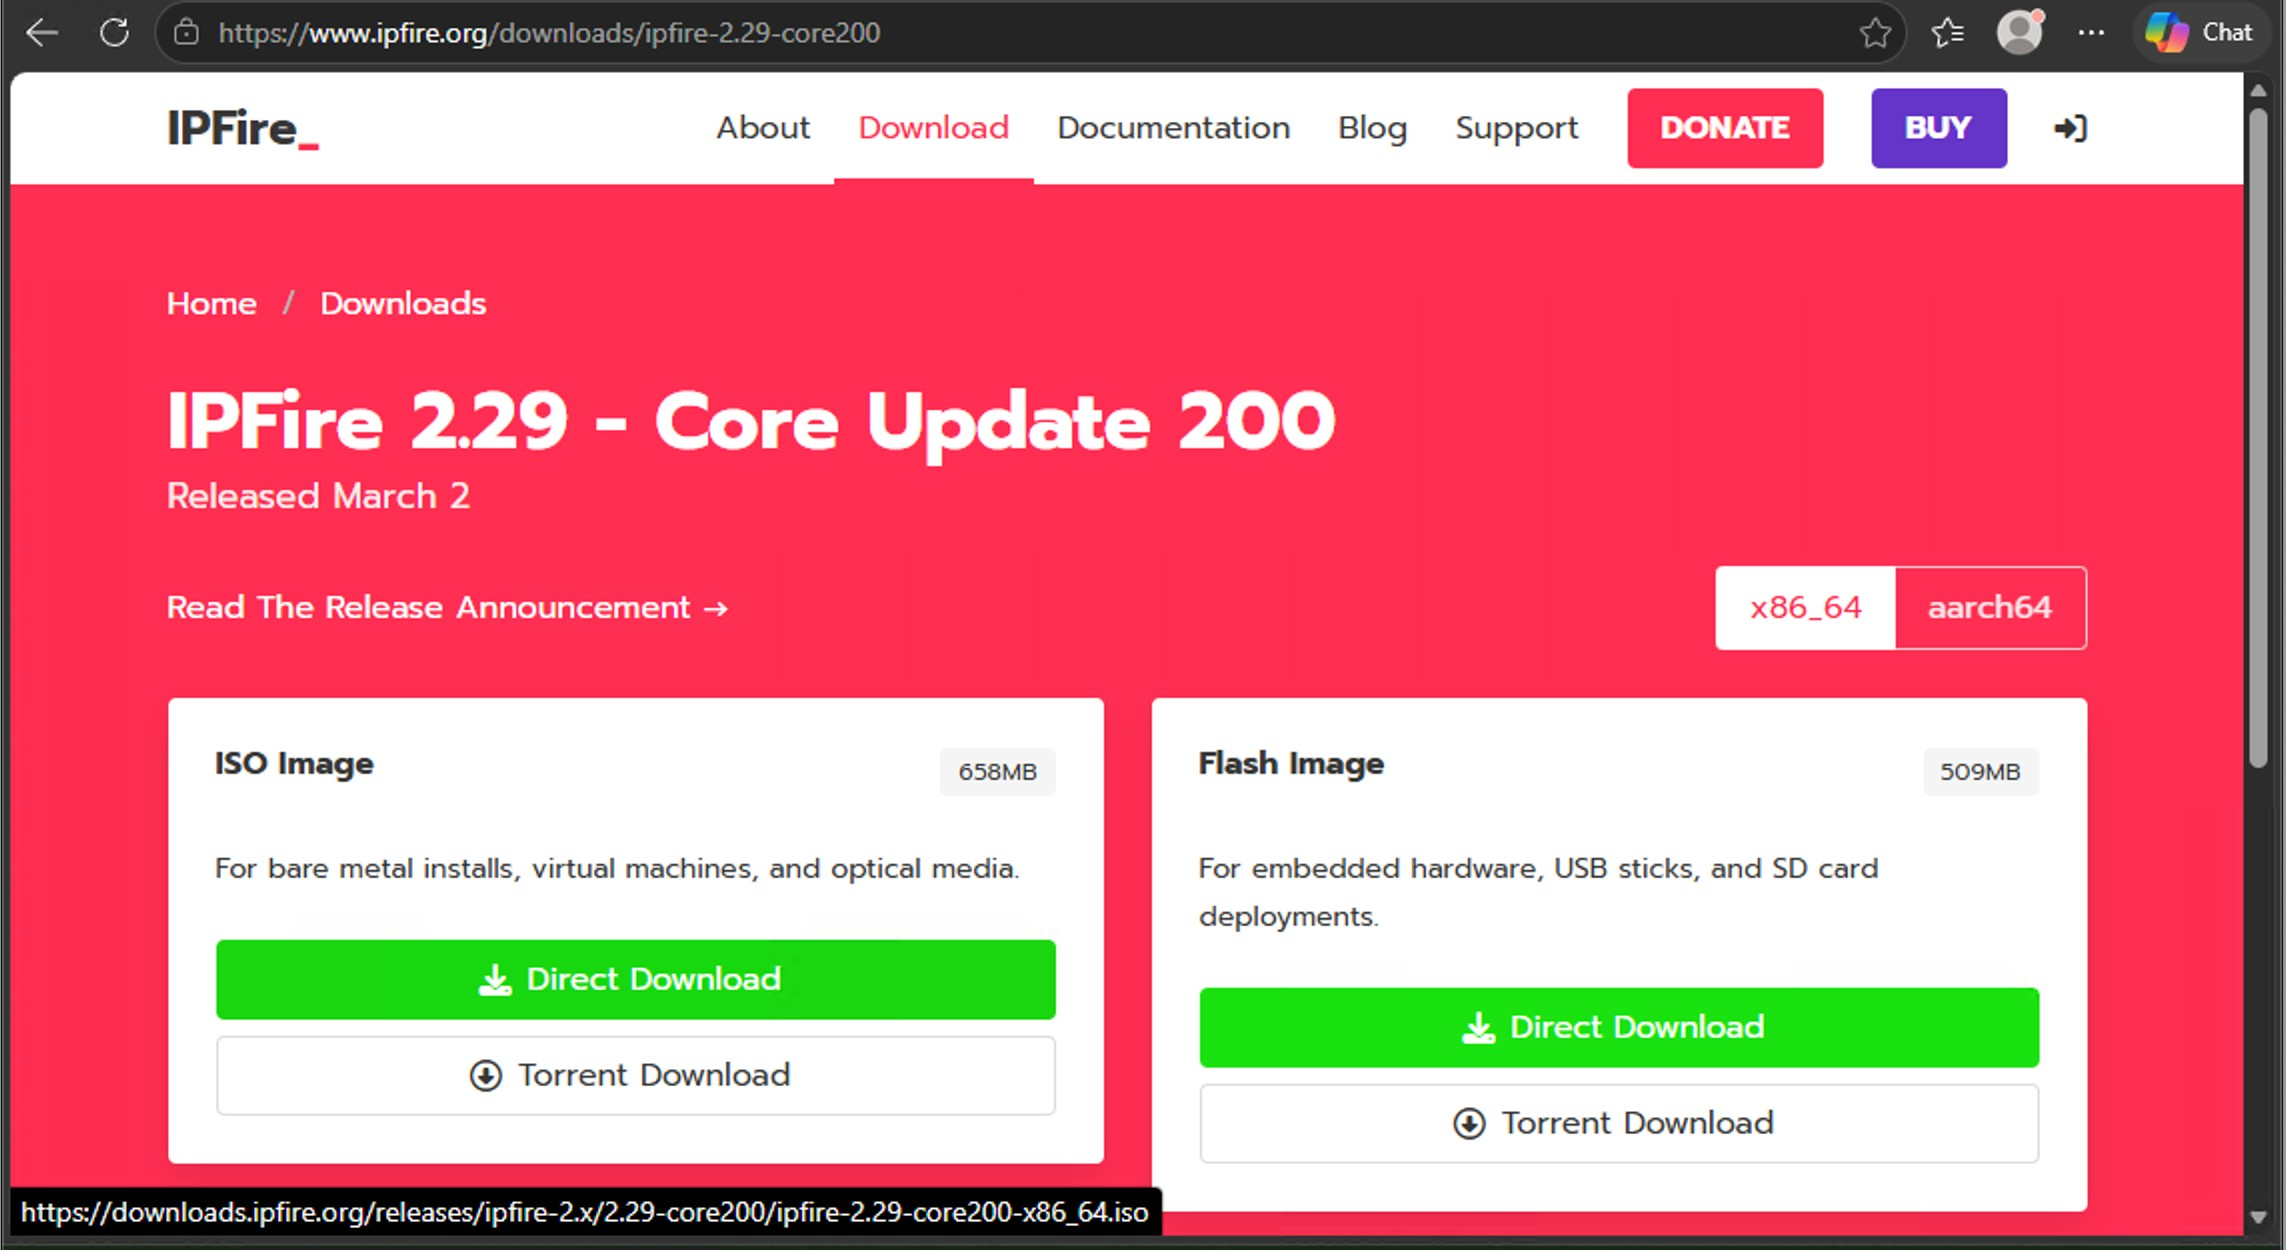
\includegraphics[width=0.9\textwidth]{media/ipfire/1.jpg}
	\caption{Pobieranie obrazu ISO}
	\label{fig:ipf_1}
\end{figure}

\subsection{Przygotowanie maszyny wirtualnej i instalacja systemu}
Przygotowujemy maszynę wirtualną do testowej konfiguracji w Oracle Virtualbox [Rys. \ref{fig:ipf_2}]. Podłączamy dwie karty sieciowe w trybie NAT i w trybie sieci wewnętrznej.
\begin{figure}[!htbp]
	\centering
	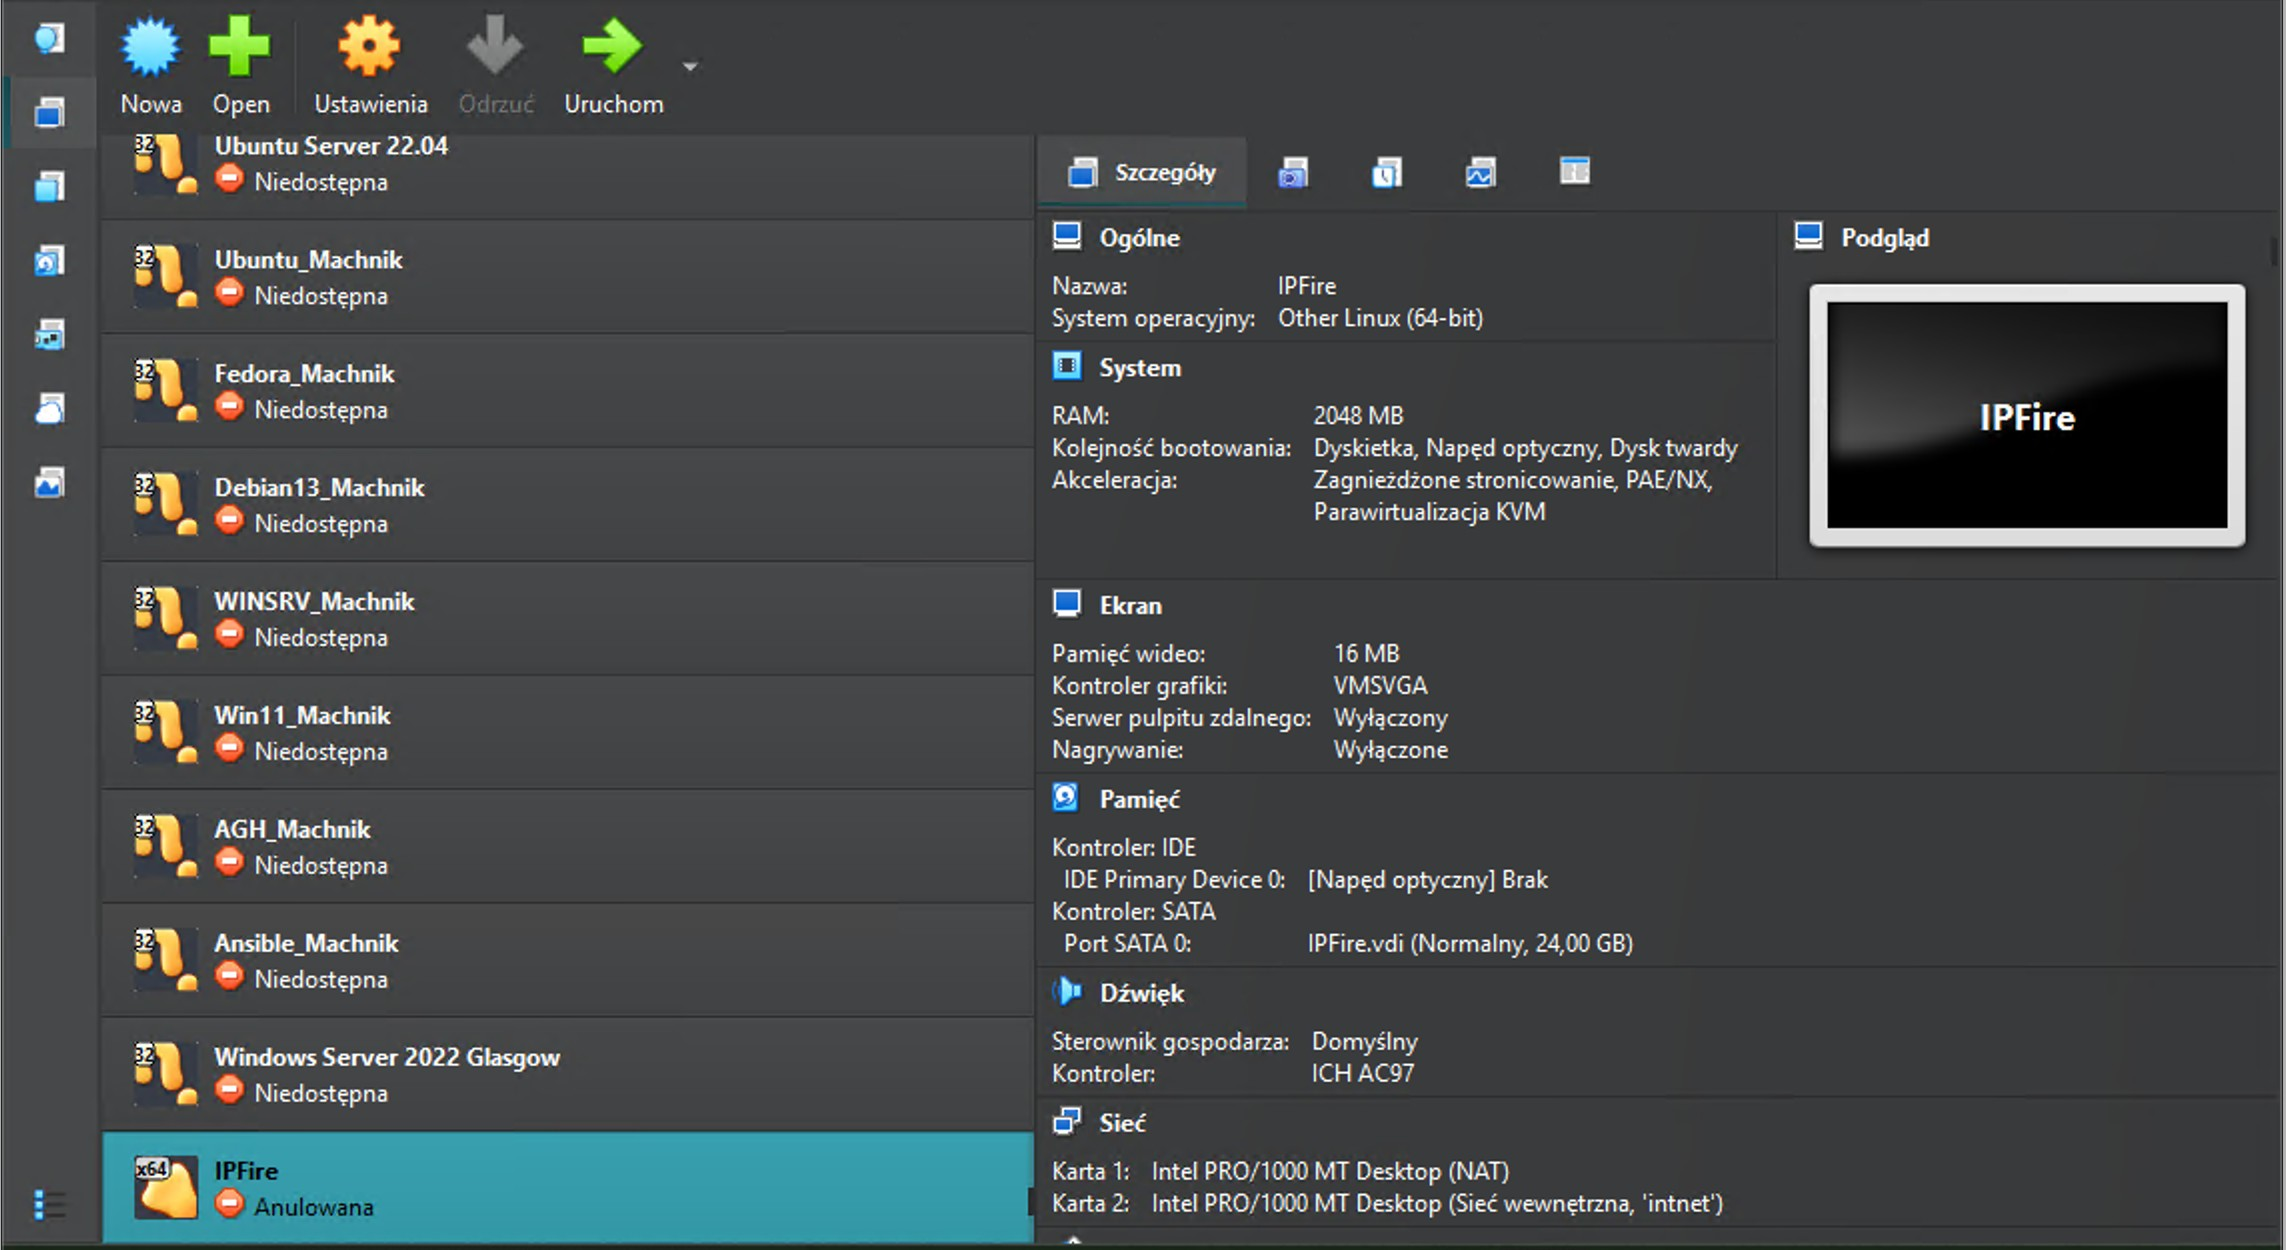
\includegraphics[width=0.9\textwidth]{media/ipfire/2.jpg}
	\caption{Utworzenie maszyny wirtualnej}
	\label{fig:ipf_2}
\end{figure}
Przy pierwszym uruchomieniu maszyny wirtualnej przechodzimy przez proces instalacyjny, który jest bardzo prosty, intuicyjny i nie odbiega wiele od instalacji innych dystrybucji Linuxa, takich jak np. Debian. Obejmuje między innymi wybór pakietu językowego, układu klawiatury, strefy czasowej, nazwy hosta, domeny, hasła użytkownika root i admina, za pomocą którego będziemy logować się do interfejsu webowego.

\subsection{Konfiguracja sieci}
Po zainstalowaniu systemu przechodzimy do jego wstępnej konfiguracji, gdzie kluczowa jest konfiguracja interfejsów sieciowych [Rys. \ref{fig:ipf_3}]
\begin{figure}[!htbp]
	\centering
	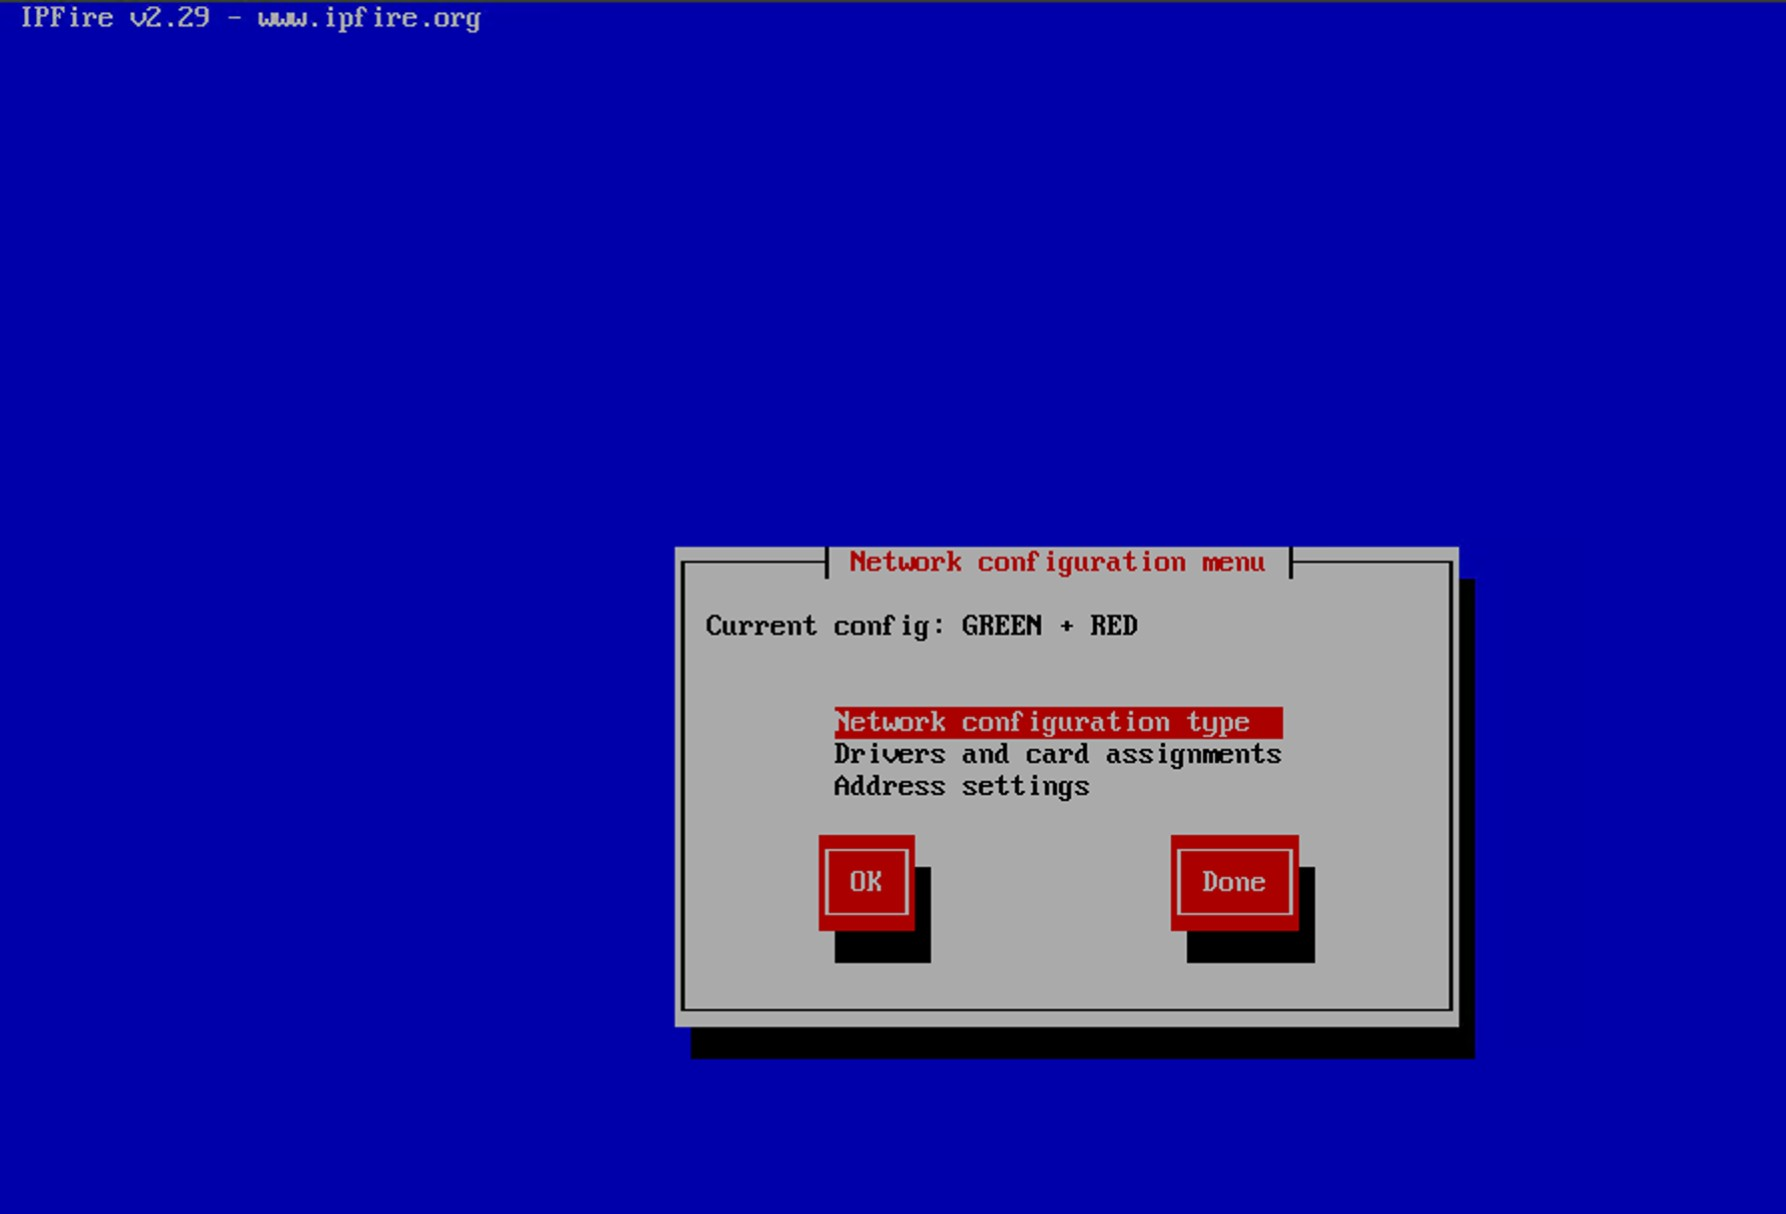
\includegraphics[width=0.9\textwidth]{media/ipfire/3.jpg}
	\caption{Menu konfiguracji sieci}
	\label{fig:ipf_3}
\end{figure}

\subsubsection{Network configuration type}
Wybieramy tutaj docelową architekturę podziału naszej sieci [Rys. \ref{fig:ipf_4}]
\begin{figure}[!htbp]
	\centering
	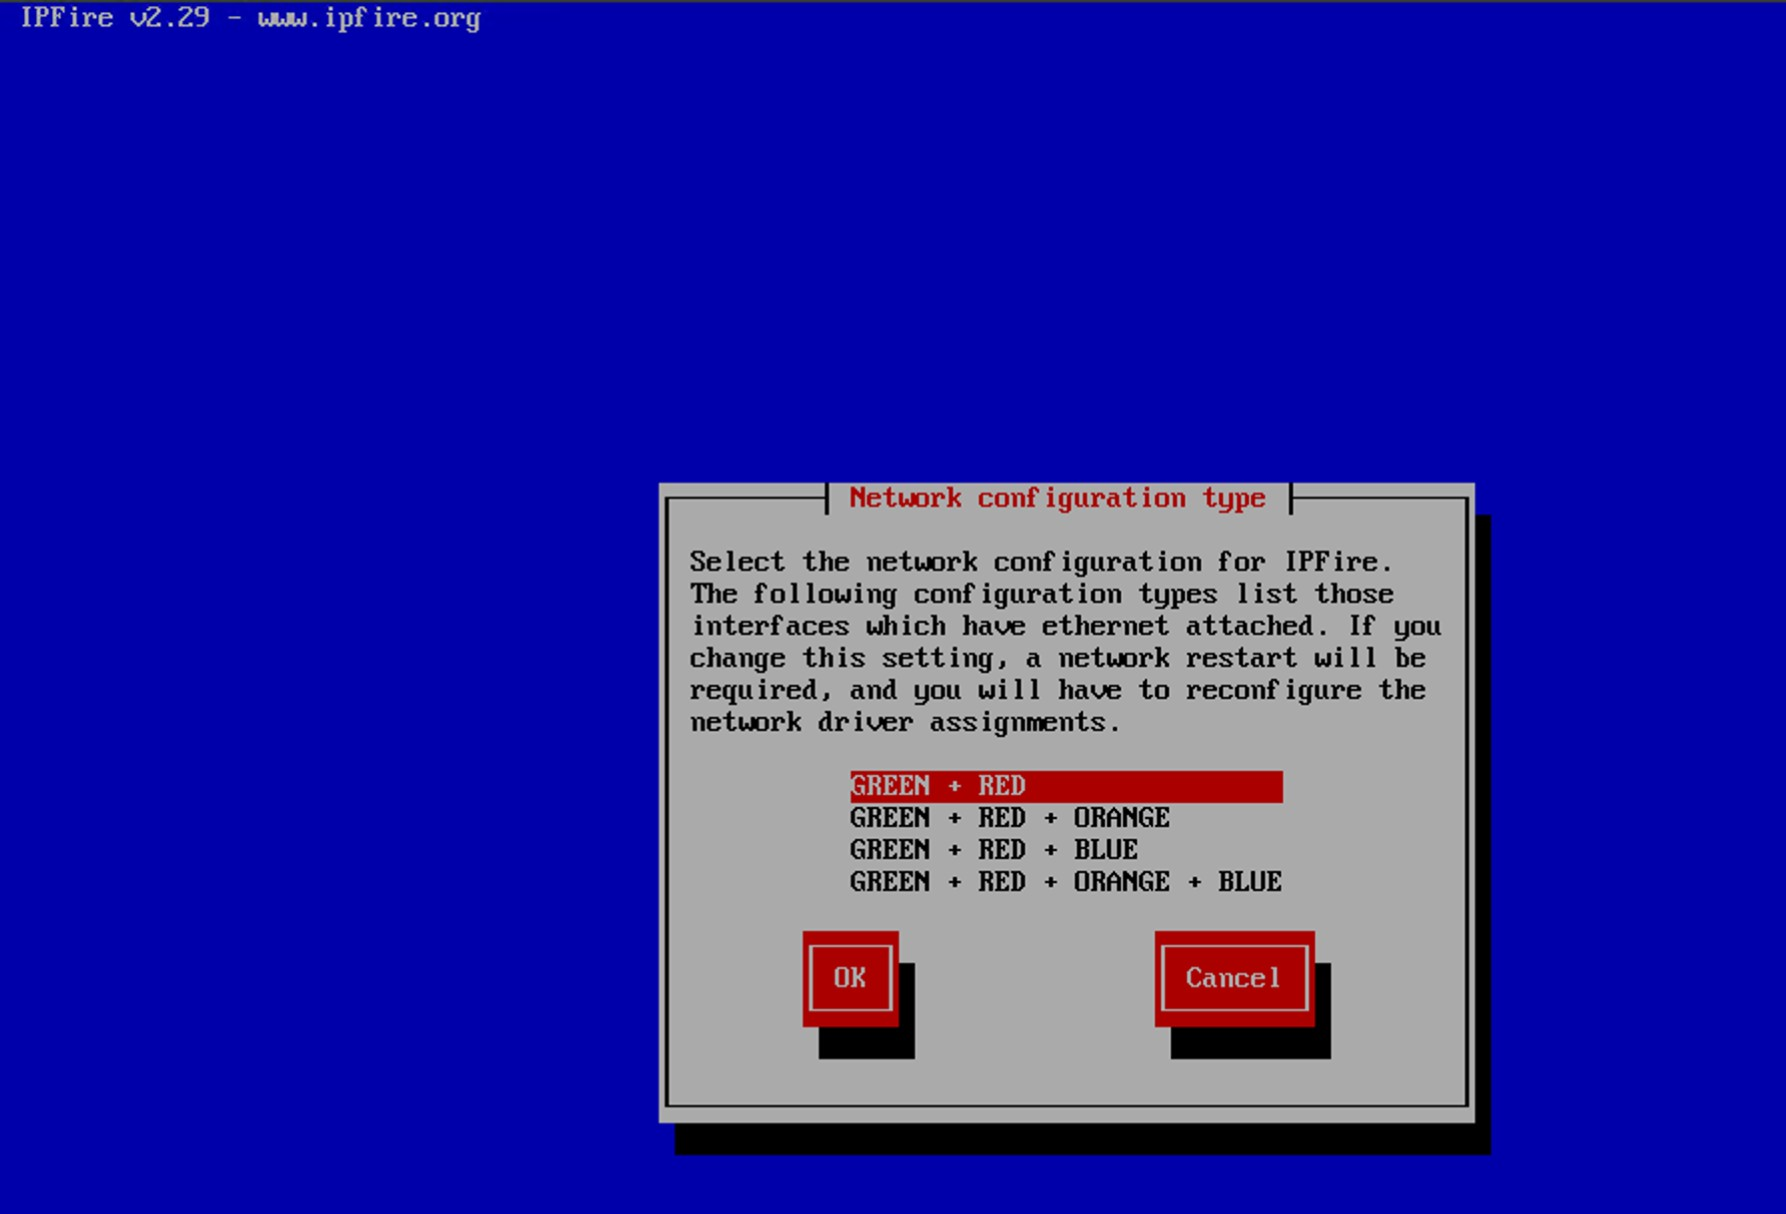
\includegraphics[width=0.9\textwidth]{media/ipfire/4.jpg}
	\caption{Wybór typów interfejsu}
	\label{fig:ipf_4}
\end{figure}

Domyślnie mamy wybrany najbardziej podstawowy podział, który sami zastosujemy w tej testowej konfiguracji: GREEN + RED, gdzie „GREEN” oznacza sieć lokalną, a „RED” oznacza sieć rozległą (np. Internet).

Pozostałe typy, które możemy objąć w naszej konfiguracji, to „BLUE” oznaczający sieć bezprzewodową (Wi-Fi) oraz „ORANGE” oznaczający sieć strefy zdemilitaryzowanej (DMZ).

\subsubsection{Drivers and card assignments}
Tutaj przypisujemy dostępne interfejsy sieciowe do poszczególnych typów (kolorów) wybranych w poprzednim kroku. [Rys. \ref{fig:ipf_5}]
\begin{figure}[!htbp]
	\centering
	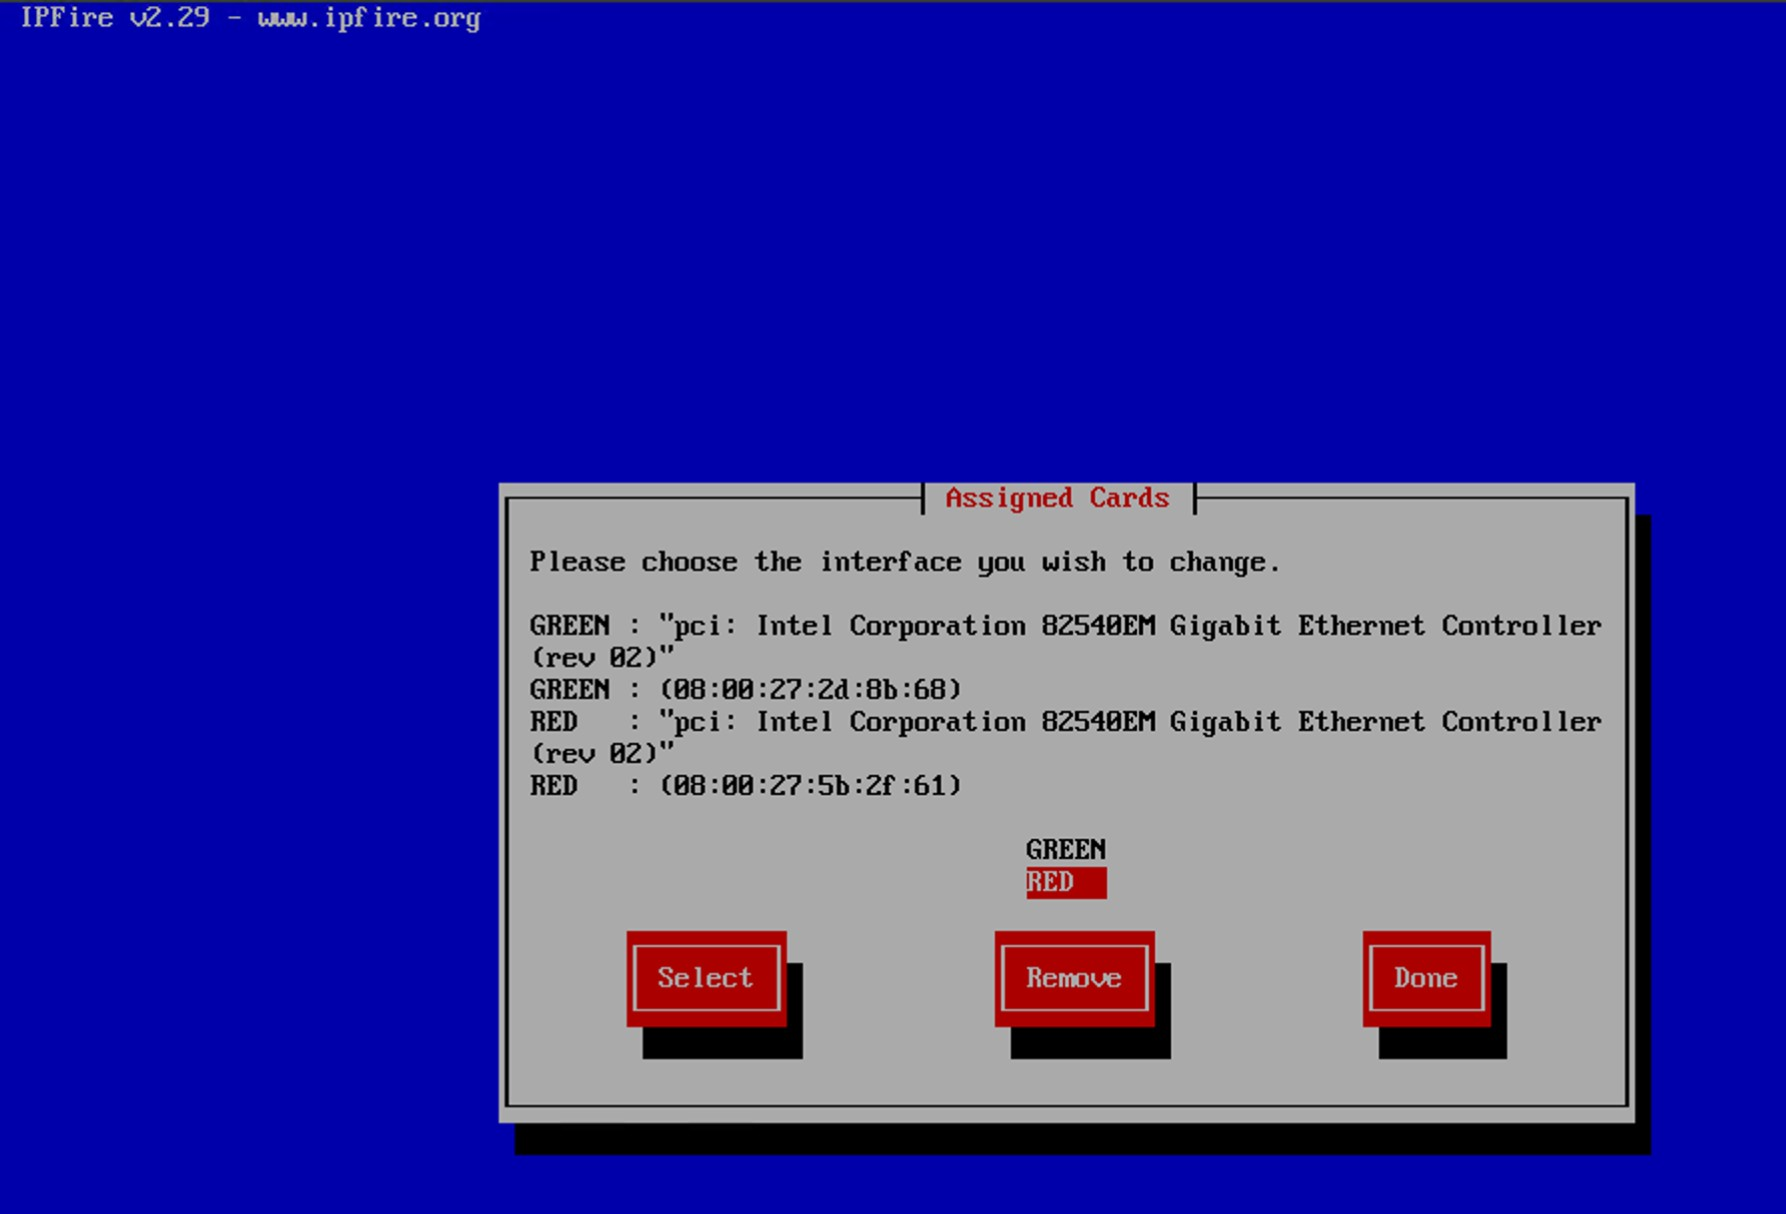
\includegraphics[width=0.9\textwidth]{media/ipfire/5.jpg}
	\caption{Przypisanie dostępnych interfejsów do wybranych stref}
	\label{fig:ipf_5}
\end{figure}

\subsubsection{Address settings}
Wreszcie dokonujemy konfiguracji adresacji IP wybranych interfejsów. Sieci lokalnej „GREEN” przypisujemy adresację 10.0.0.0/24 [Rys. \ref{fig:ipf_6}], natomiast interfejs „RED” konfigurujemy z wykorzystaniem protokołu DHCP. [Rys. \ref{fig:ipf_7}]
\begin{figure}[!htbp]
	\centering
	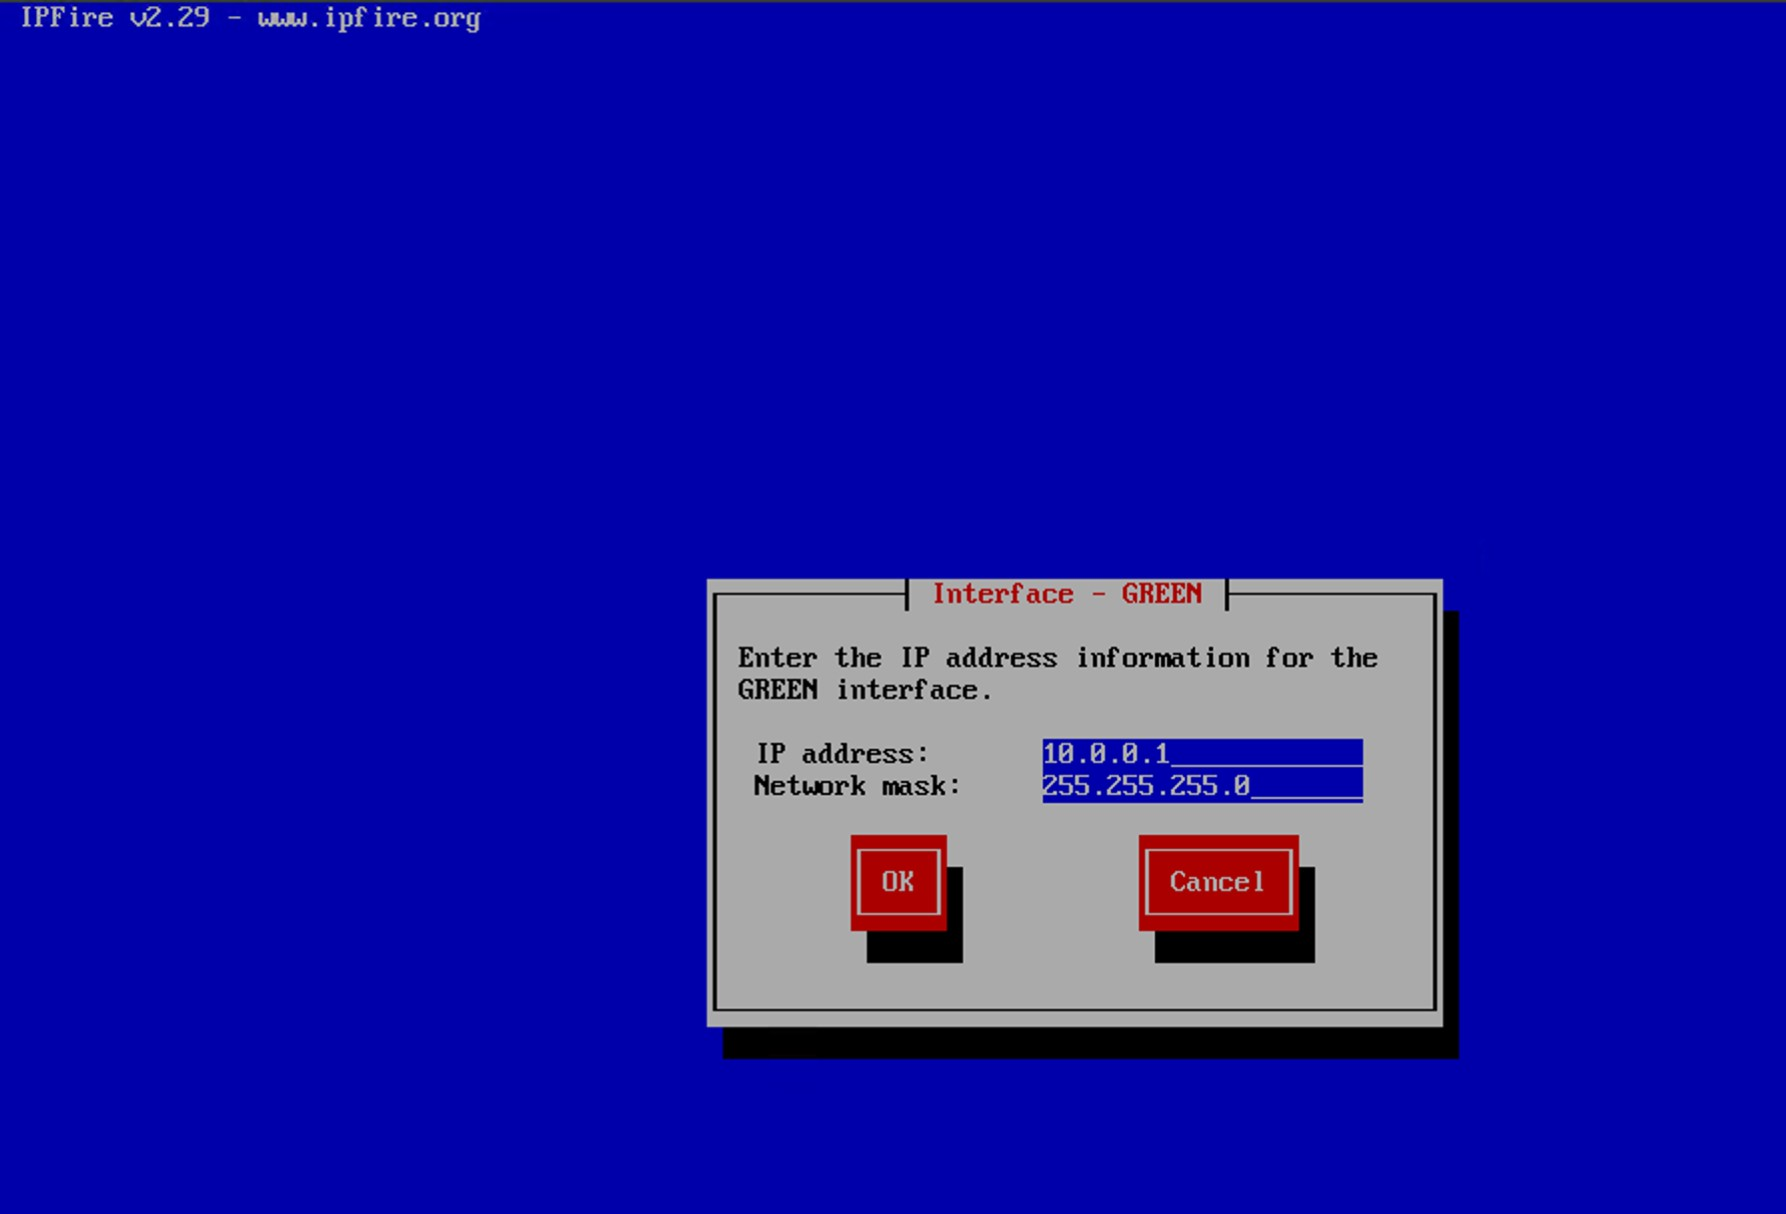
\includegraphics[width=0.9\textwidth]{media/ipfire/6.jpg}
	\caption{Konfiguracja adresacji interfejsu GREEN}
	\label{fig:ipf_6}
\end{figure}
\begin{figure}[!htbp]
	\centering
	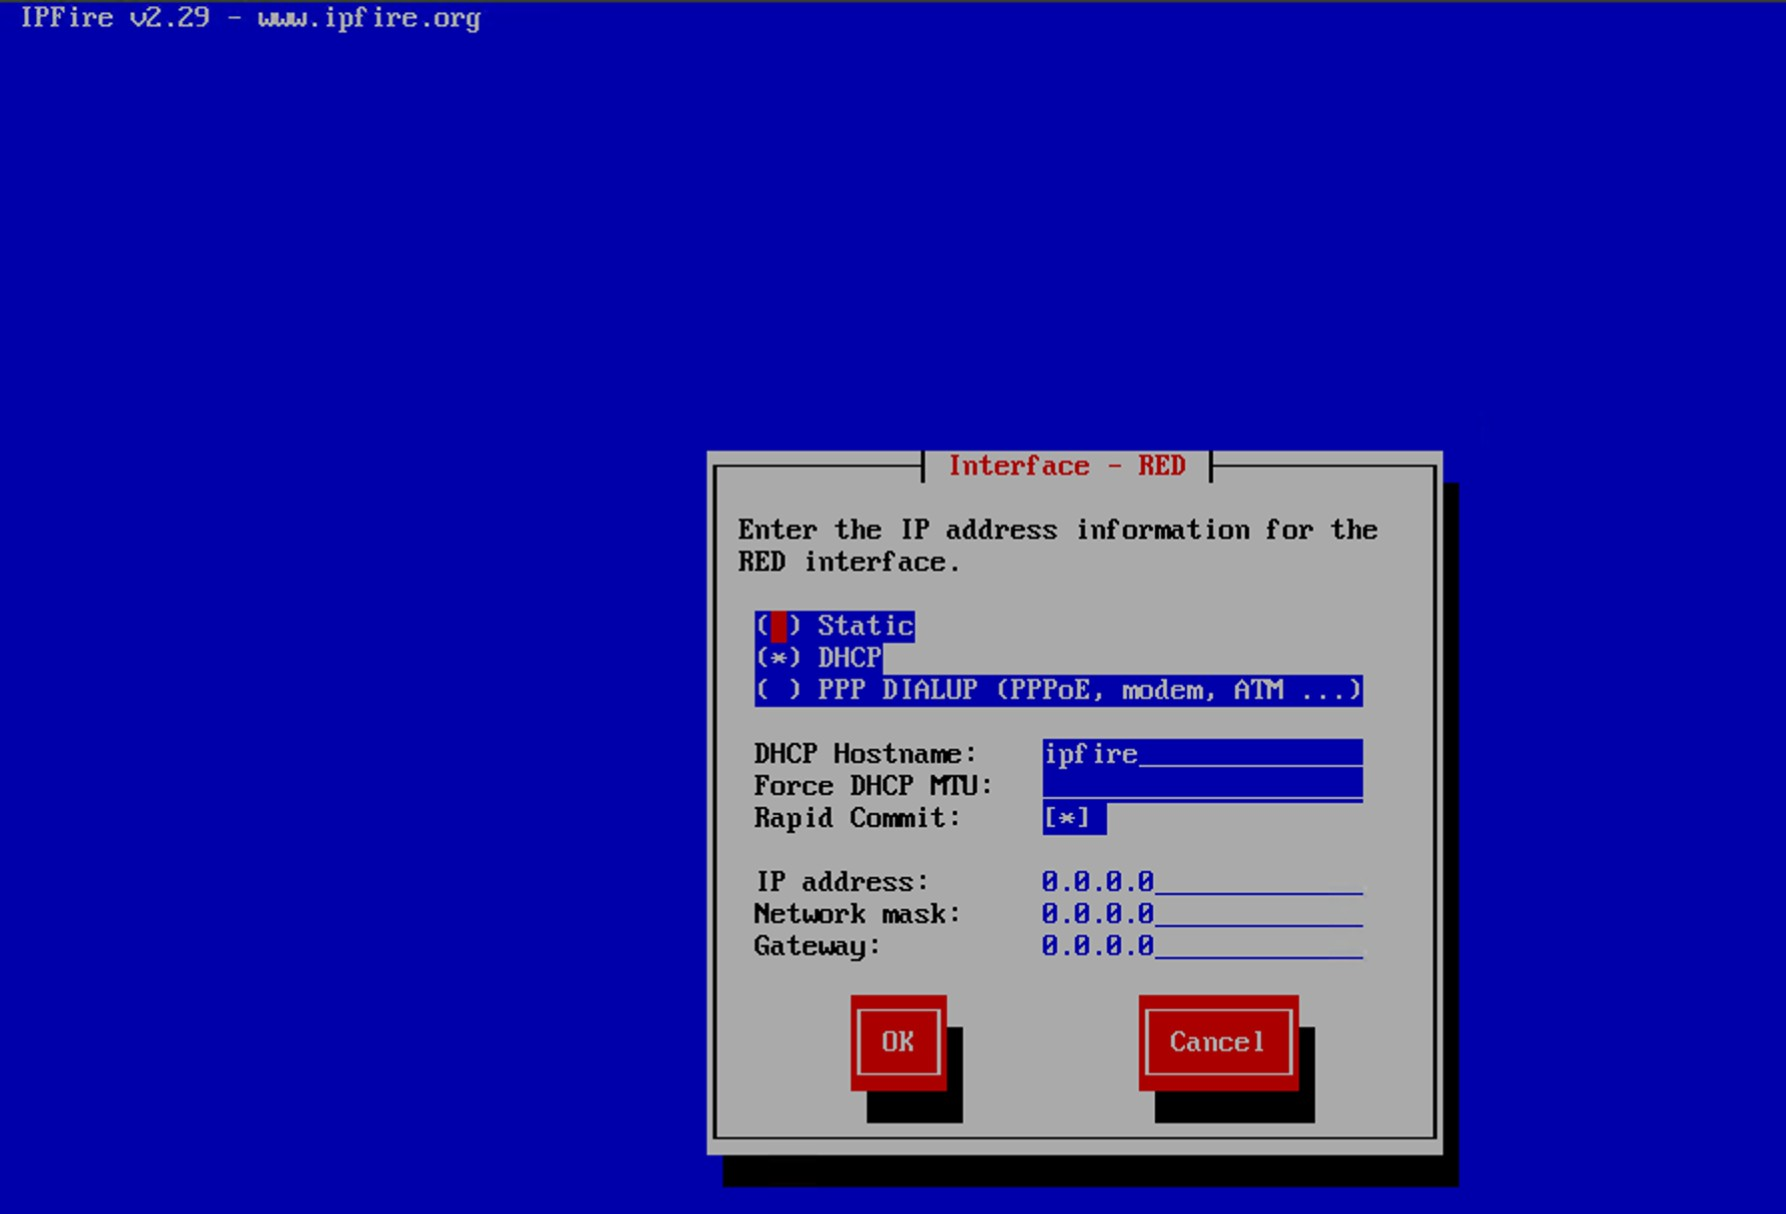
\includegraphics[width=0.9\textwidth]{media/ipfire/7.jpg}
	\caption{Konfiguracja adresacji interfejsu RED}
	\label{fig:ipf_7}
\end{figure}

\subsection{Konfiguracja serwera DHCP}
W następnym kroku możemy przeprowadzić konfigurację serwera DHCP dla sieci lokalnej [Rys. \ref{fig:ipf_8}]
\begin{figure}[!htbp]
	\centering
	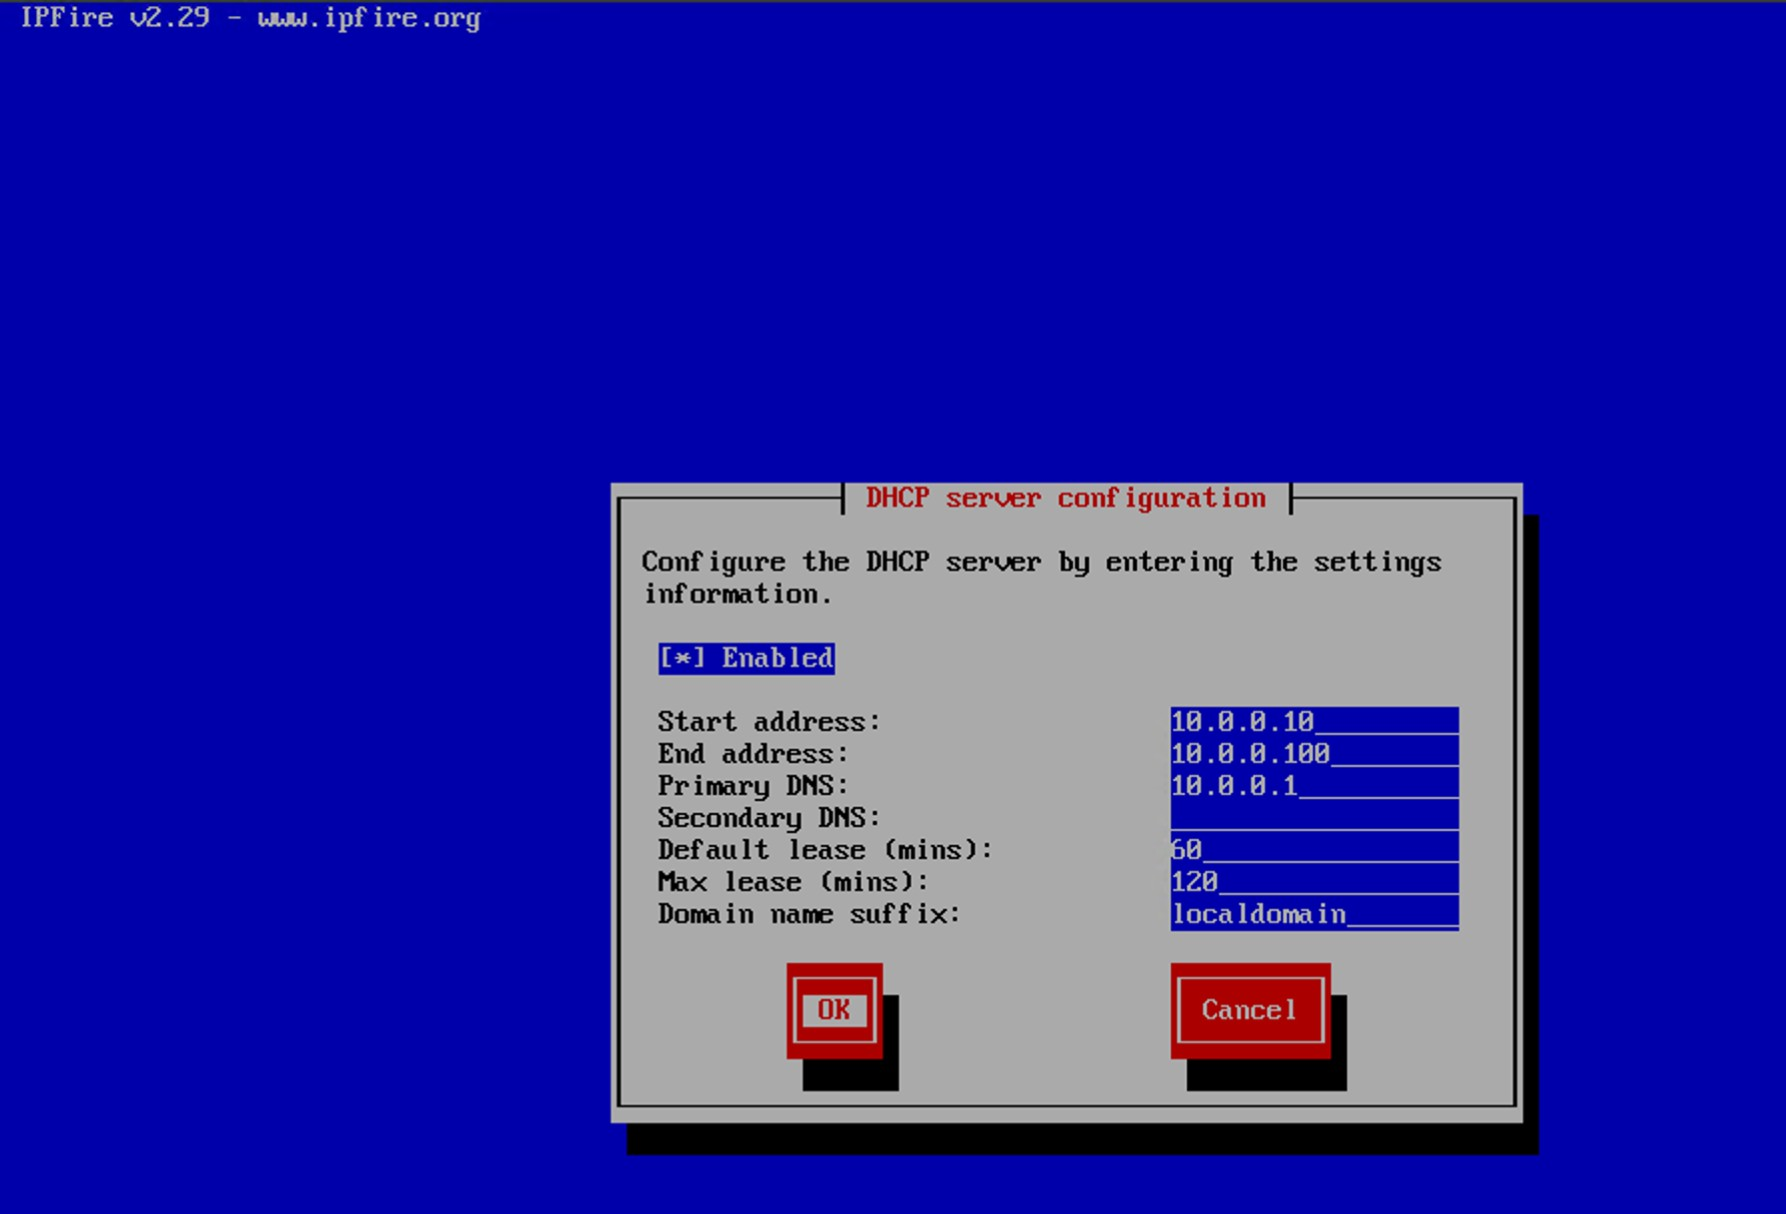
\includegraphics[width=0.9\textwidth]{media/ipfire/8.jpg}
	\caption{Konfiguracja serwera DHCP dla interfejsu GREEN}
	\label{fig:ipf_8}
\end{figure}

\subsection{Zakończenie instalacji}
System z powodzeniem dokończył konfigurację [Rys. \ref{fig:ipf_9}], uzyskał dane adresowe na interfejsie „RED” [Rys. \ref{fig:ipf_10}]. Możemy zalogować się przez CLI lub przez GUI.

Po uruchomieniu maszyny klienta od razu mamy dostęp do Internetu. Została pobrana prawidłowa konfiguracja przez DHCP. [Rys. \ref{fig:ipf_11}]

\begin{figure}[!htbp]
	\centering
	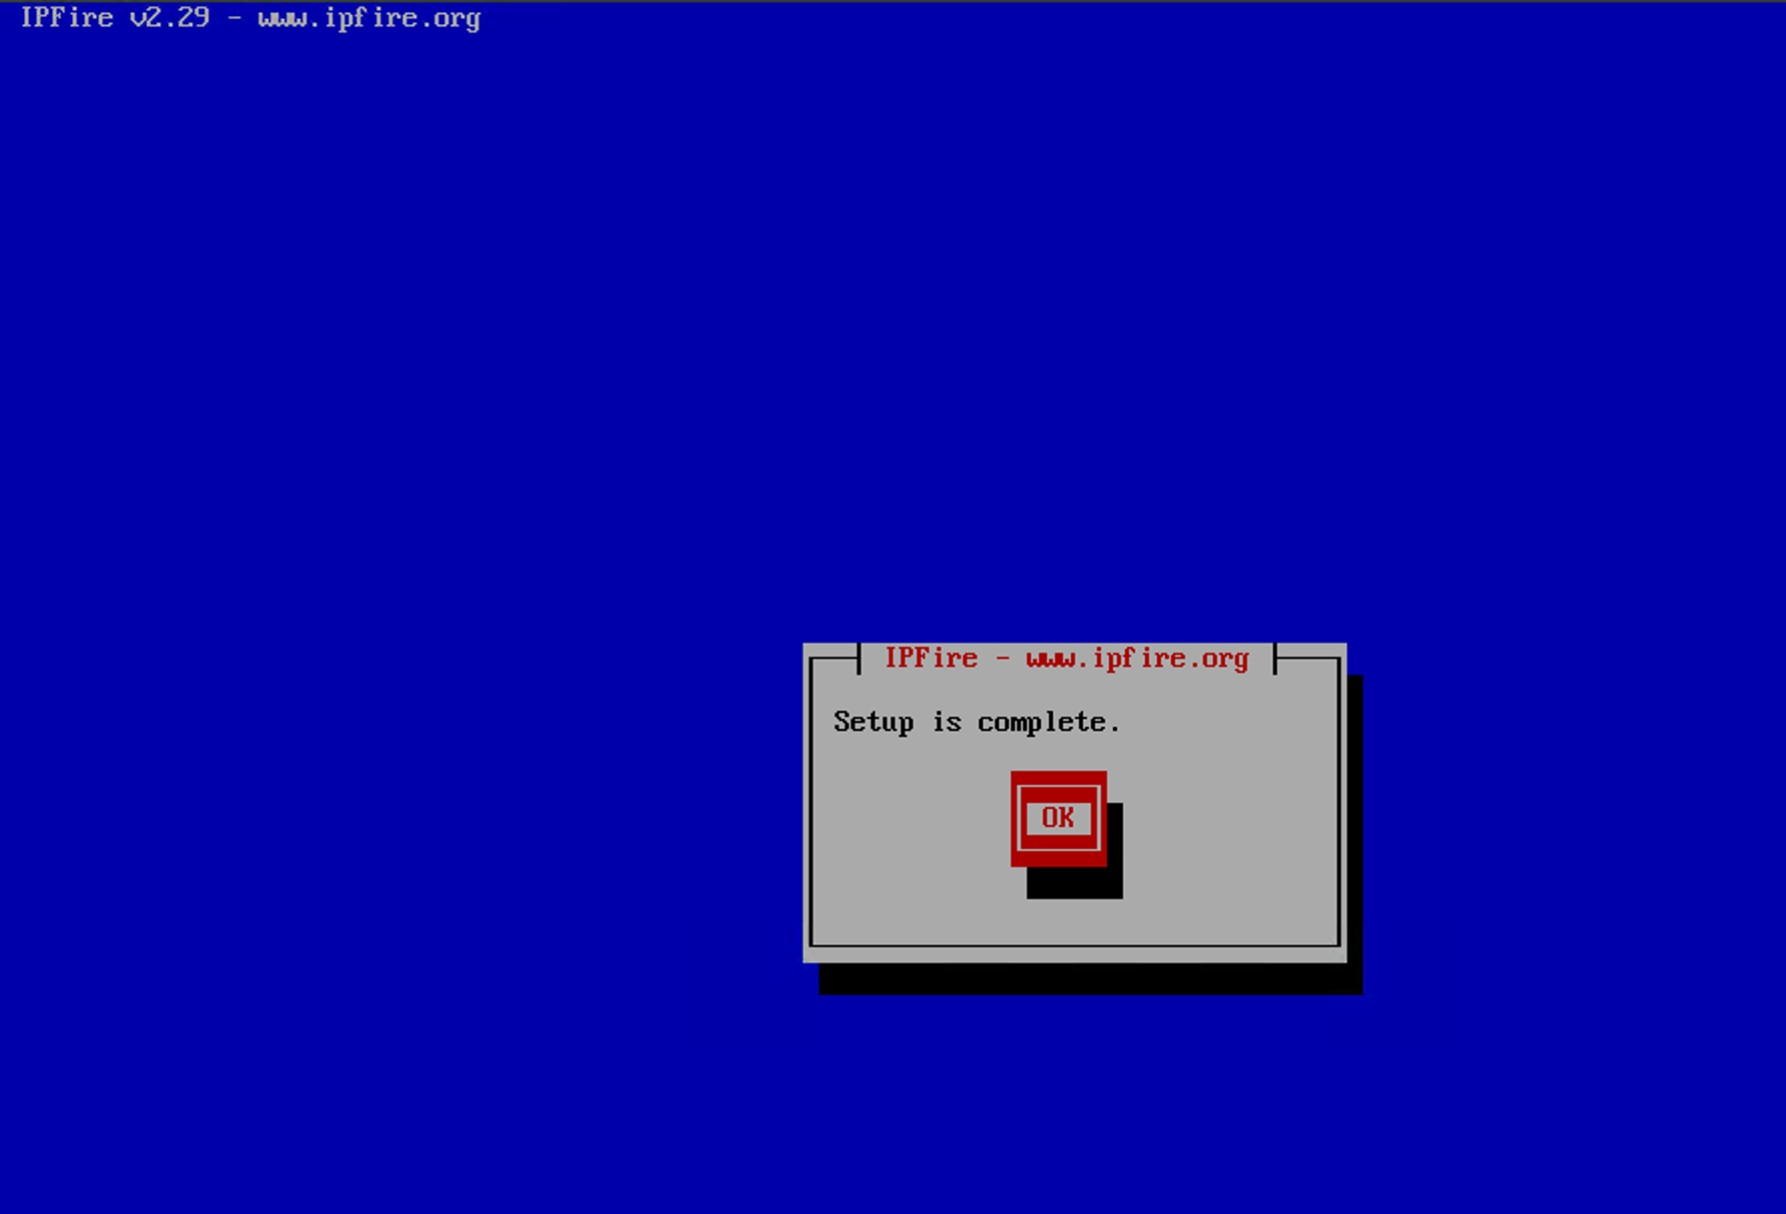
\includegraphics[width=0.9\textwidth]{media/ipfire/9.jpg}
	\caption{Zakończenie wstępnej konfiguracji poinstalacyjnej}
	\label{fig:ipf_9}
\end{figure}
\begin{figure}[!htbp]
	\centering
	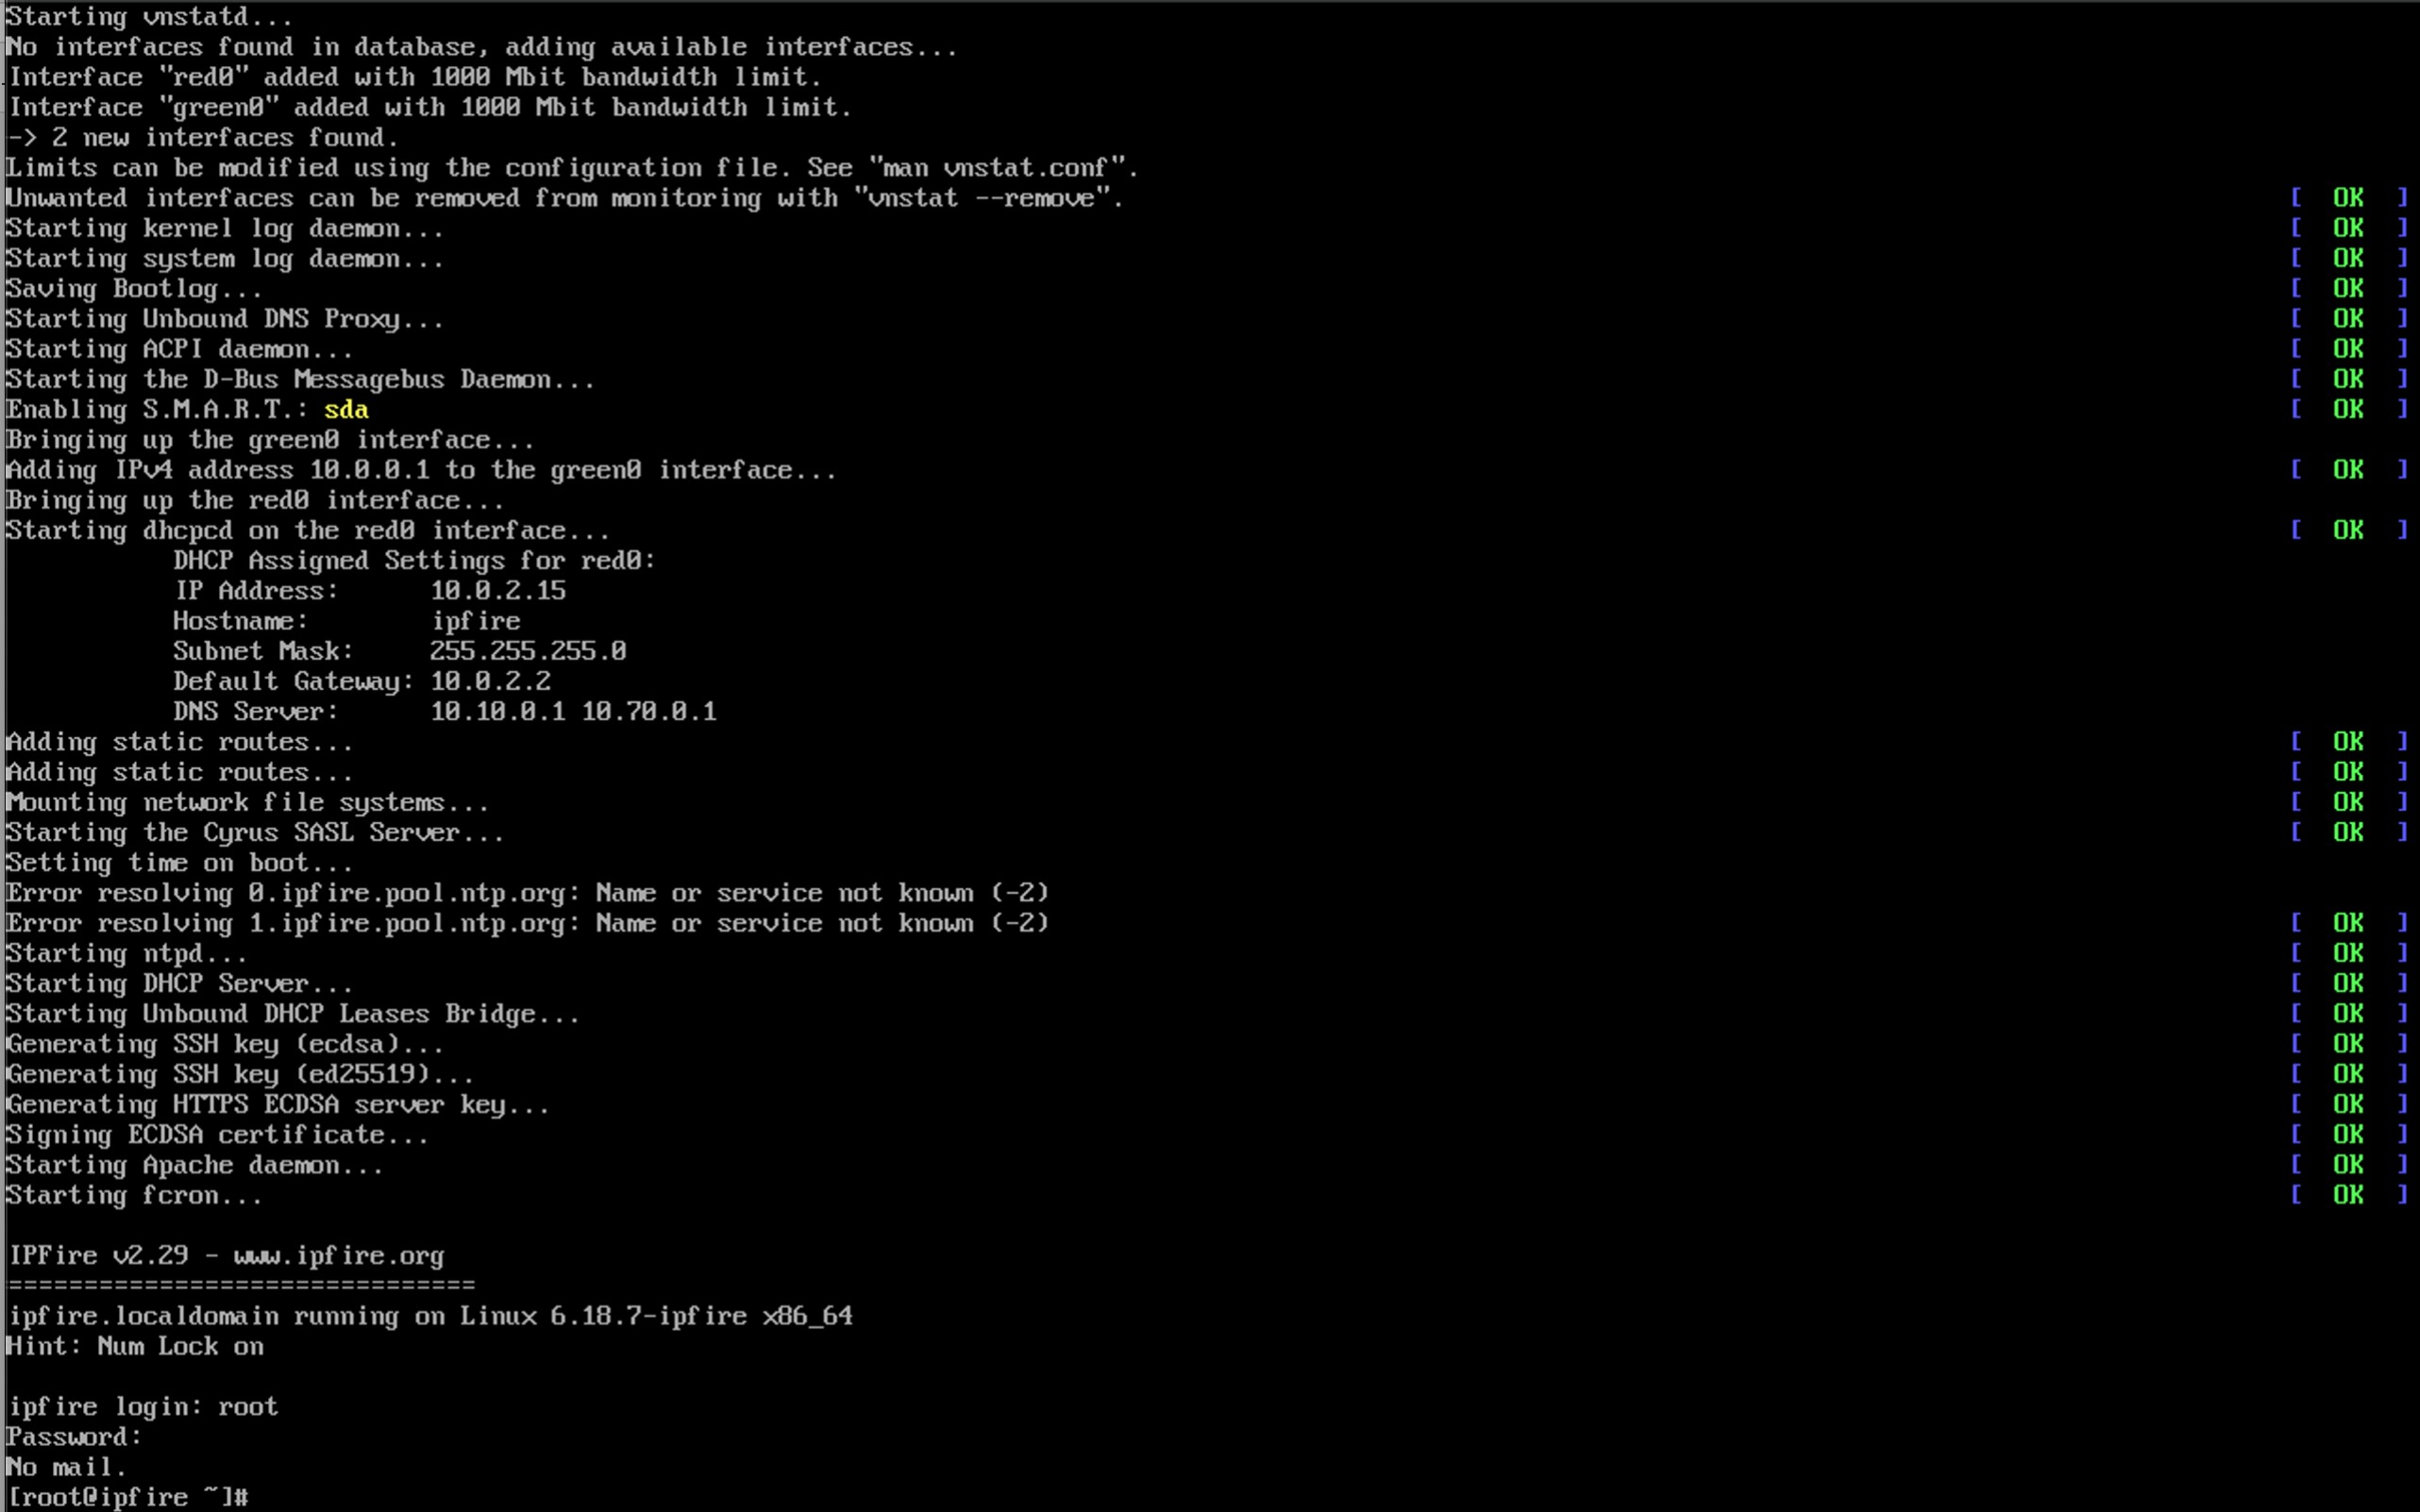
\includegraphics[width=0.9\textwidth]{media/ipfire/10.jpg}
	\caption{Pierwsze uzyskanie dostępu do systemu przez CLI}
	\label{fig:ipf_10}
\end{figure}
\begin{figure}[!htbp]
	\centering
	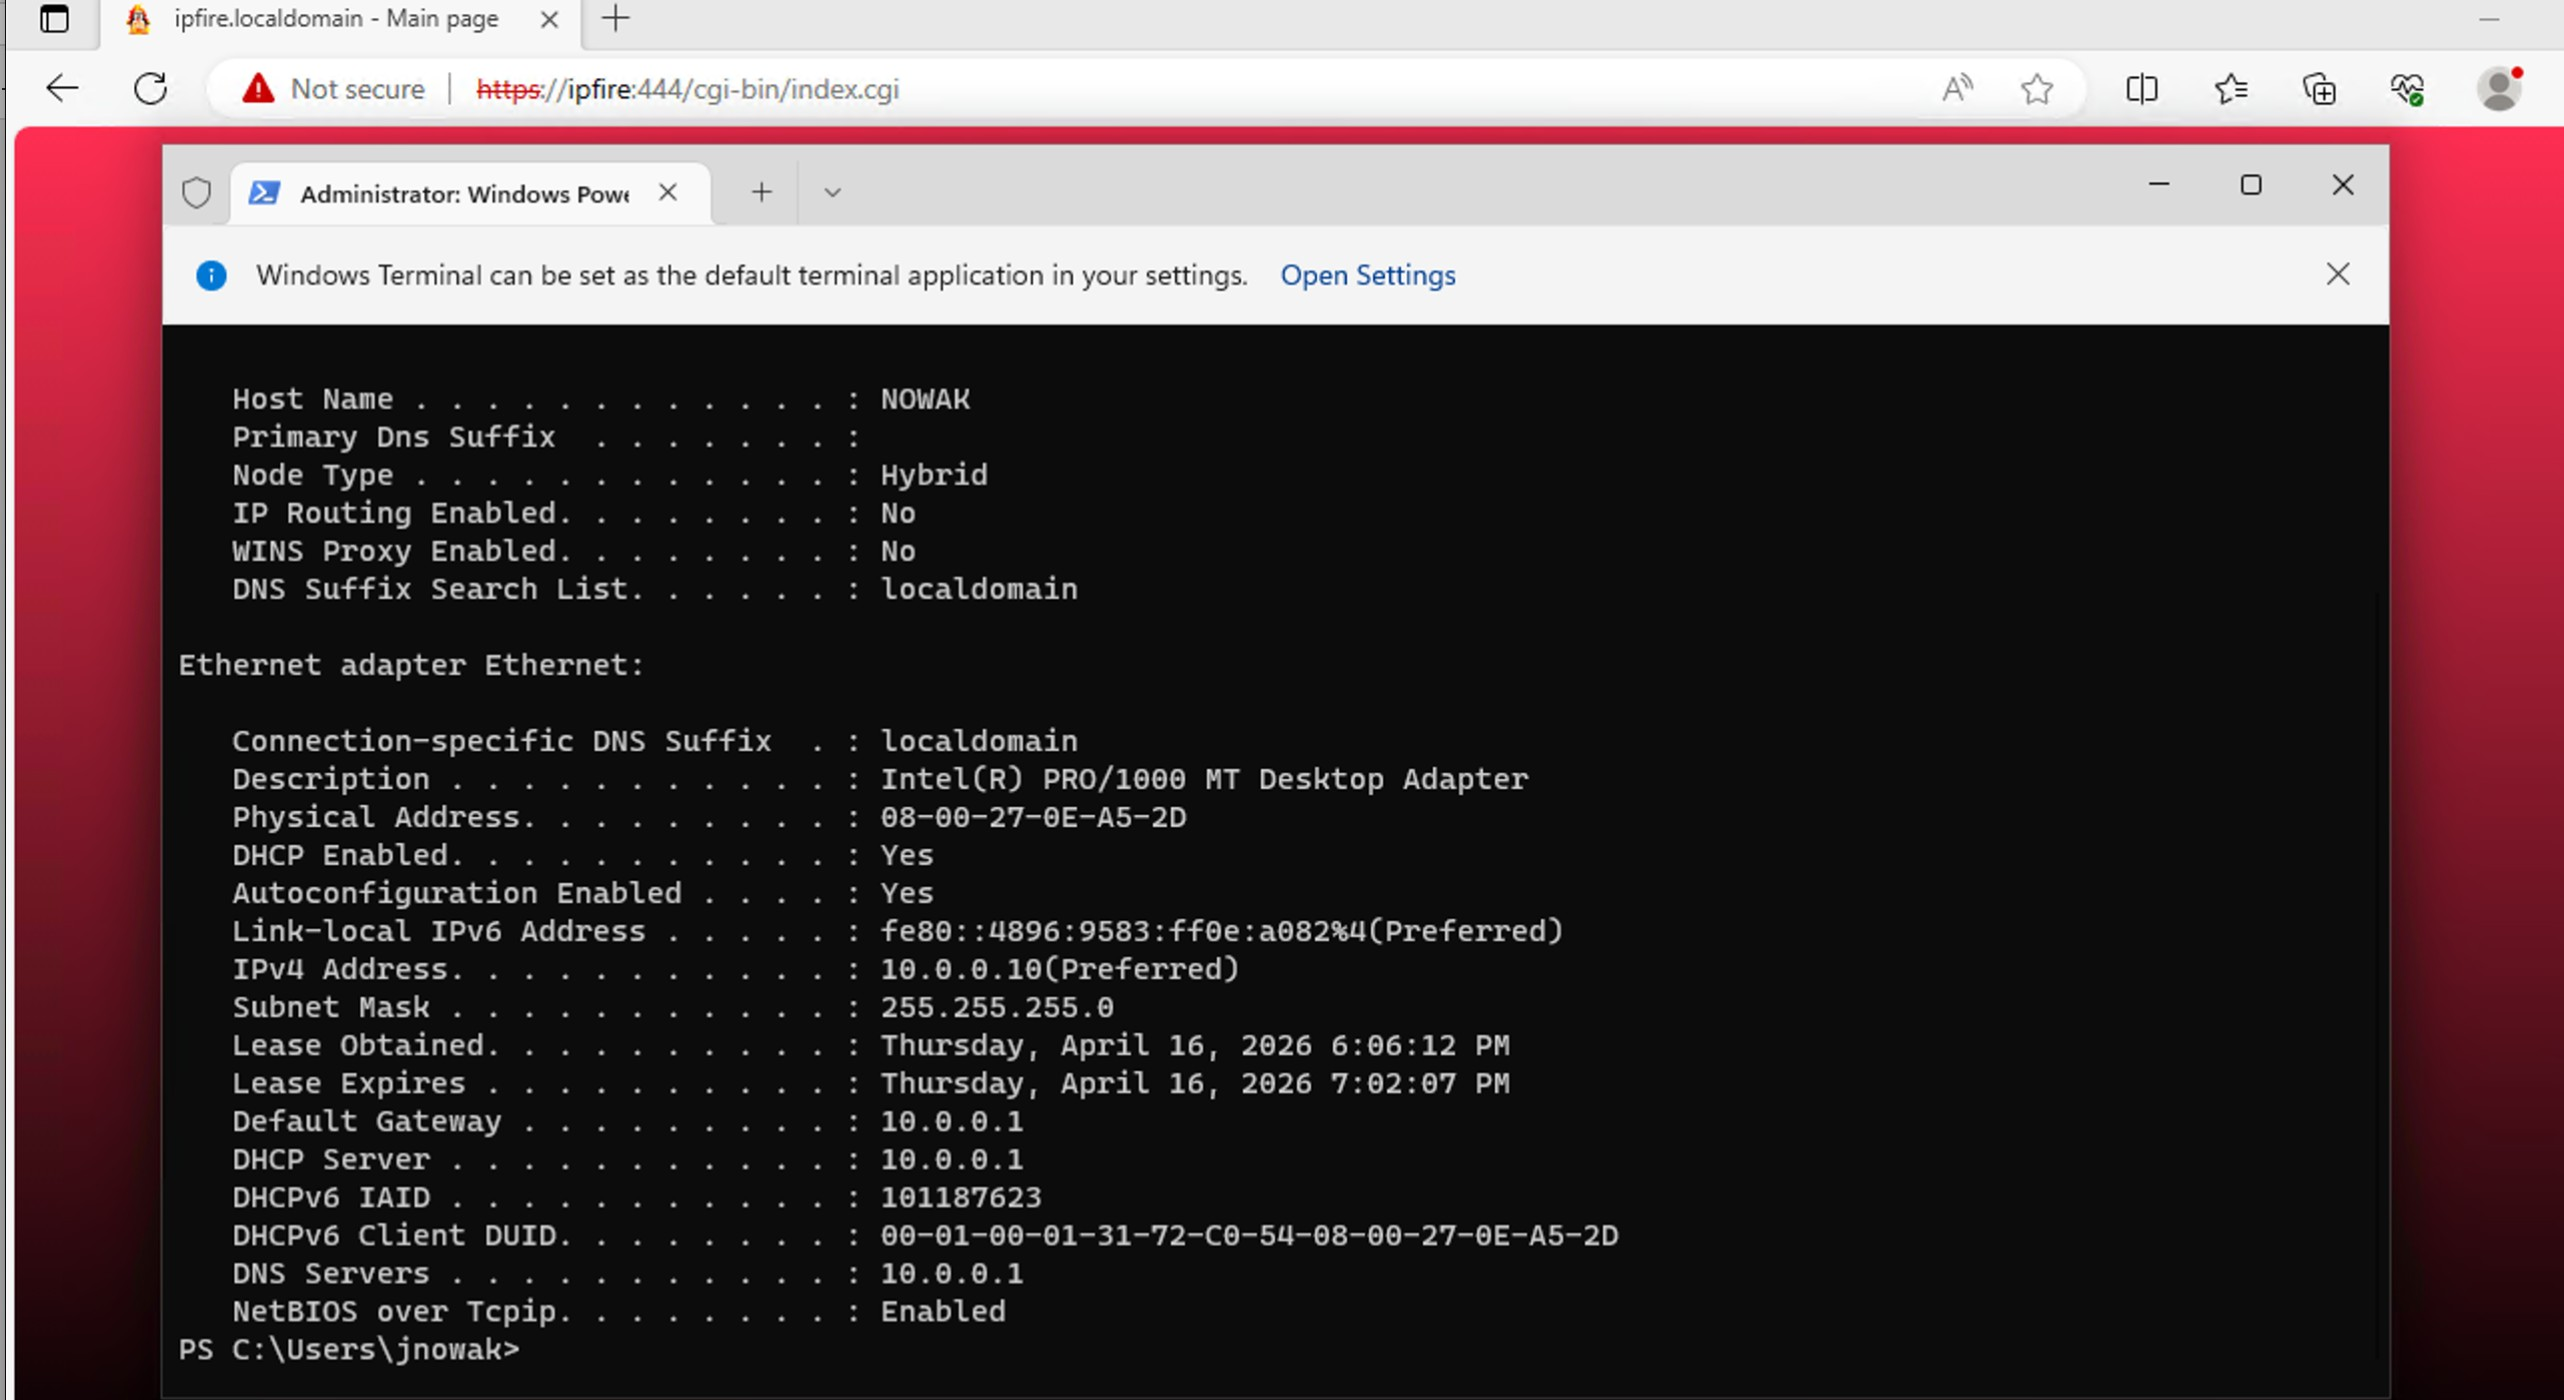
\includegraphics[width=0.9\textwidth]{media/ipfire/11.jpg}
	\caption{Uzyskana konfiguracja IP z serwera DHCP}
	\label{fig:ipf_11}
\end{figure}

\subsection{Interfejs zarządzania}
Aby uzyskać dostęp do konsoli wpisujemy w pasku przeglądarki https://ipfire:444, gdzie ipfire to nazwa hosta skonfigurowana przy instalacji systemu. Po uruchomieniu strony logujemy się na konto admina, którego hasło również konfigurowaliśmy w trakcie instalacji systemu.
\subsubsection{Zakładka System}
Podstawowe ustawienia i ogólne informacje o systemie operacyjnym. Można tu m.in. zarządzać powiadomieniami wysyłanymi przez Email, dostępem SSH, kopiami zapasowymi, zobaczyć informacje o stanie poszczególnych interfejsów, podatności sprzętowych itp. [Rys. \ref{fig:ipf_12}]
\begin{figure}[!htbp]
	\centering
	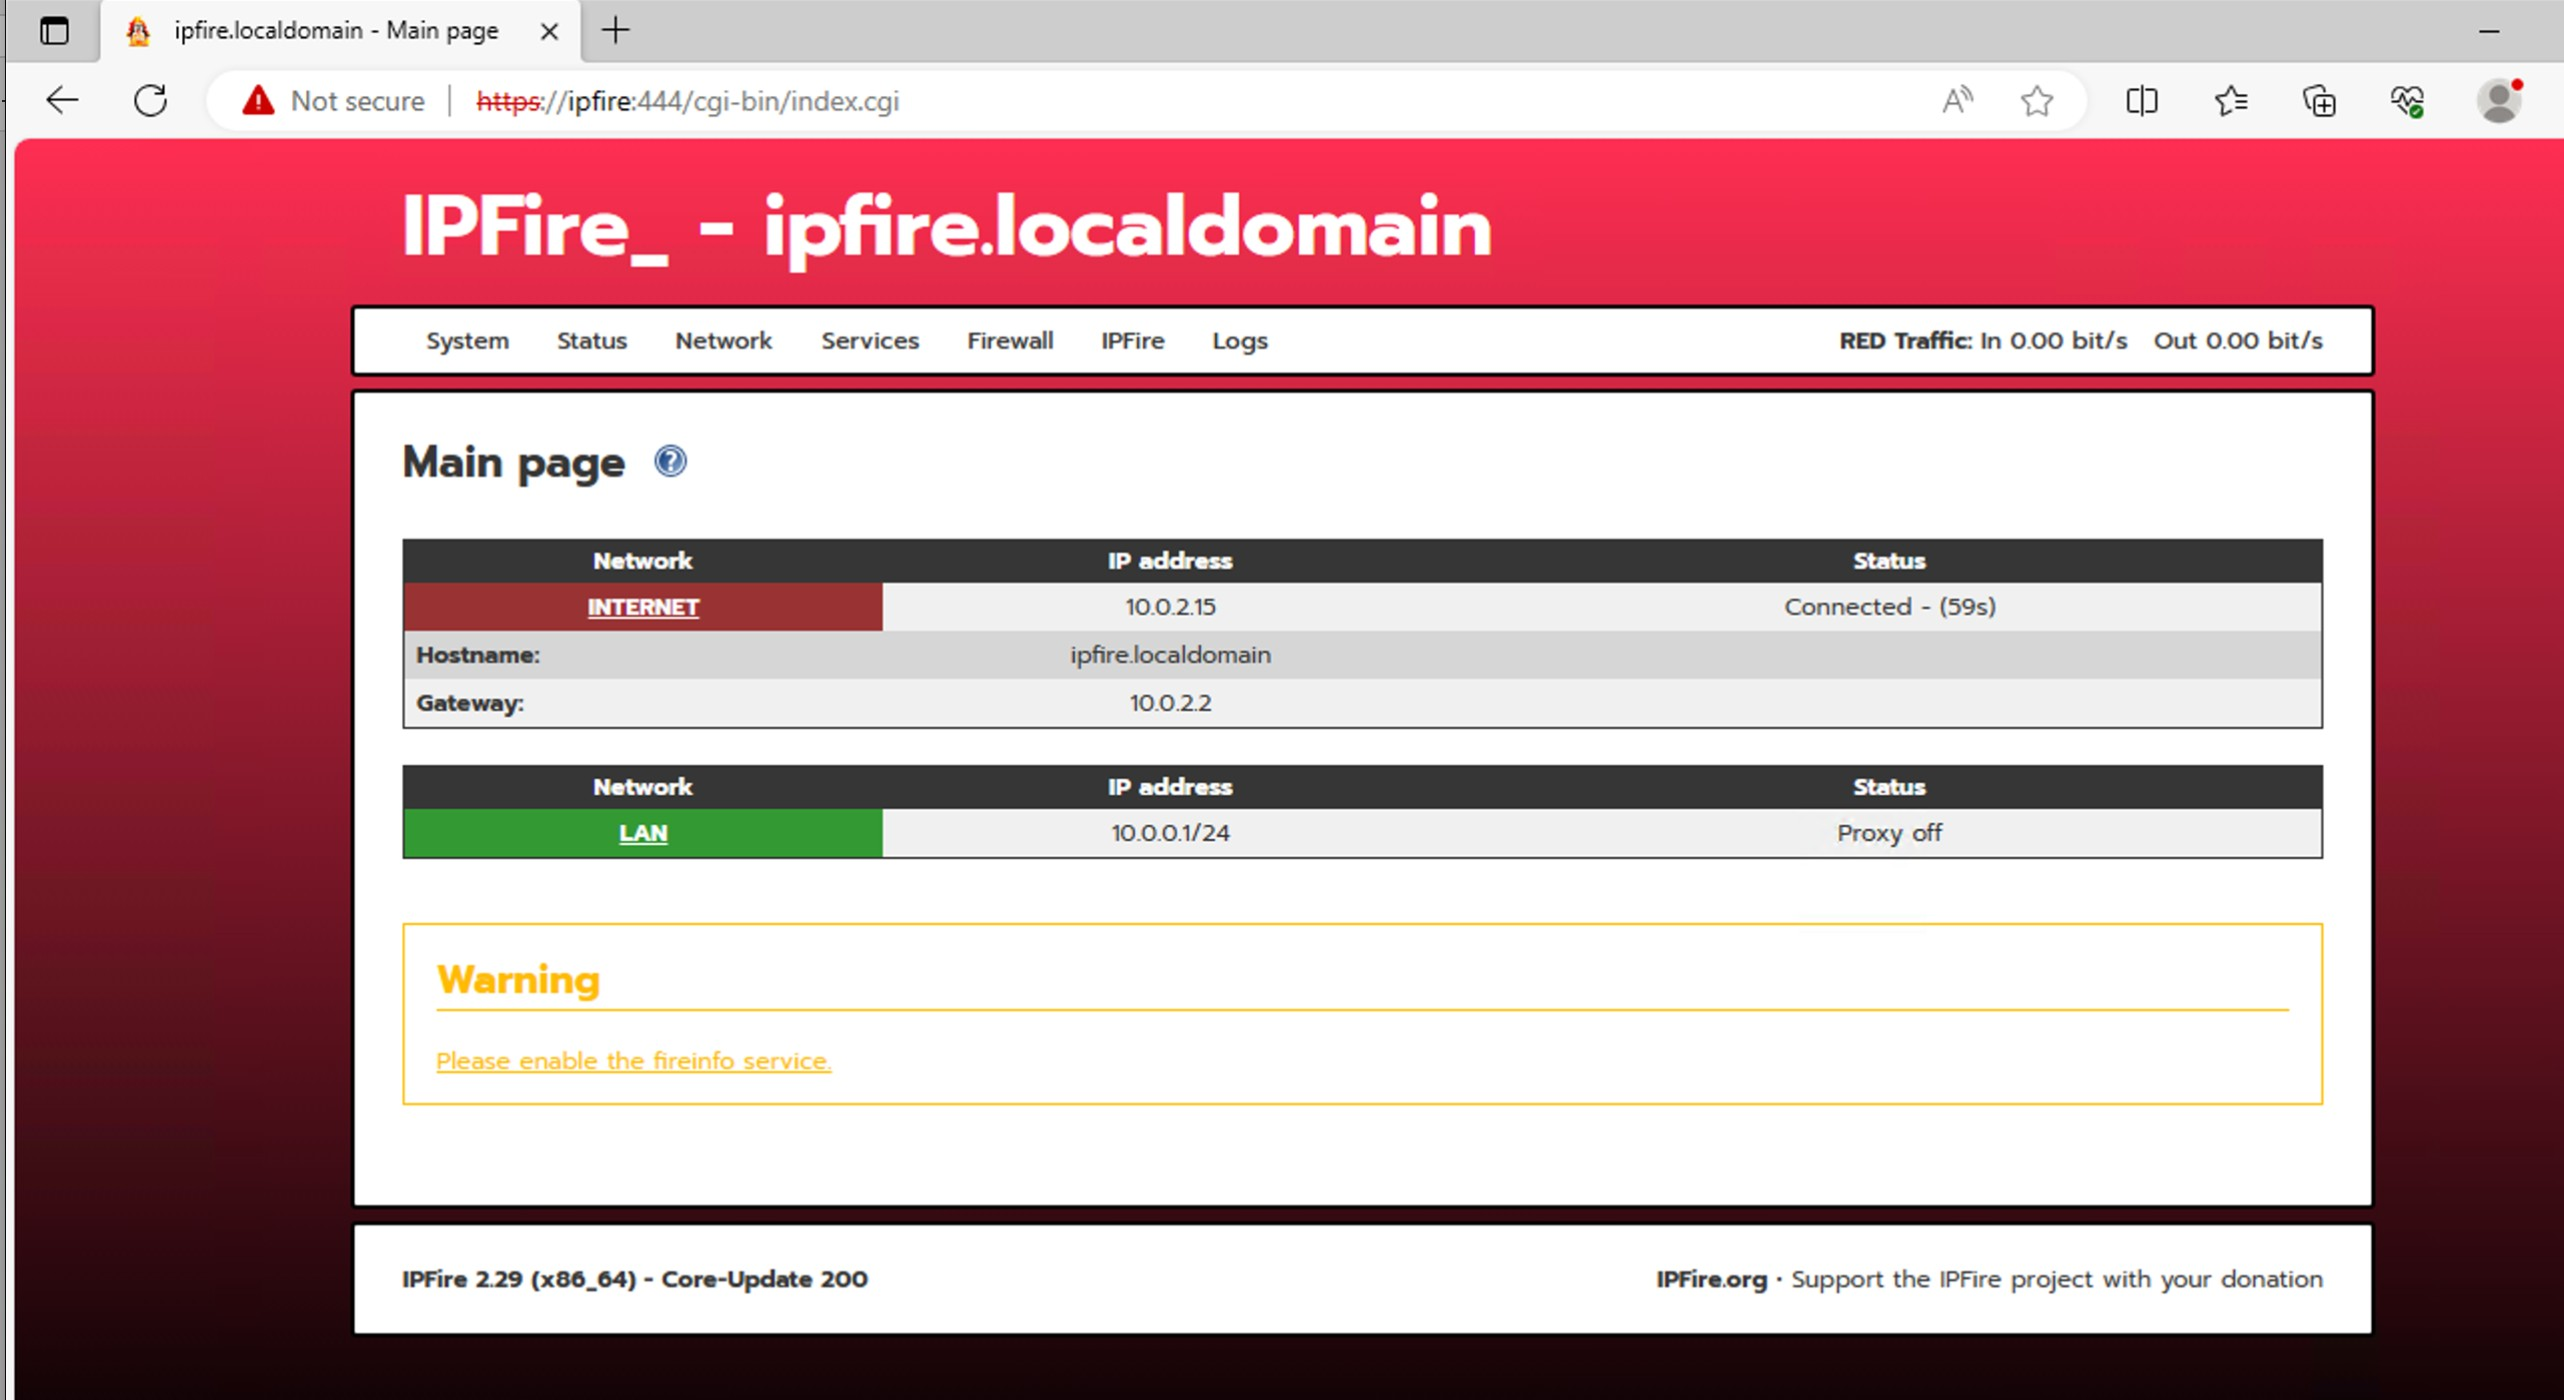
\includegraphics[width=0.9\textwidth]{media/ipfire/12.jpg}
	\caption{Strona domowa pod zakładką System}
	\label{fig:ipf_12}
\end{figure}
\subsubsection{Zakładka Status}
Zawiera wykresy i raportu o zużyciu poszczególnych zasobów systemu, temperaturach itp. [Rys. \ref{fig:ipf_13}]
\begin{figure}[!htbp]
	\centering
	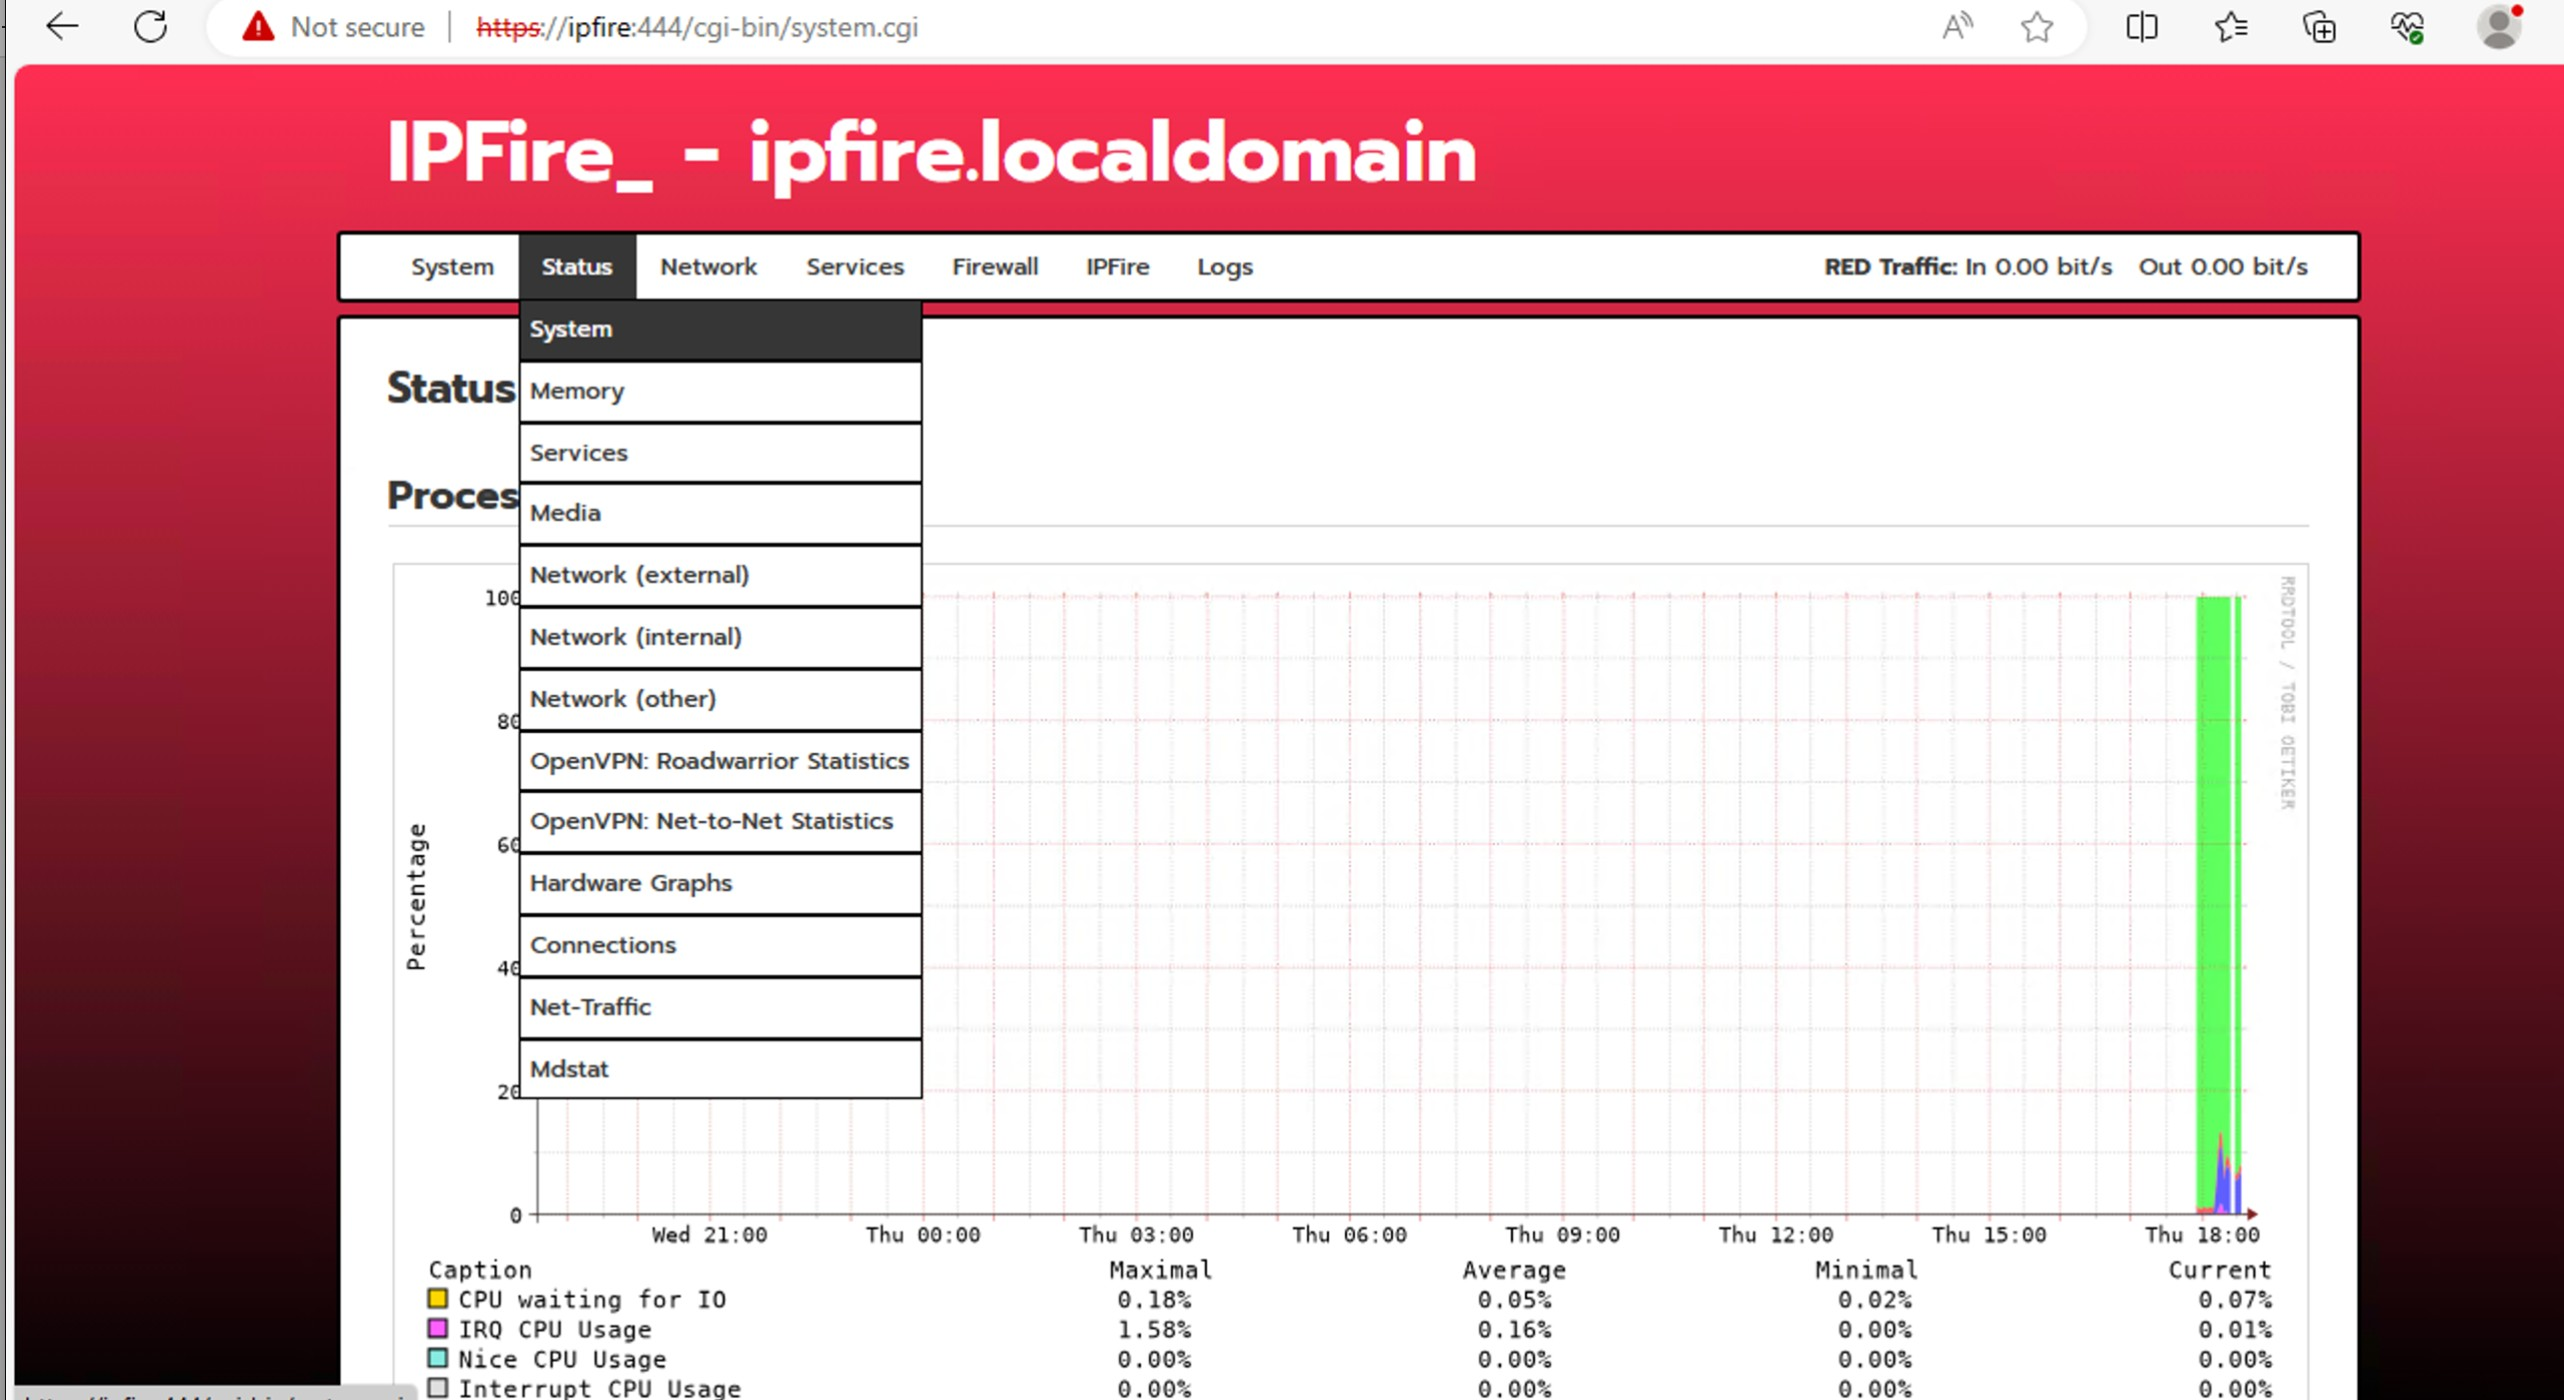
\includegraphics[width=0.9\textwidth]{media/ipfire/13.jpg}
	\caption{Lista Status}
	\label{fig:ipf_13}
\end{figure}
\subsubsection{Zakładka Network}
Zawiera najważniejsze ustawienia i usługi sieciowe, w tym m.in. ustawienia stref, DNS, web proxy, url filtering, DHCP itd. [Rys. \ref{fig:ipf_14}]
\begin{figure}[!htbp]
	\centering
	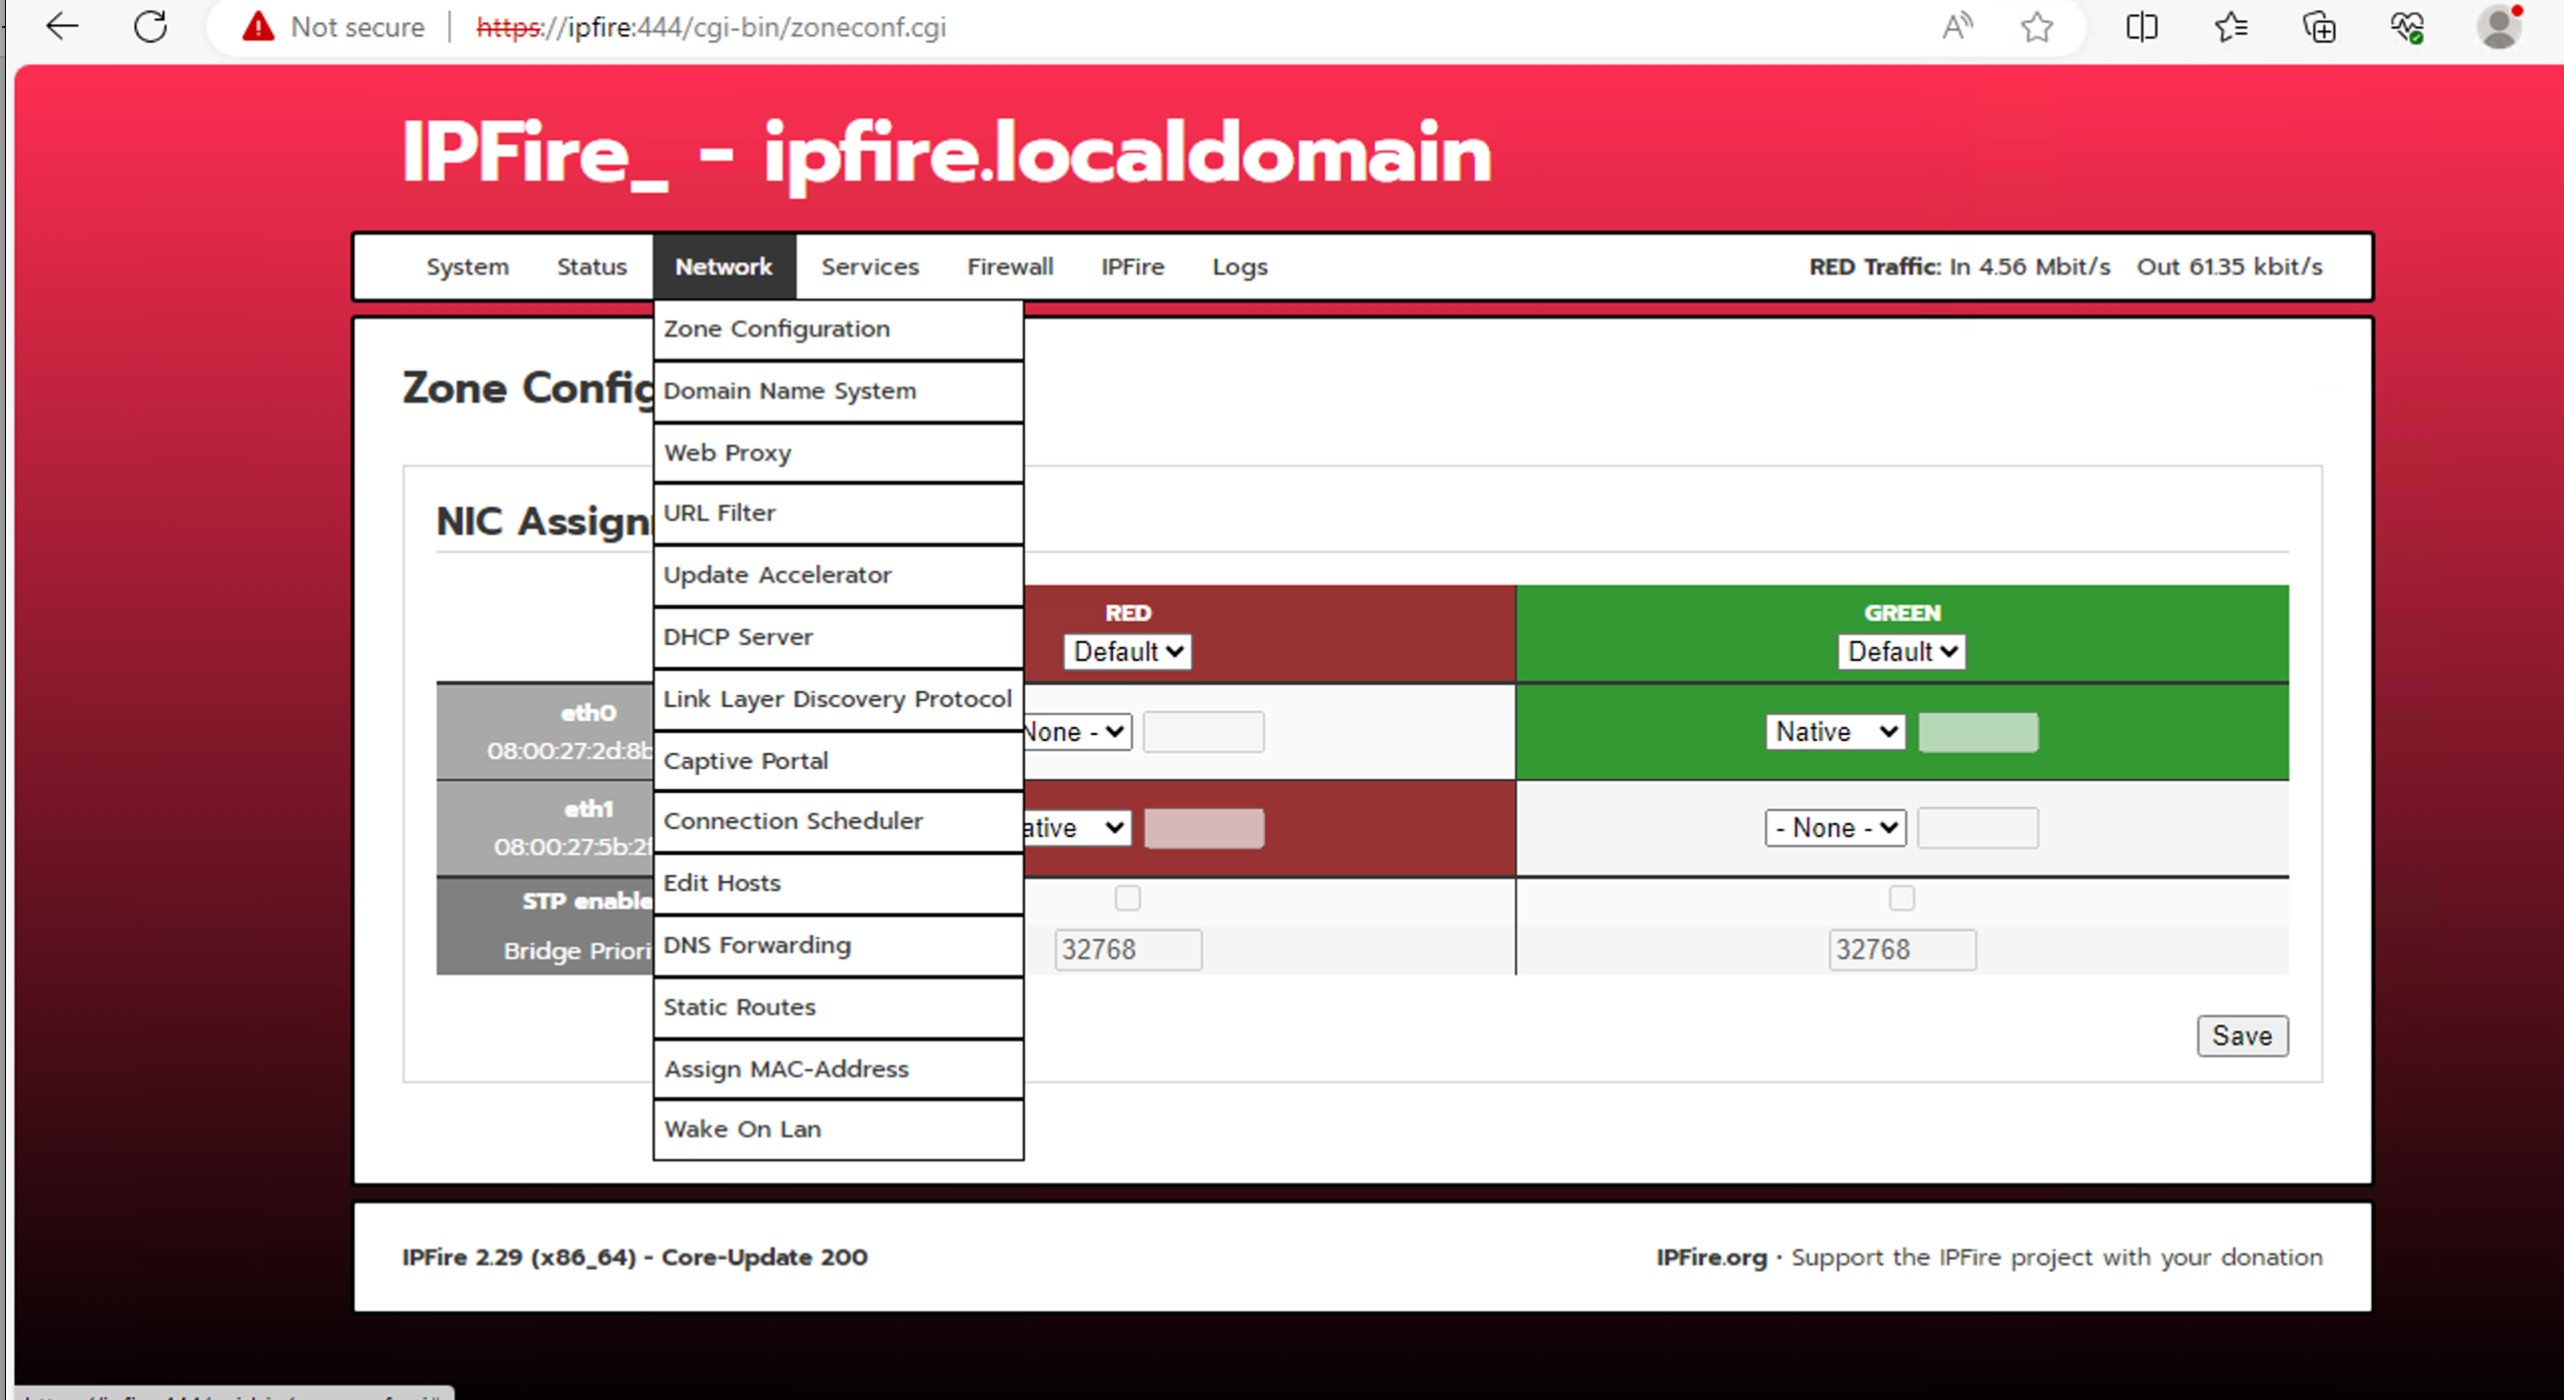
\includegraphics[width=0.9\textwidth]{media/ipfire/14.jpg}
	\caption{Lista Network}
	\label{fig:ipf_14}
\end{figure}
\subsubsection{Zakładka Services}
Usługi zapewniane przez IPFire, w tym QoS i serwery VPN (IPsec, Wireguard, OpenVPN) [Rys. \ref{fig:ipf_15}]
\begin{figure}[!htbp]
	\centering
	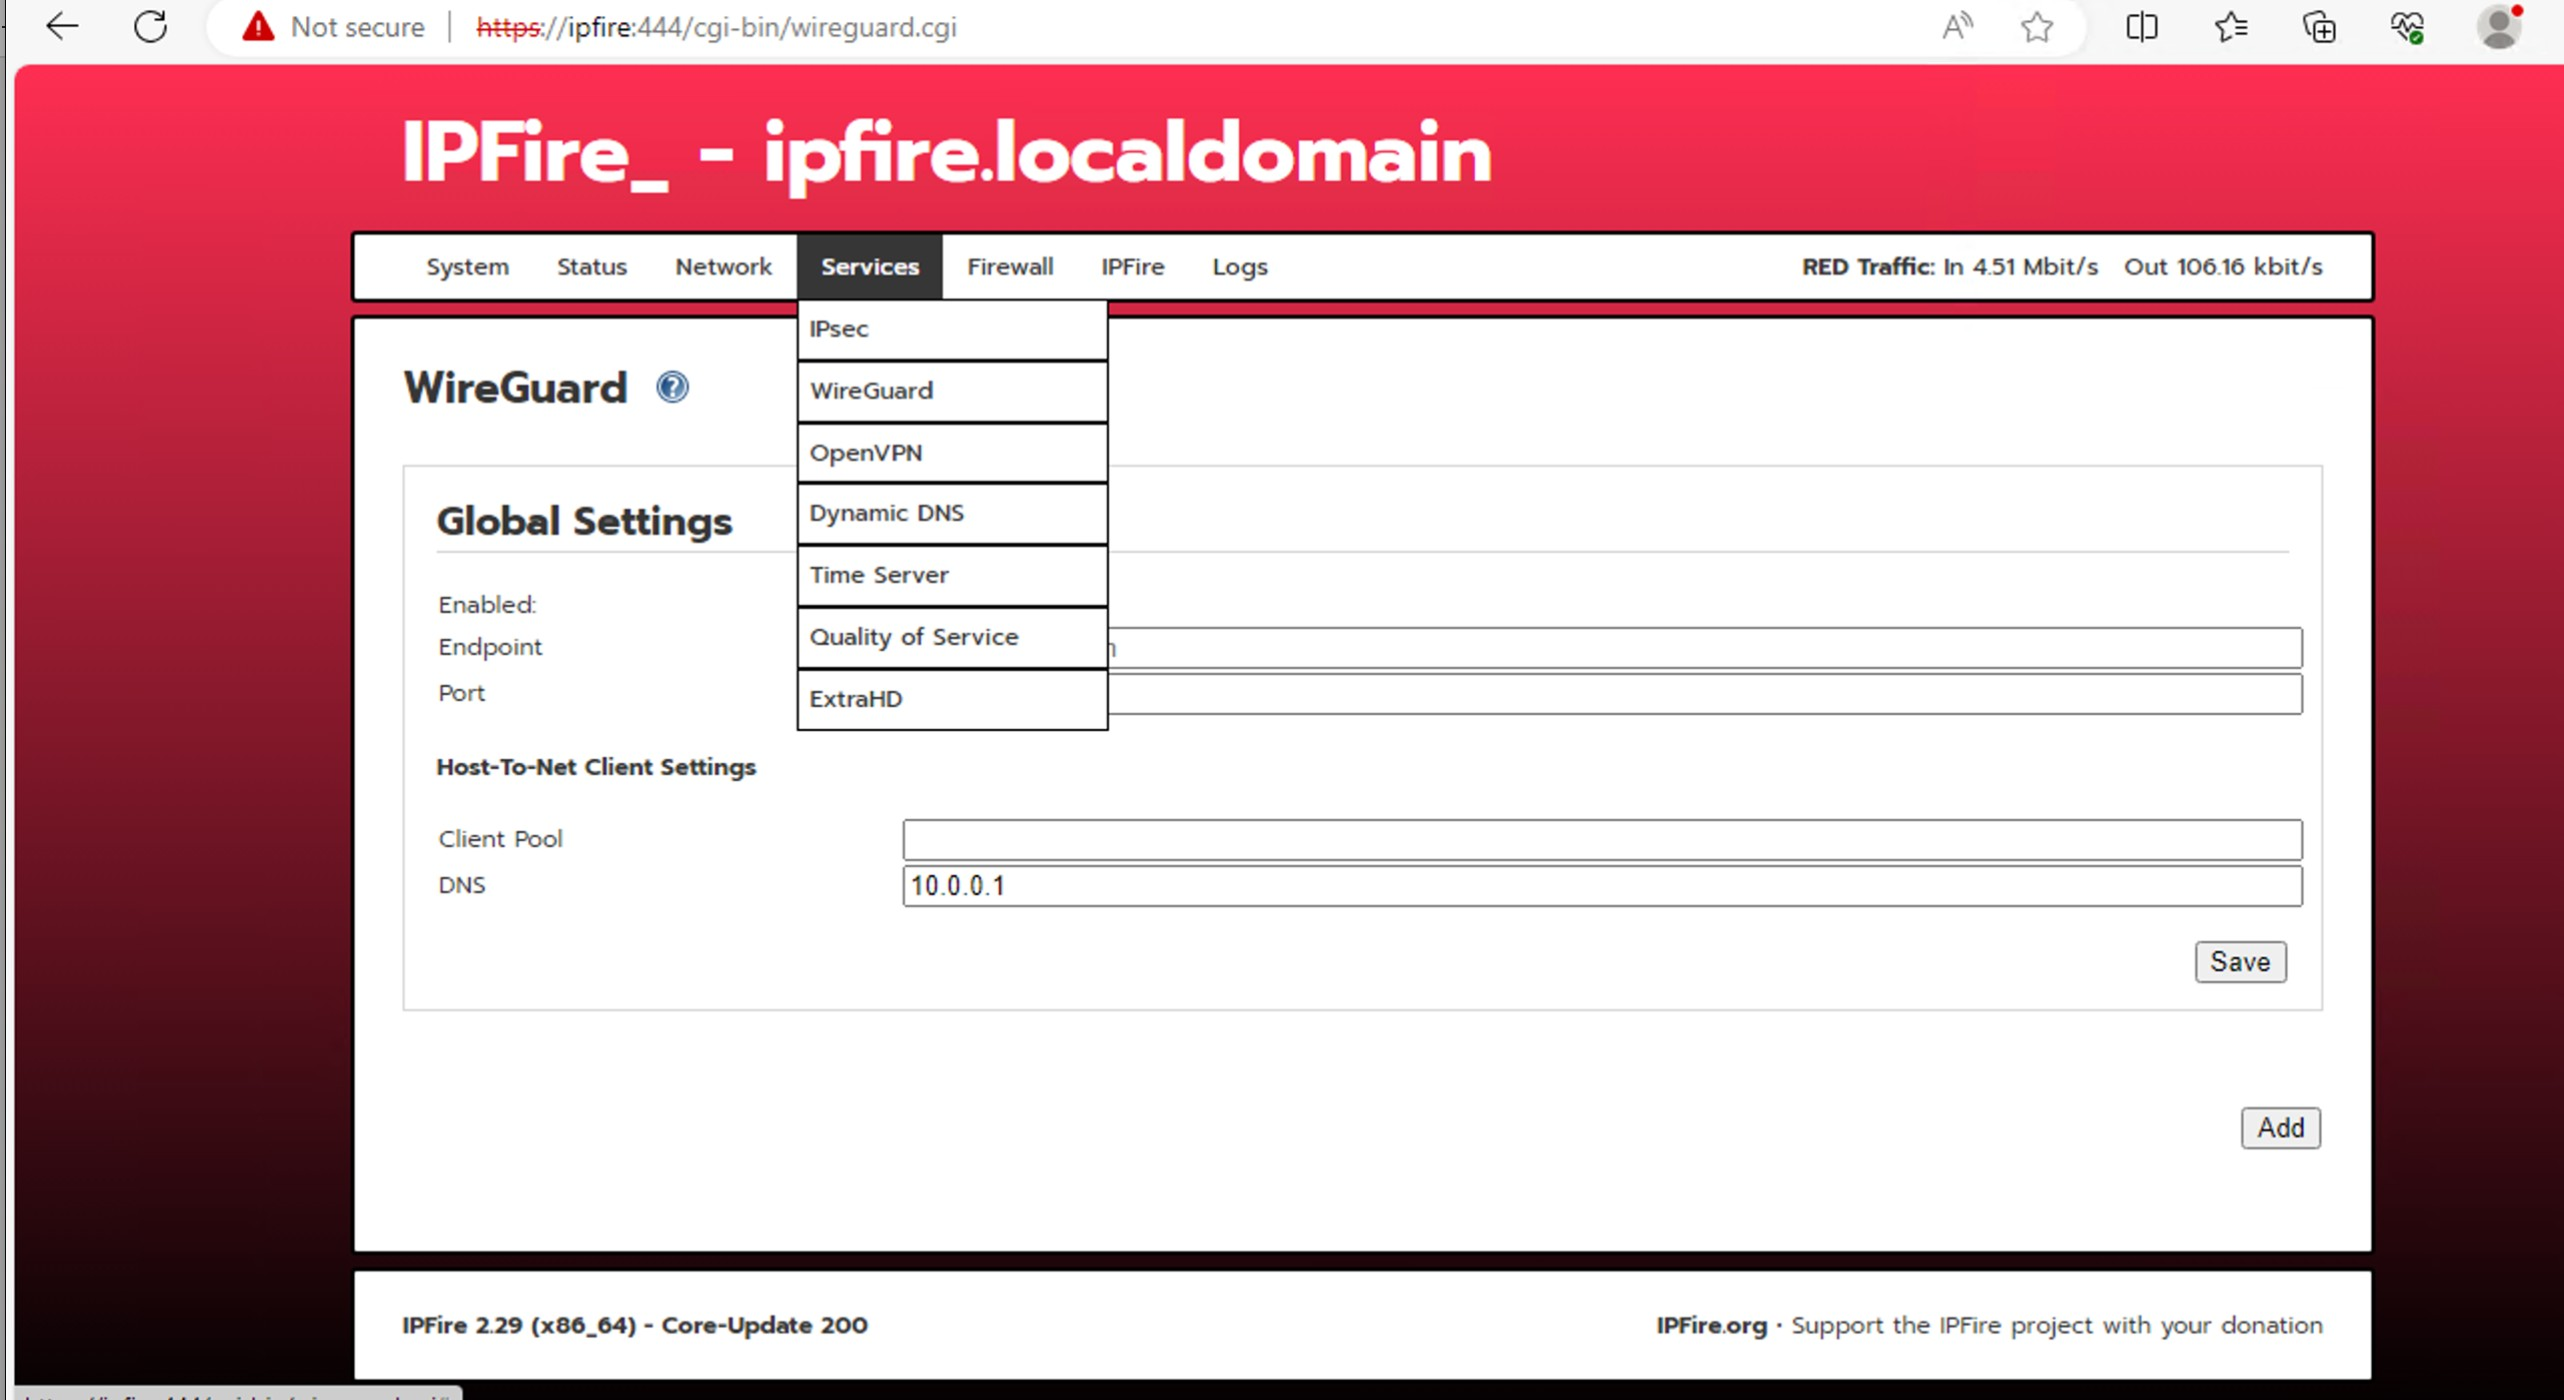
\includegraphics[width=0.9\textwidth]{media/ipfire/15.jpg}
	\caption{Lista Services}
	\label{fig:ipf_15}
\end{figure}
\subsubsection{Zakładka Firewall}
Wszystkie ustawienia związane z zaporą sieciową - reguły, grupy, geolokalizacja, blokowanie według list IP, konfiguracja IPS. [Rys. \ref{fig:ipf_16}]
\begin{figure}[!htbp]
	\centering
	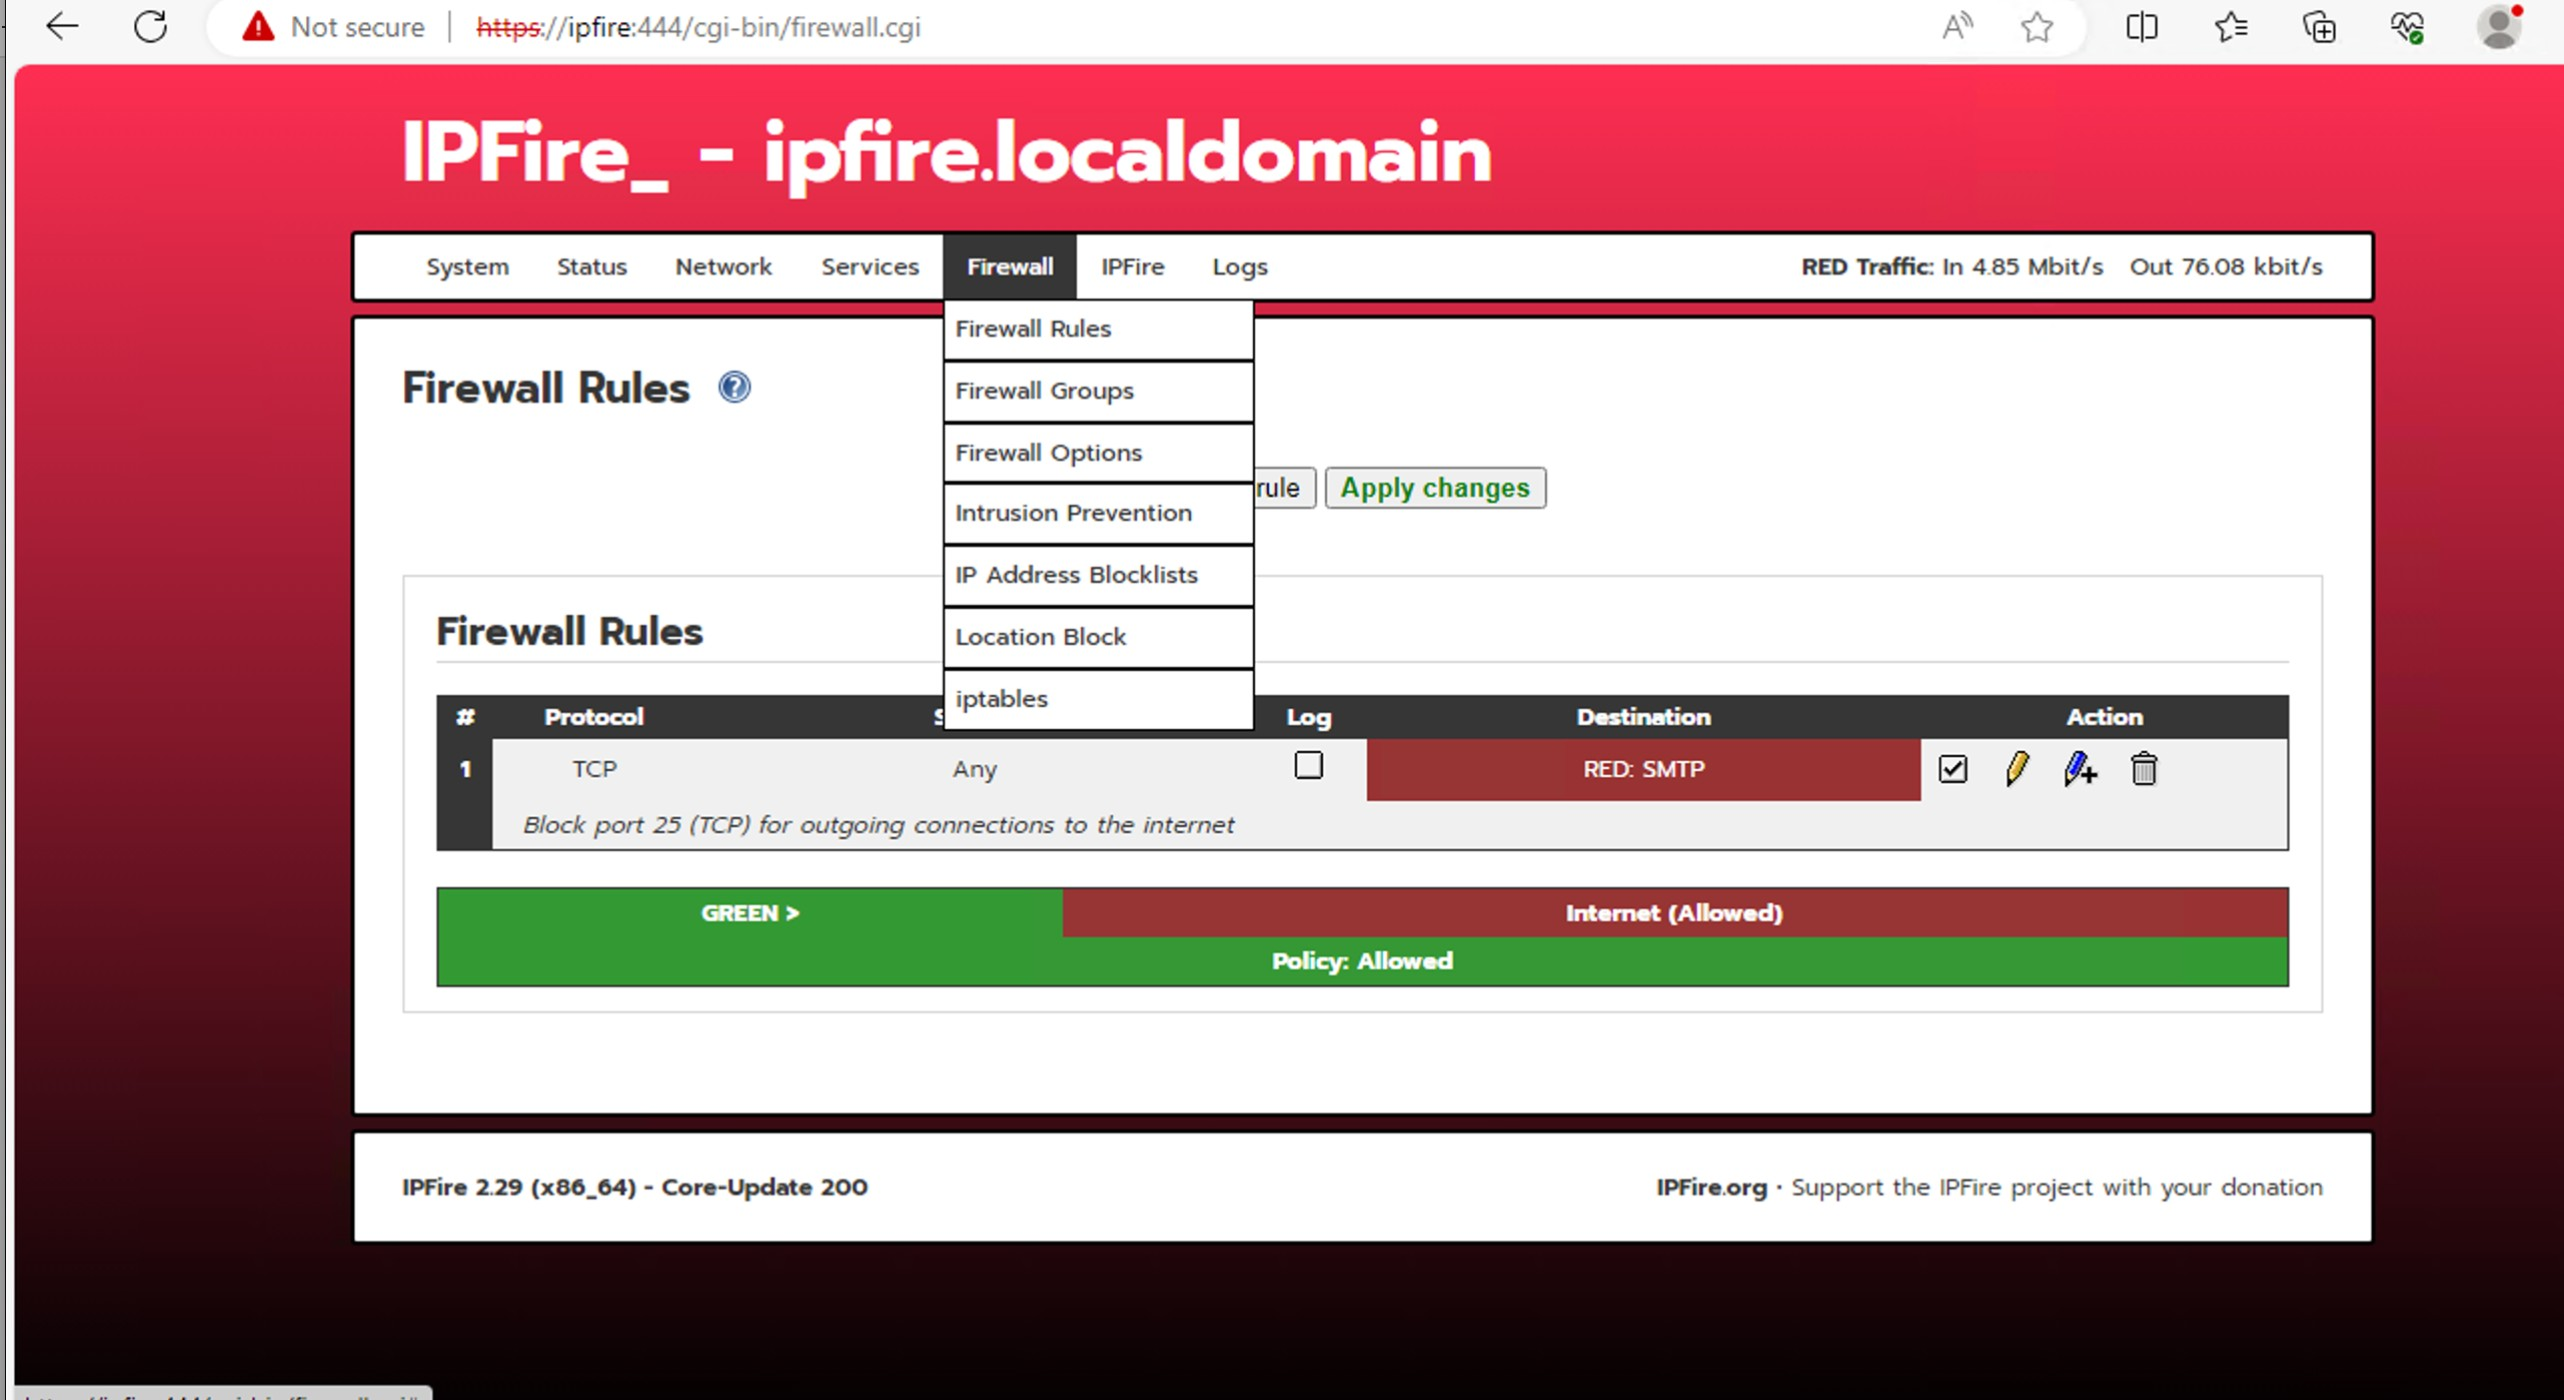
\includegraphics[width=0.9\textwidth]{media/ipfire/16.jpg}
	\caption{Lista Firewall}
	\label{fig:ipf_16}
\end{figure}
\subsubsection{Zakładka IPFire}
Zarządzanie pakietami przez menedżer Pakfire.
\subsubsection{Zakładka Logs}
Wyświetlanie różnego rodzaju logów generowanych przez system, firewall, system IPS, VPN itd.

\subsection{Konfiguracja przykładowej funkcjonalności - filtrowania URL}
Aby móc filtrować strony po URL, należy najpierw uruchomić usługę Web Proxy. W Network->Web Proxy zaznaczamy opcje "Enabled on Green" oraz "URL filter: Enabled". Warto włączyć też zbieranie logów [Rys. \ref{fig:ipf_17}]
\begin{figure}[!htbp]
	\centering
	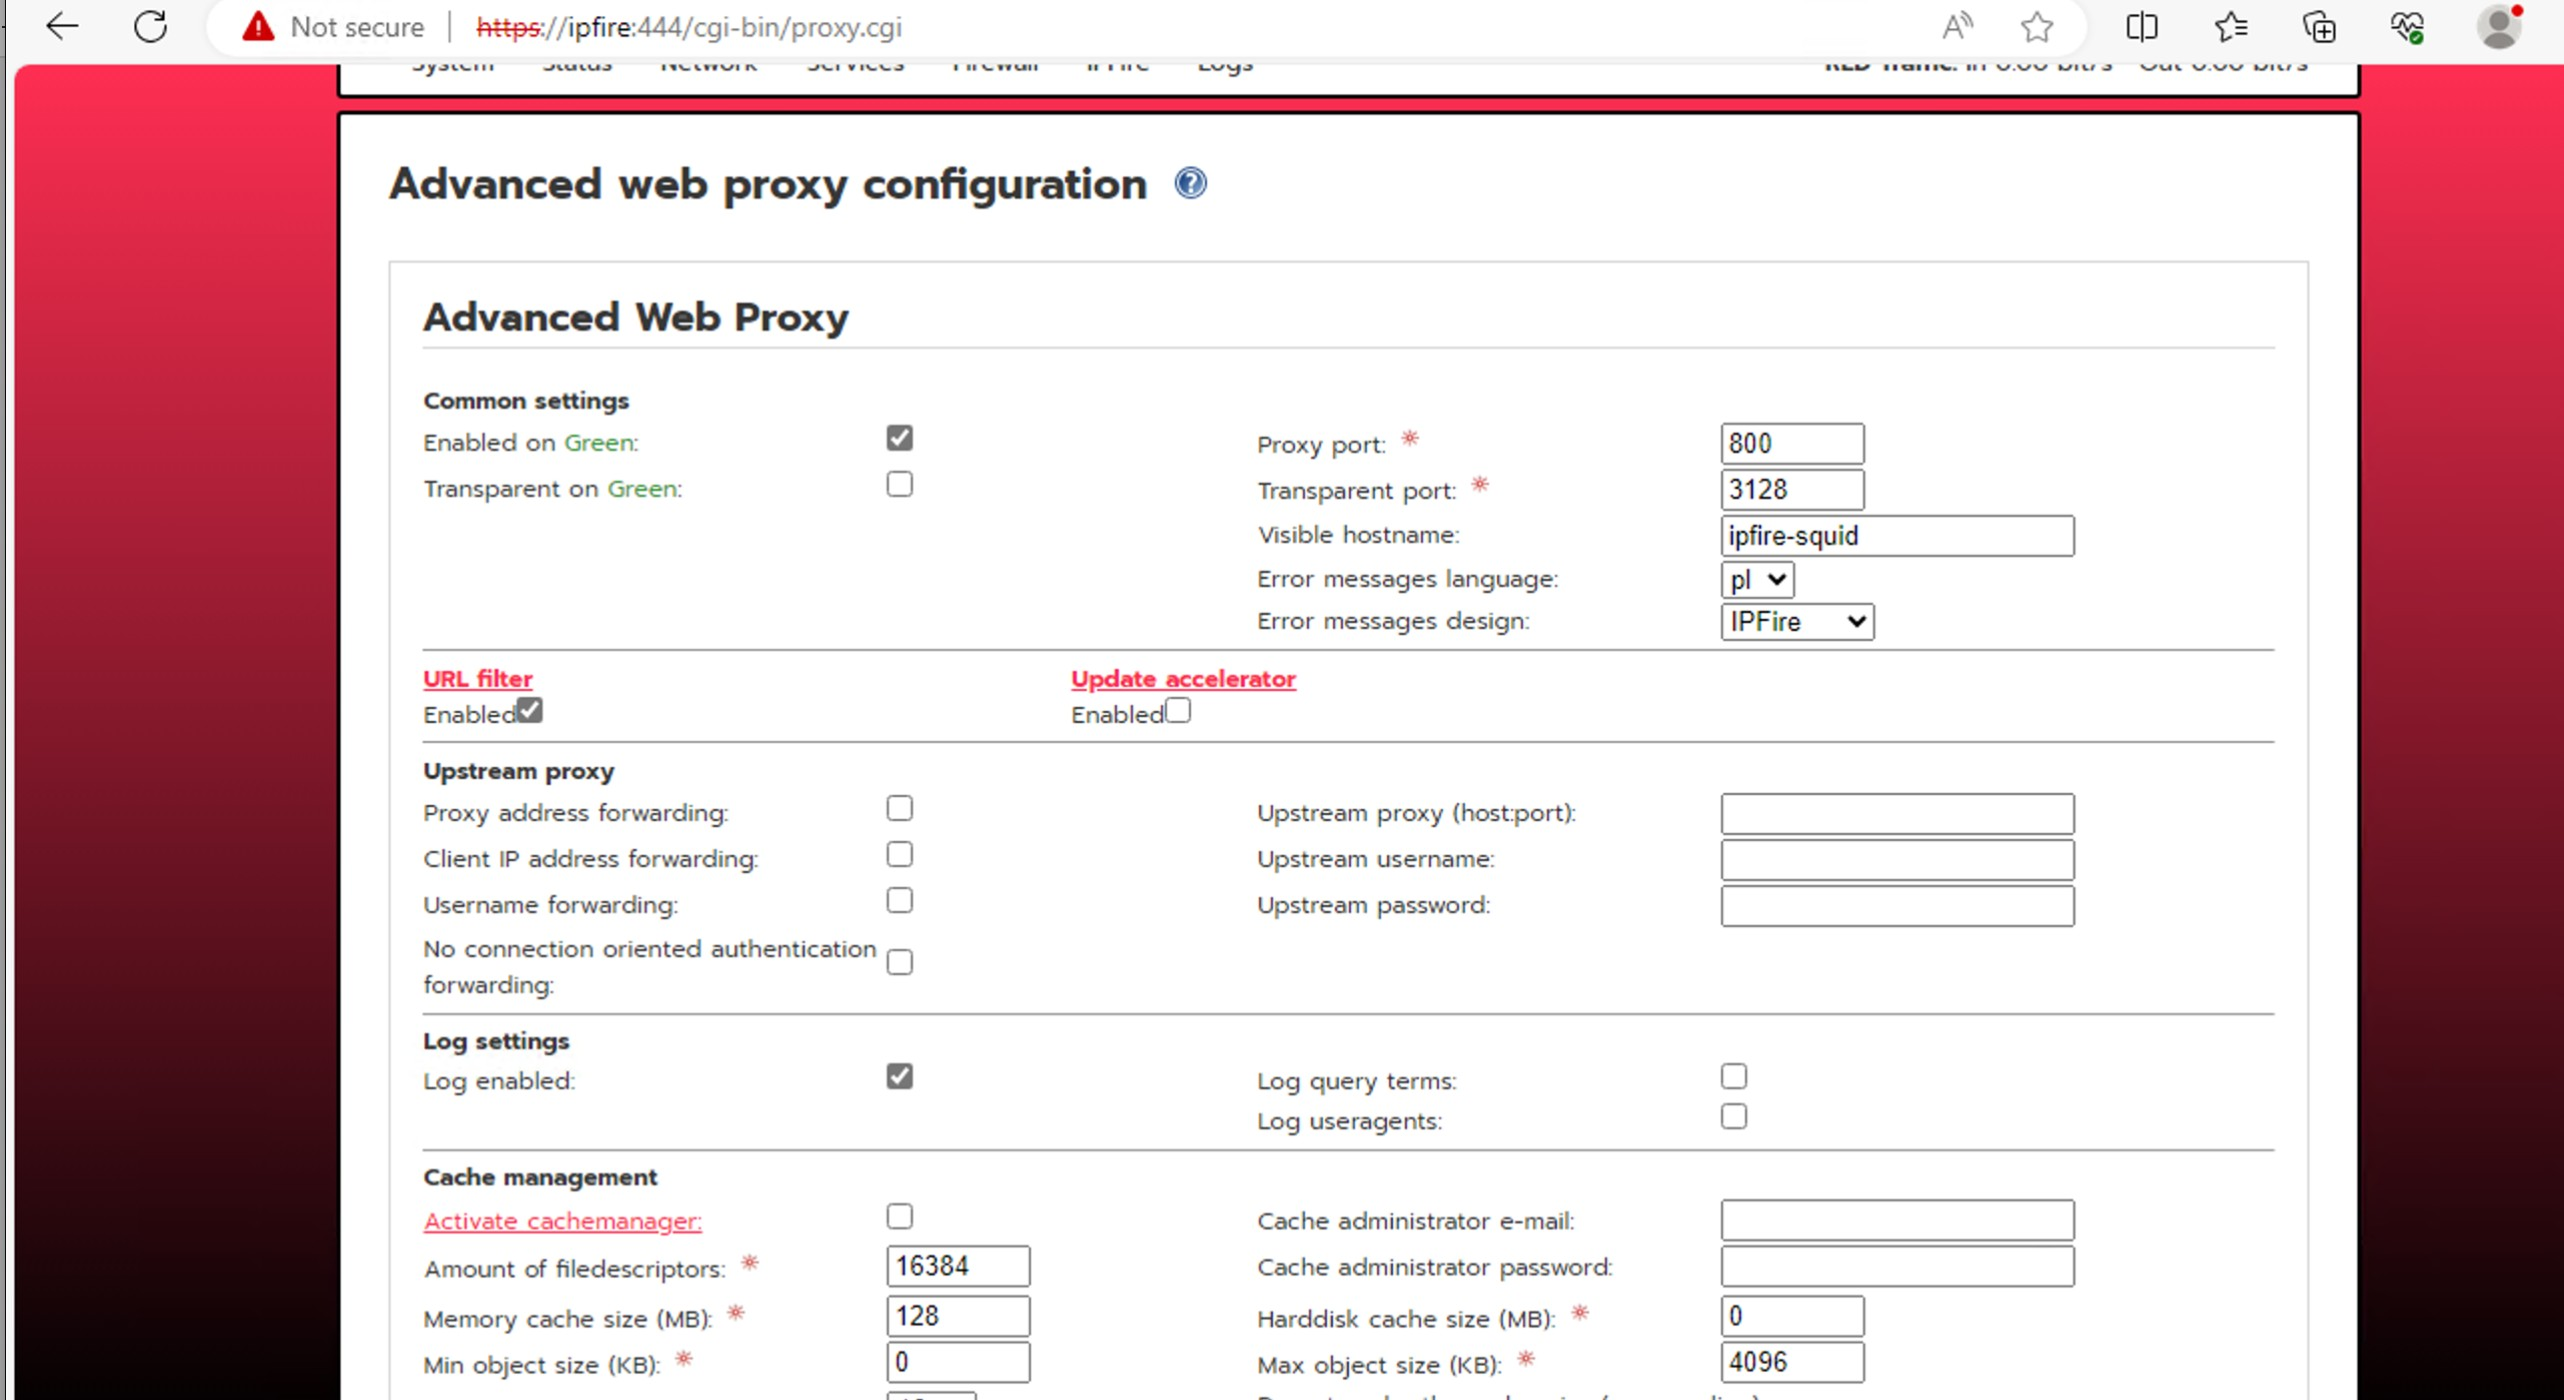
\includegraphics[width=0.9\textwidth]{media/ipfire/17.jpg}
	\caption{Konfiguracja Web Proxy}
	\label{fig:ipf_17}
\end{figure}

Następnie należy ustawić blokowanie ruchu typu "Forward" aby zapobiec przechodzeniu ruchu poza Proxy. W Firewall->Firewall Options->Default firewall behaviour wybieramy z listy "Blocked" pod sekcją "Forward" [Rys. \ref{fig:ipf_18}]
\begin{figure}[!htbp]
	\centering
	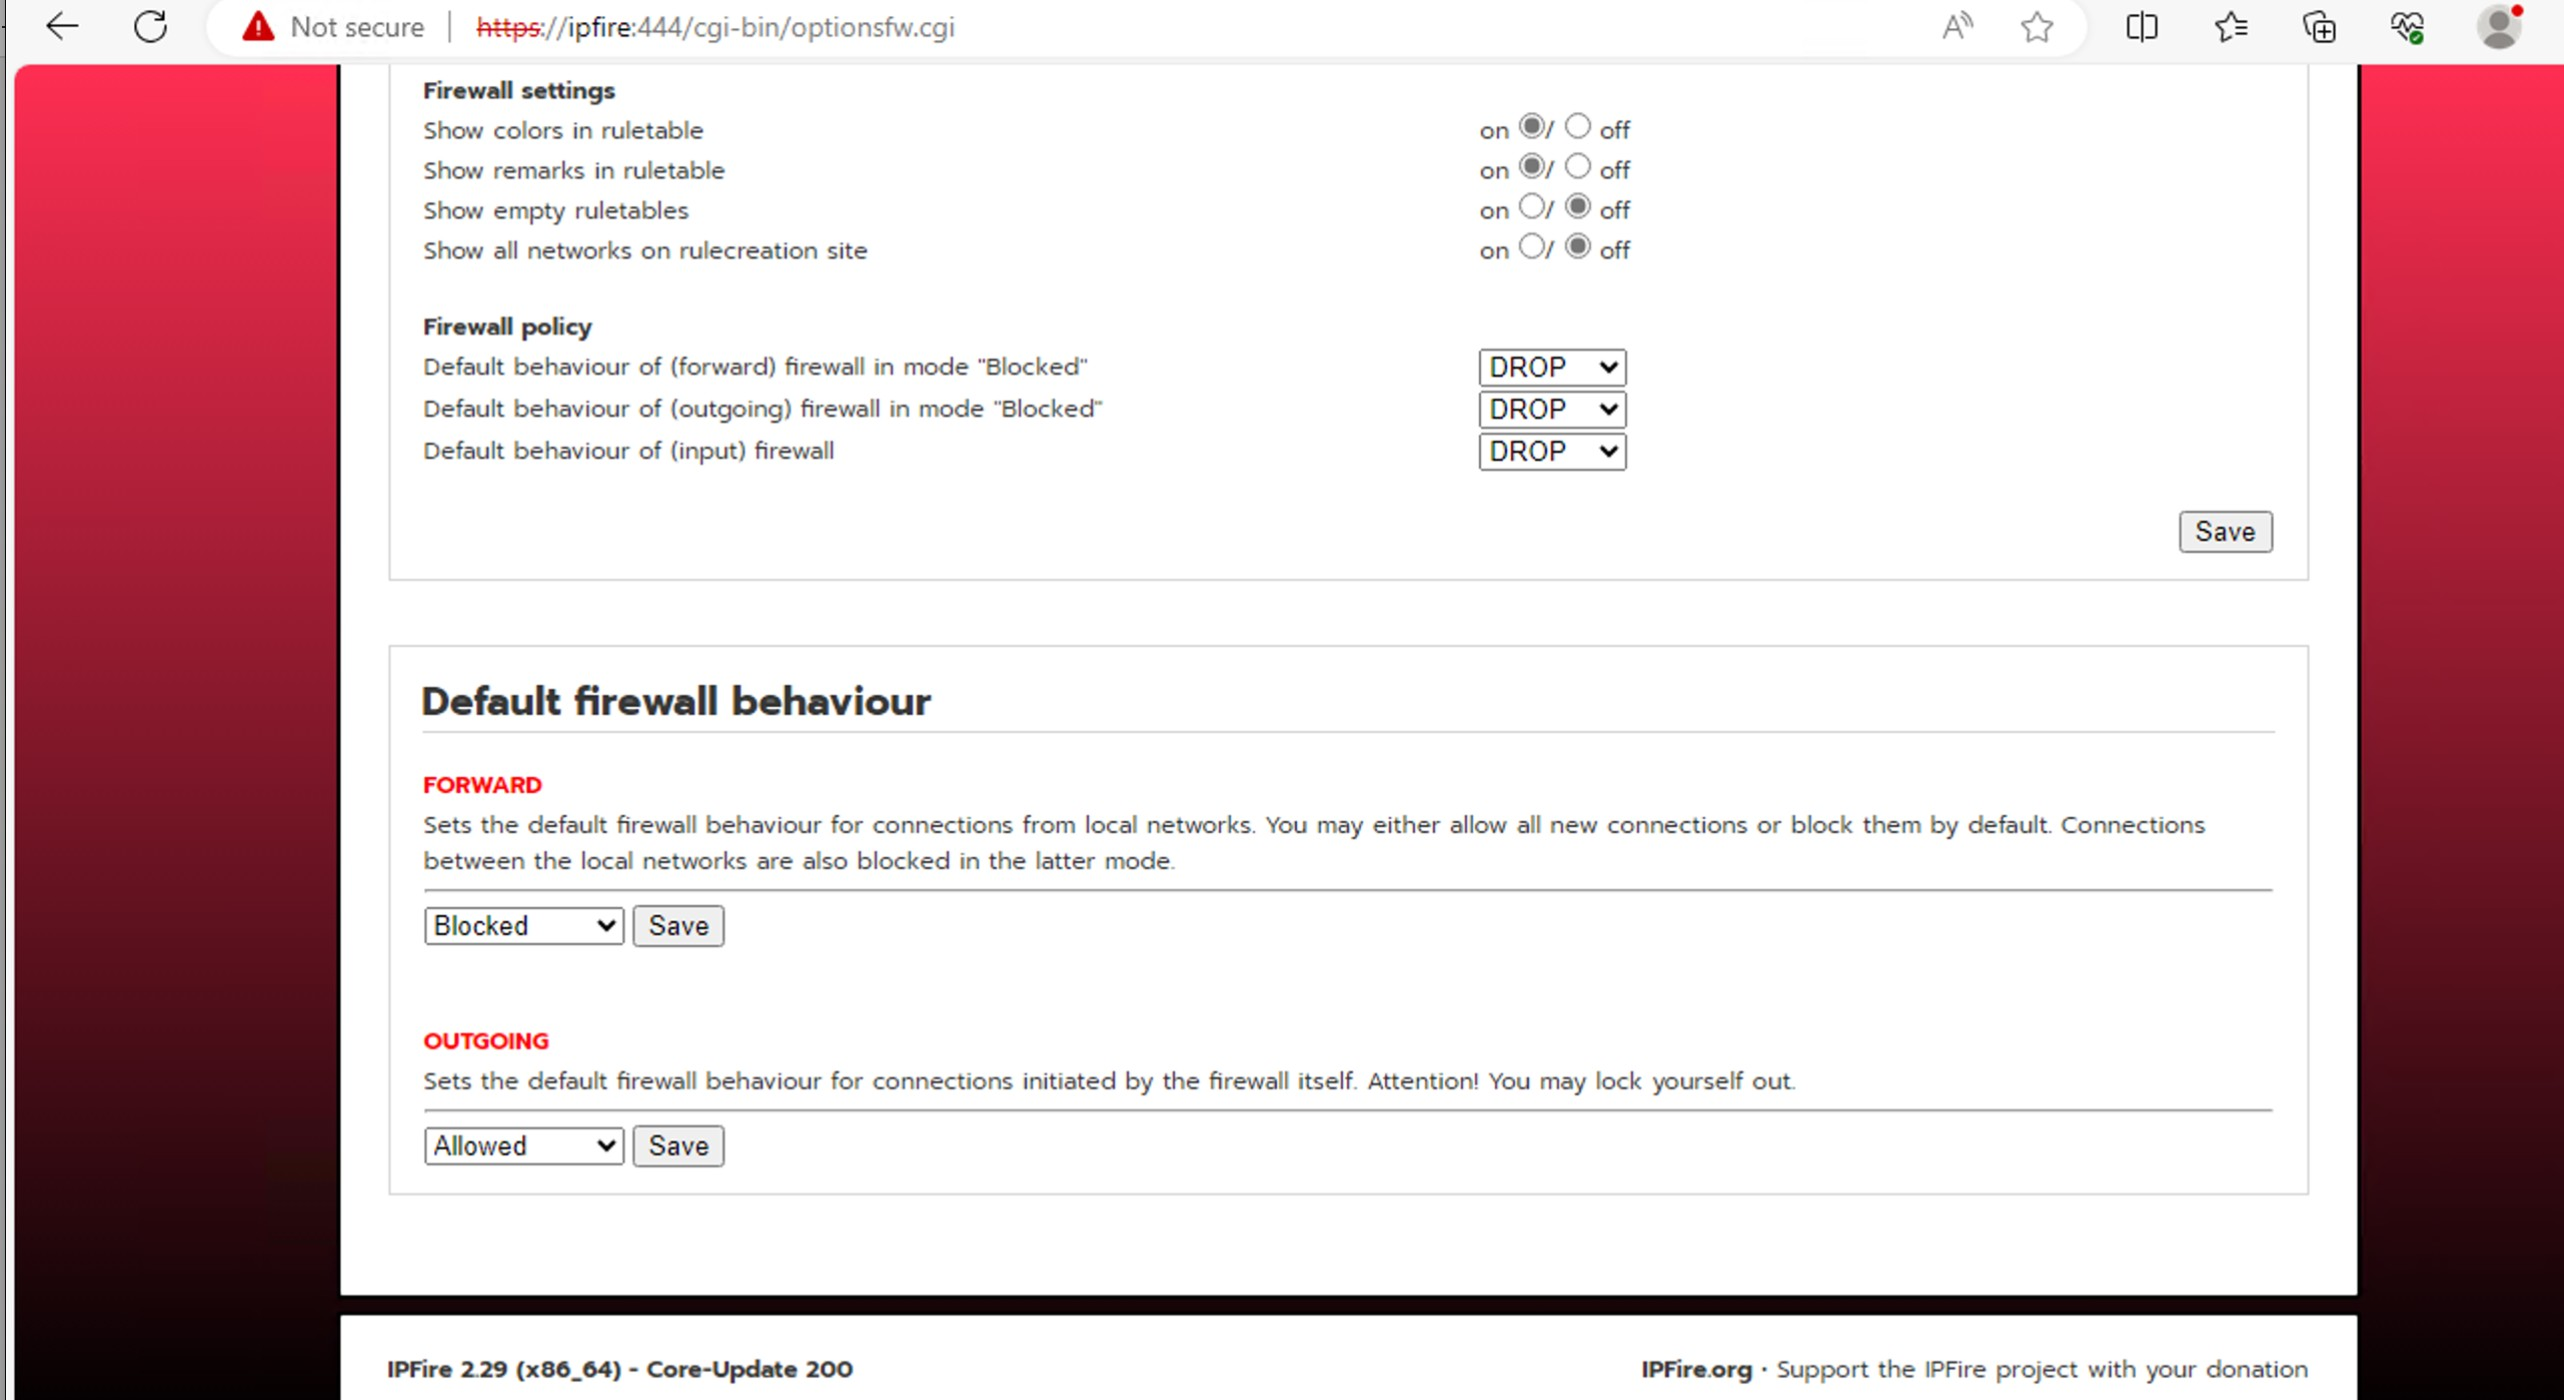
\includegraphics[width=0.9\textwidth]{media/ipfire/18.jpg}
	\caption{Konfiguracja Default Firewall Behaviour}
	\label{fig:ipf_18}
\end{figure}

System operacyjny lub przeglądarka powinna mieć skonfigurowane połączenie do serwera Proxy [Rys. \ref{fig:ipf_19}]
\begin{figure}[!htbp]
	\centering
	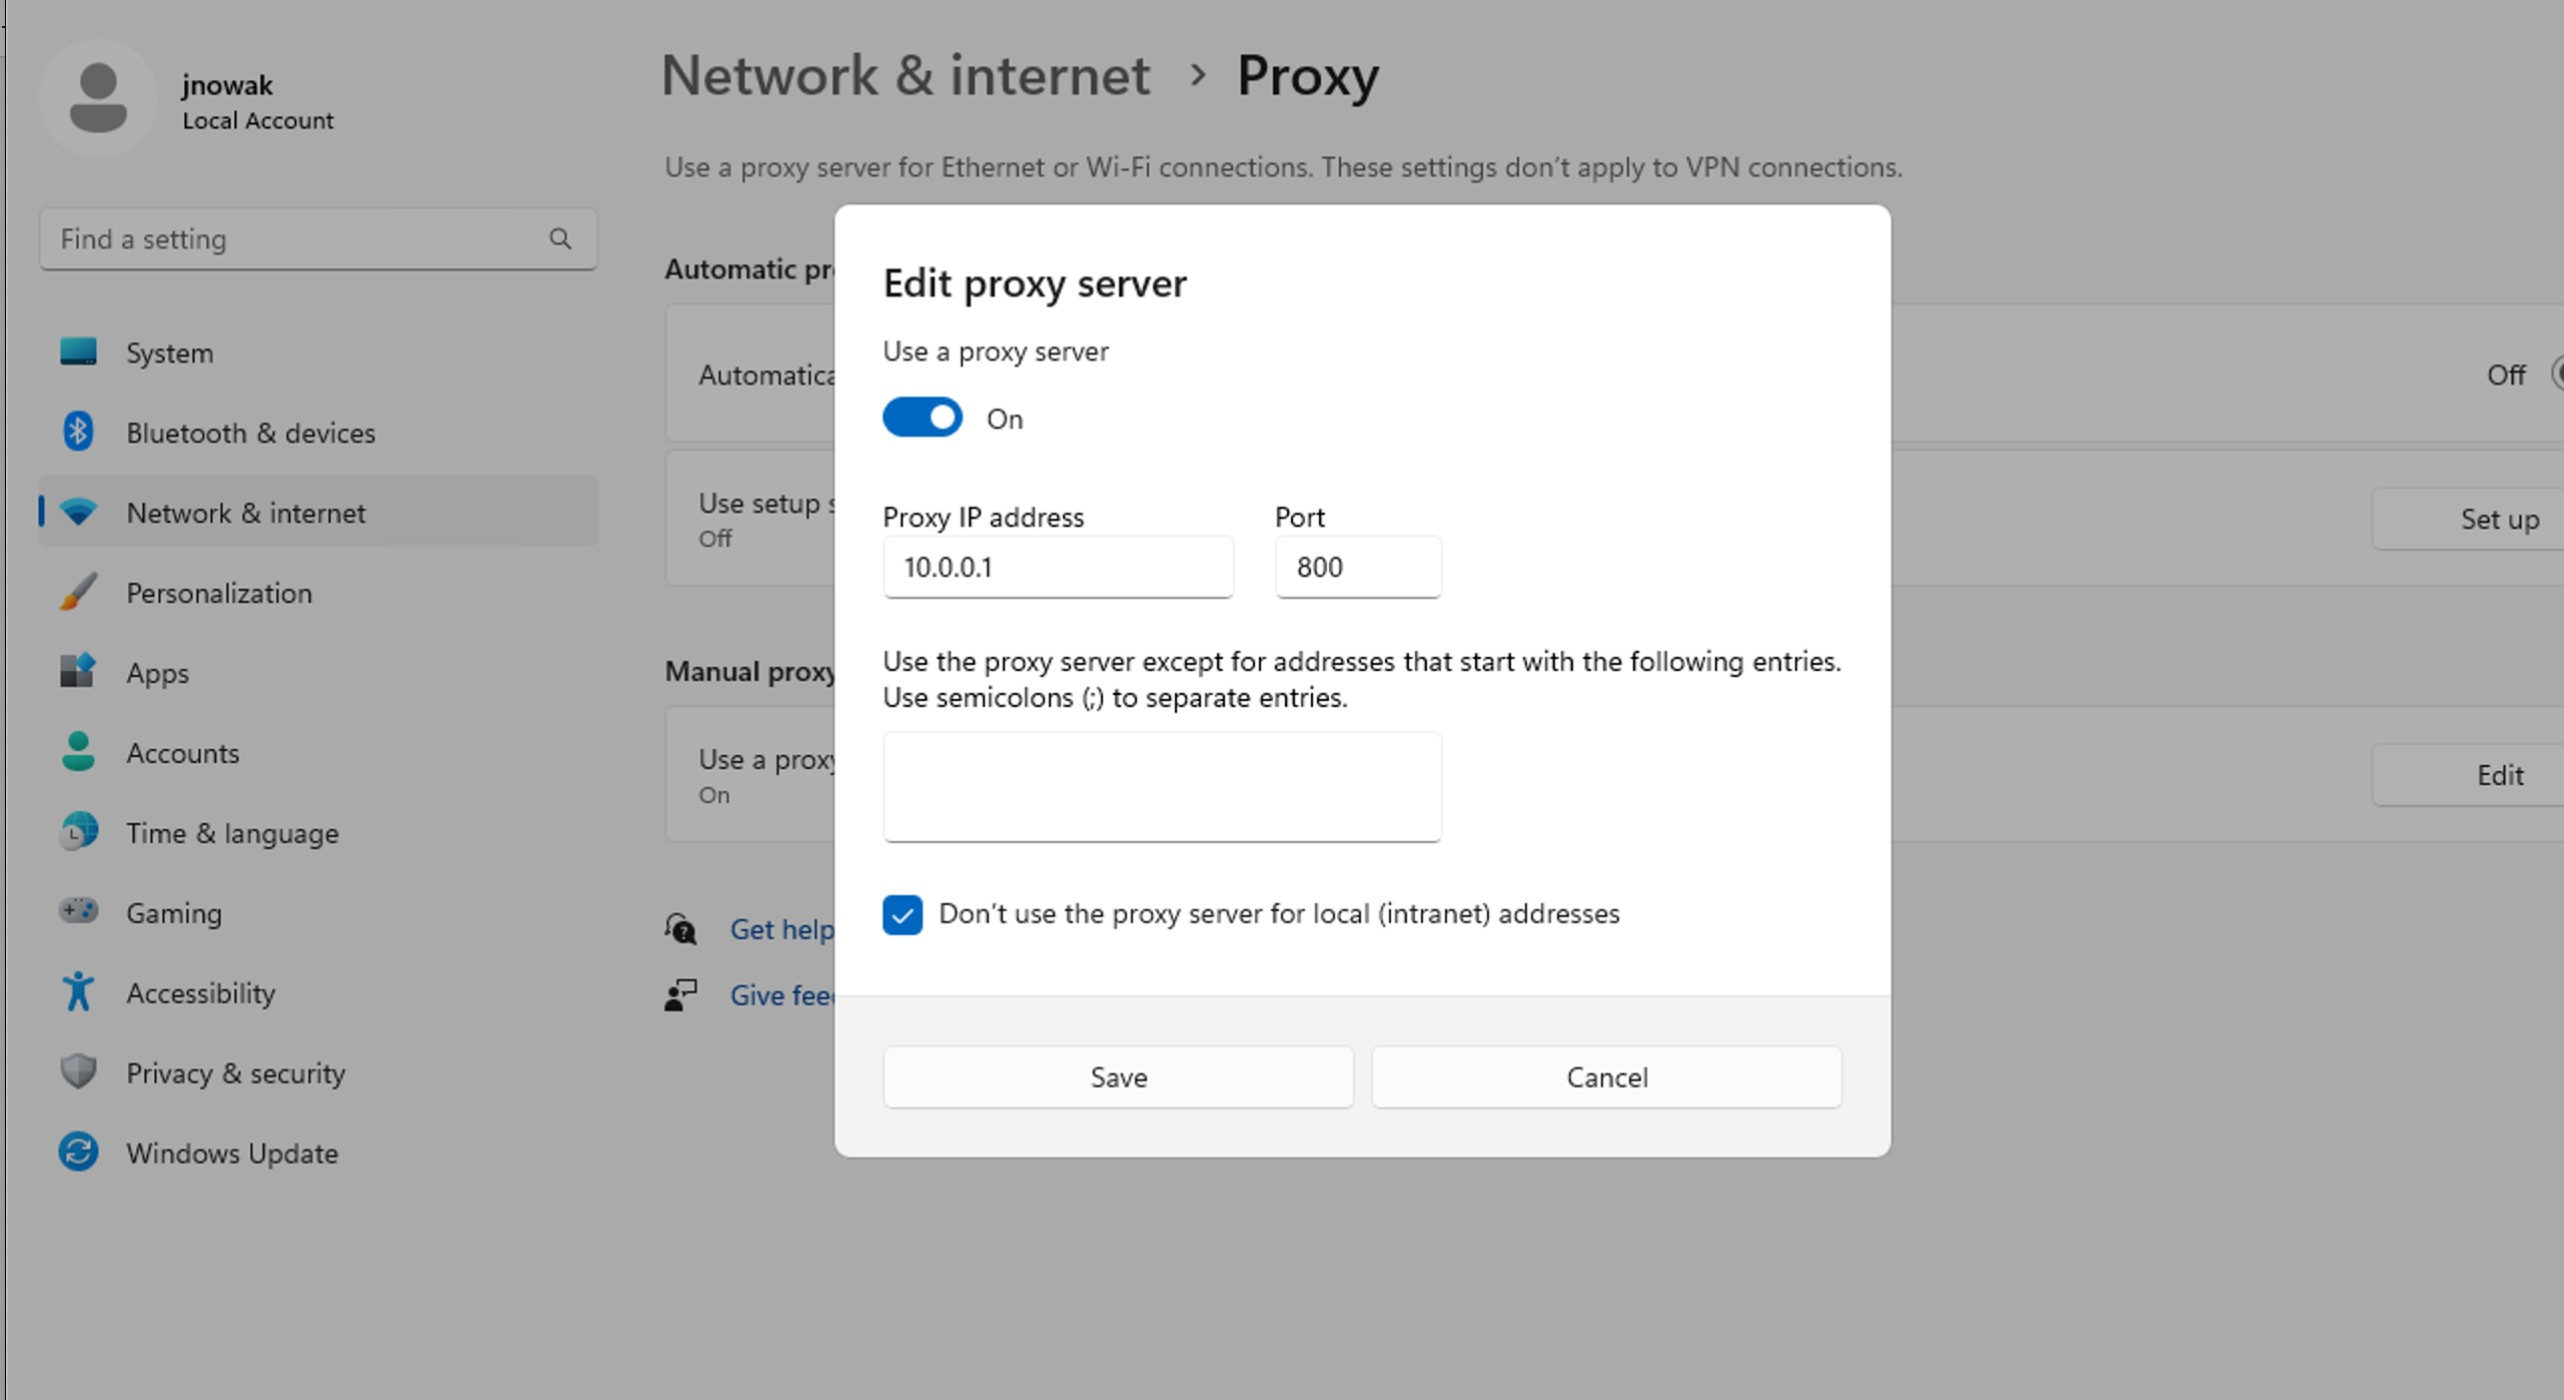
\includegraphics[width=0.9\textwidth]{media/ipfire/19.jpg}
	\caption{Konfiguracja Proxy w systemie klienckim}
	\label{fig:ipf_19}
\end{figure}

Wreszcie można skonfigurować sam URL Filter pod listą Network. W pierwszej kolejności należy zaktualizować domyślną listę domen IPFire DBL (poprzez kliknięcie przycisku "Update now" w sekcji "URL filter maintenance" [Rys. \ref{fig:ipf_20}])
\begin{figure}[!htbp]
	\centering
	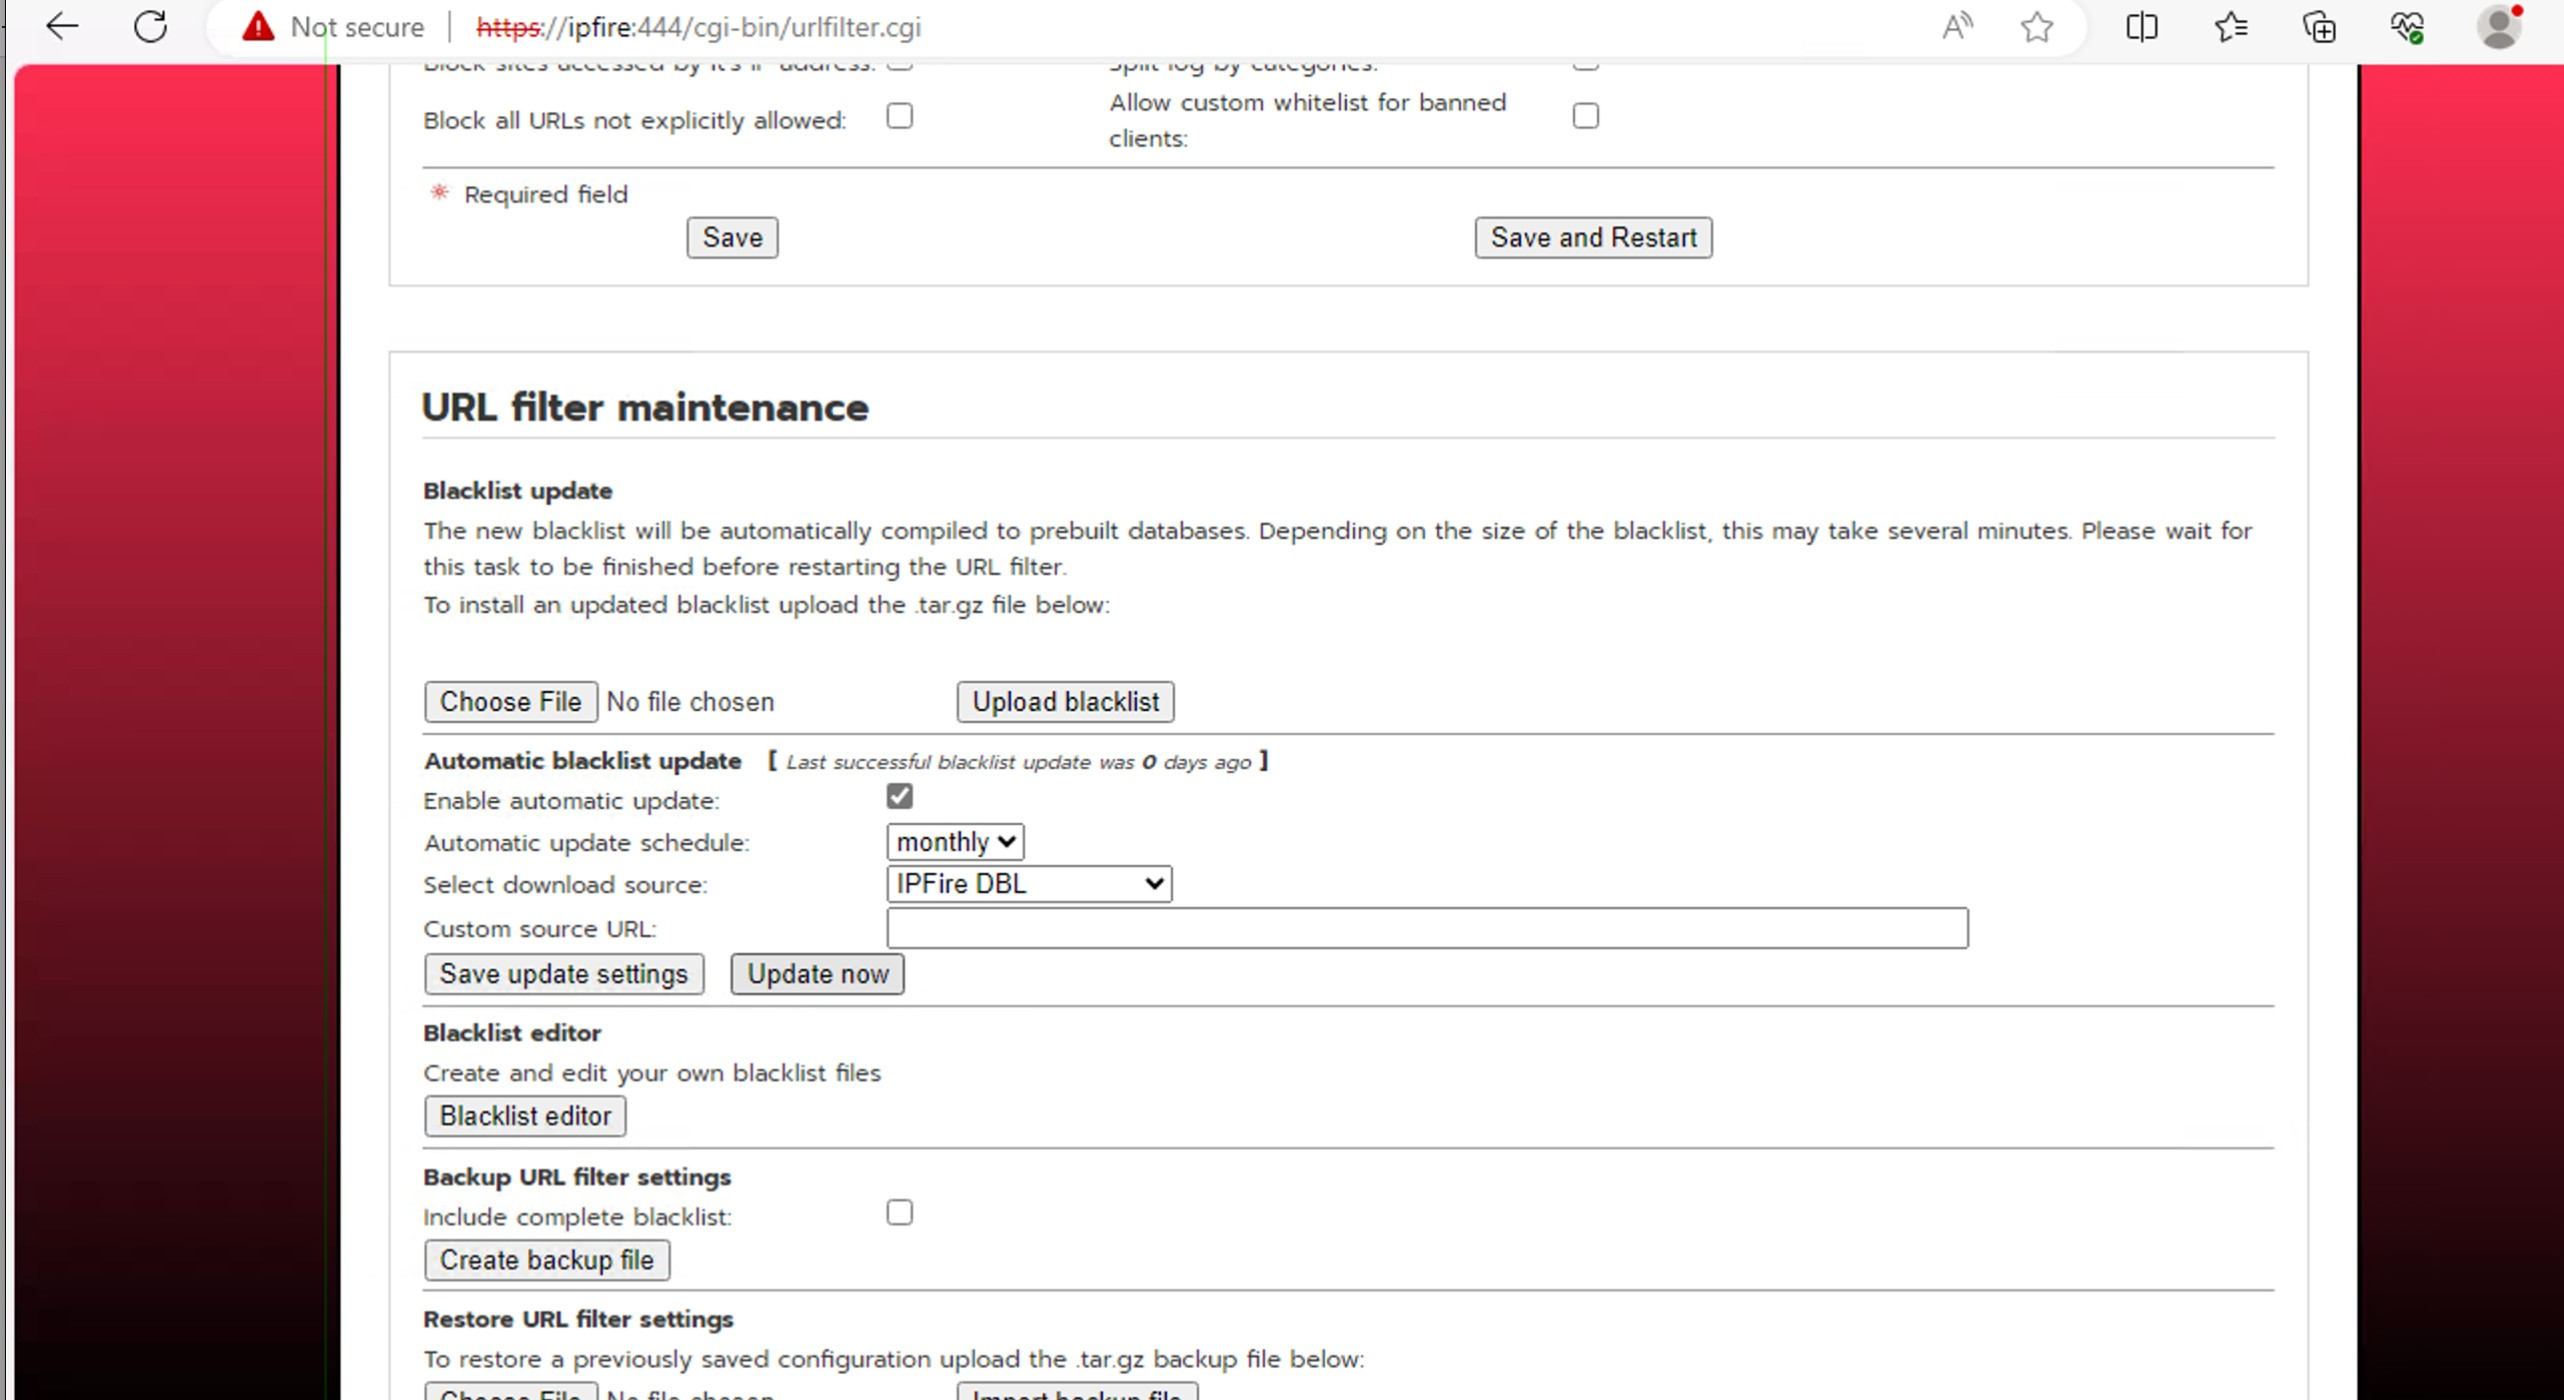
\includegraphics[width=0.9\textwidth]{media/ipfire/20.jpg}
	\caption{Aktualizacja listy IPFire DBL}
	\label{fig:ipf_20}
\end{figure}

Po aktualizacji listy można wybrać kategorie strone, które chcemy blokować. Można też zdefiniować własne wpisy w czarnej i białej liście. W celach przykładu sprawdzimy czy blokowana będzie strona wp.pl oraz wybrana strona z listy IPFire DBL [Rys. \ref{fig:ipf_21}]
\begin{figure}[!htbp]
	\centering
	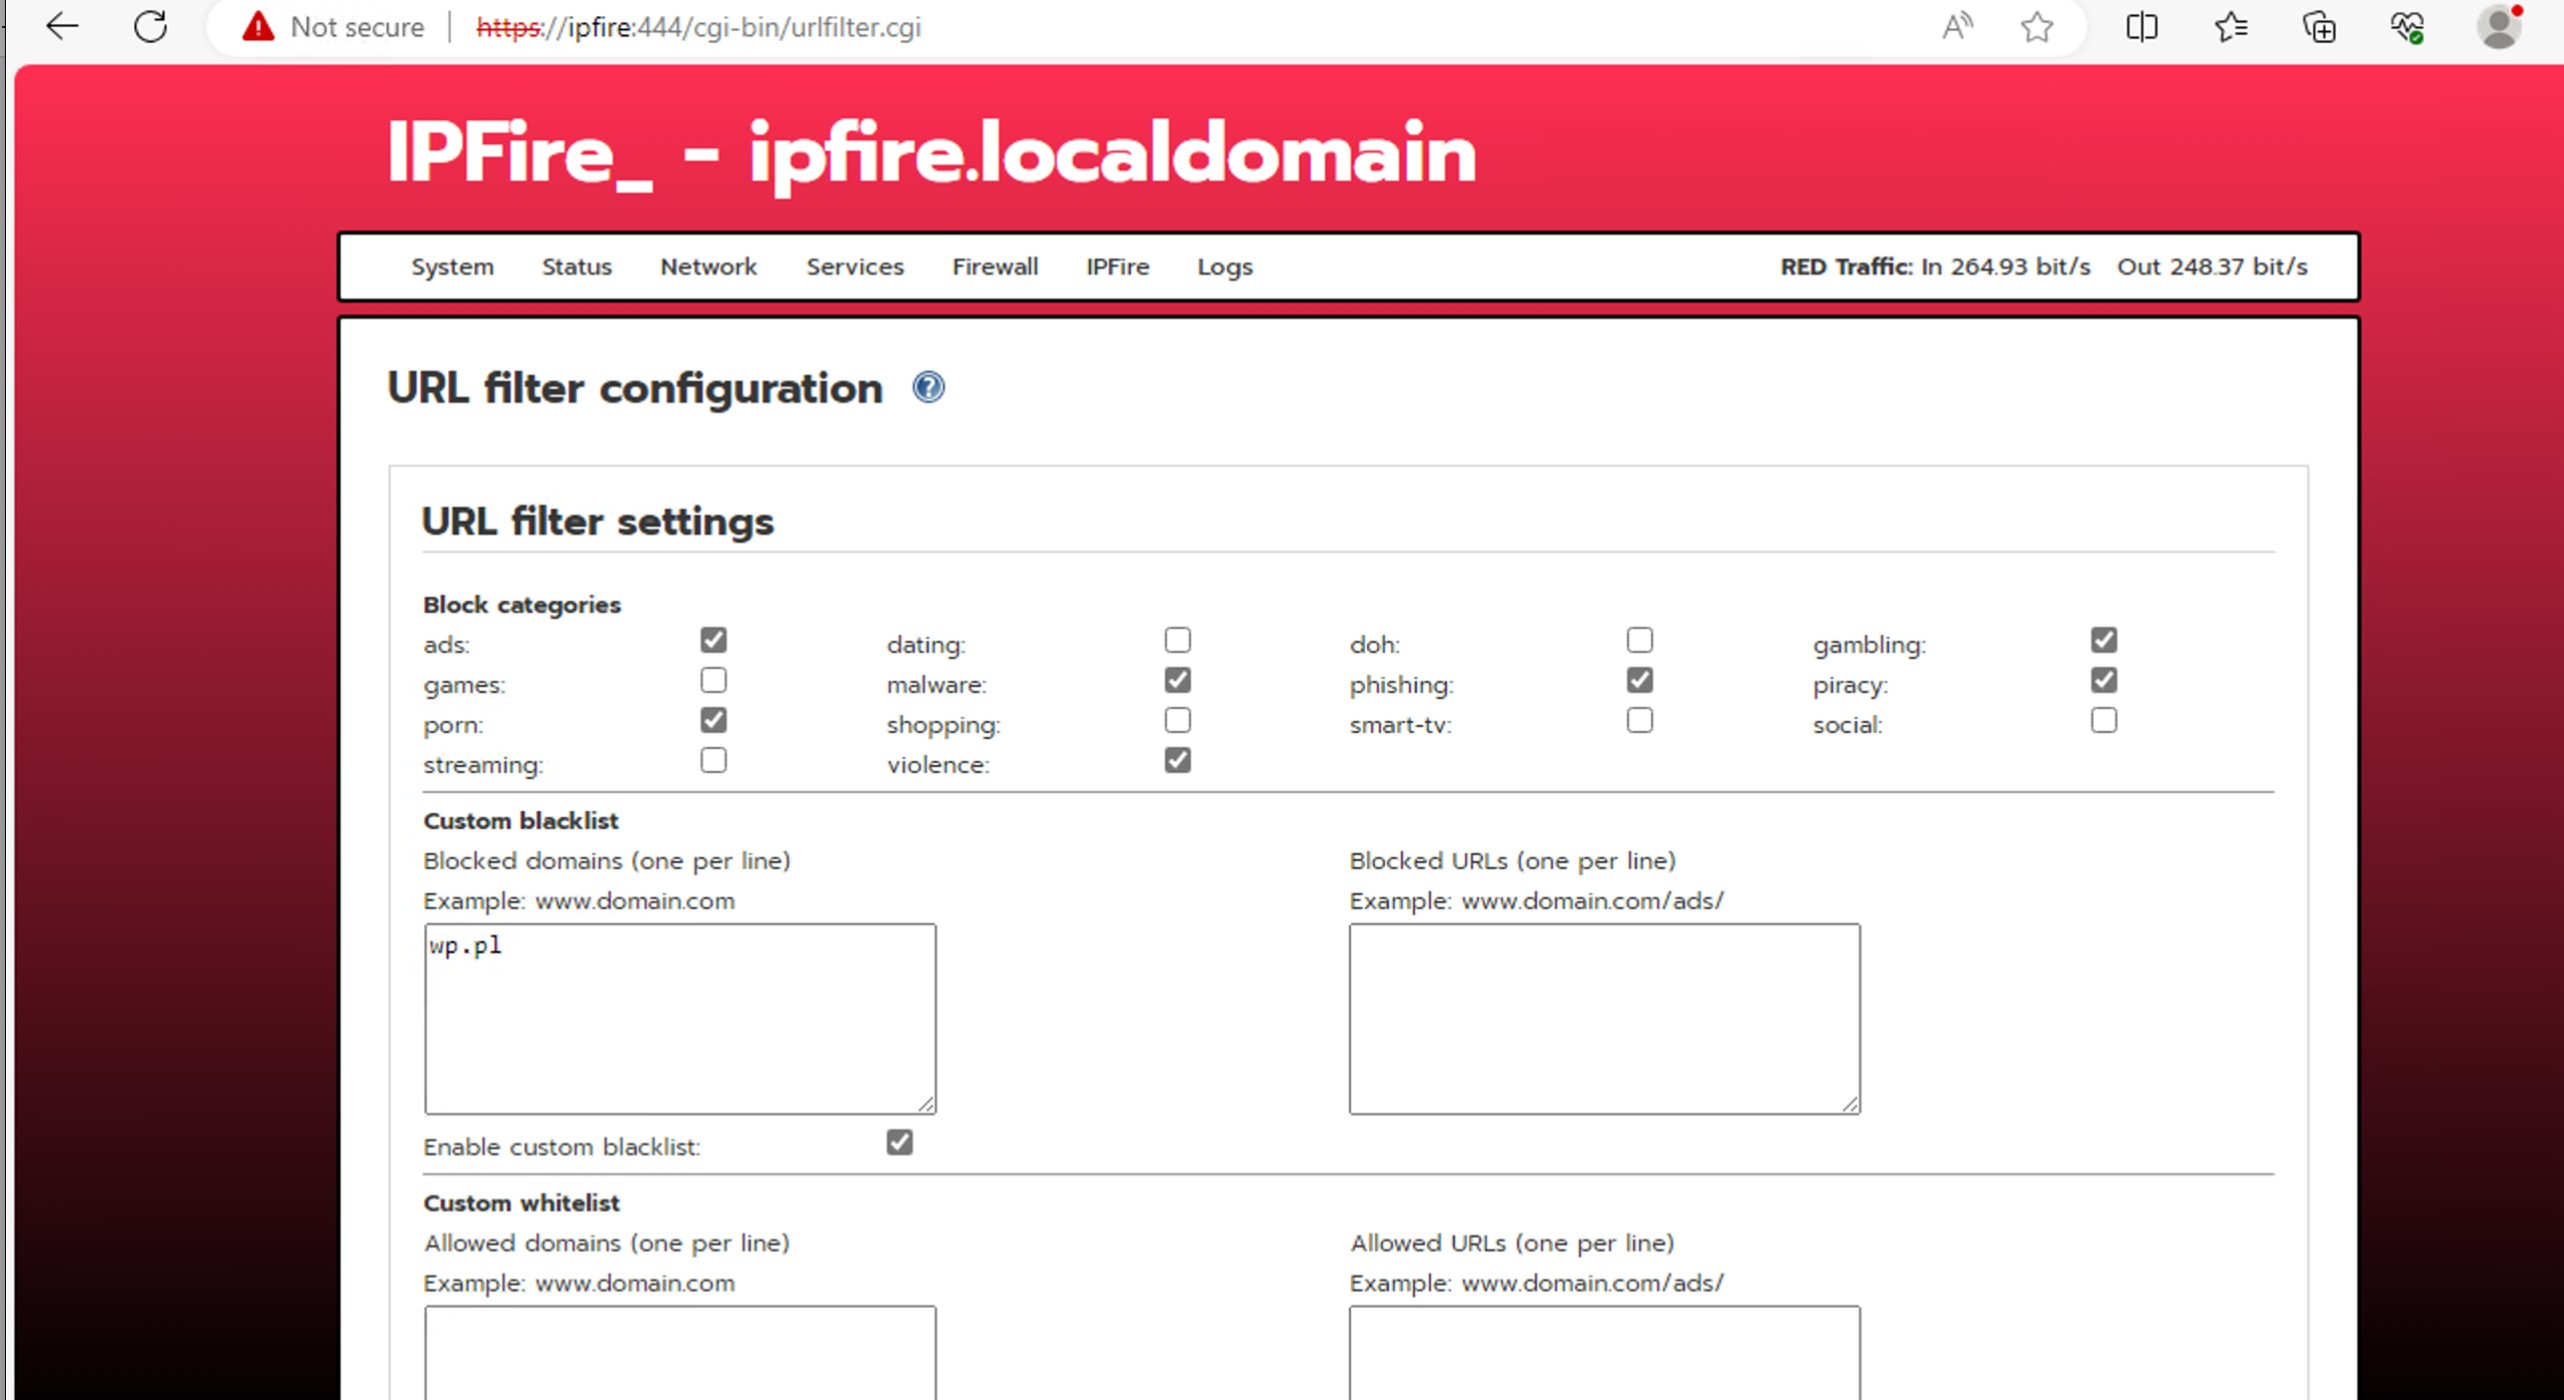
\includegraphics[width=0.9\textwidth]{media/ipfire/21.jpg}
	\caption{Definicja blokowanych treści}
	\label{fig:ipf_21}
\end{figure}

Strona wp.pl zgodnie z oczekiwaniami jest blokowana [Rys. \ref{fig:ipf_22}]
\begin{figure}[!htbp]
	\centering
	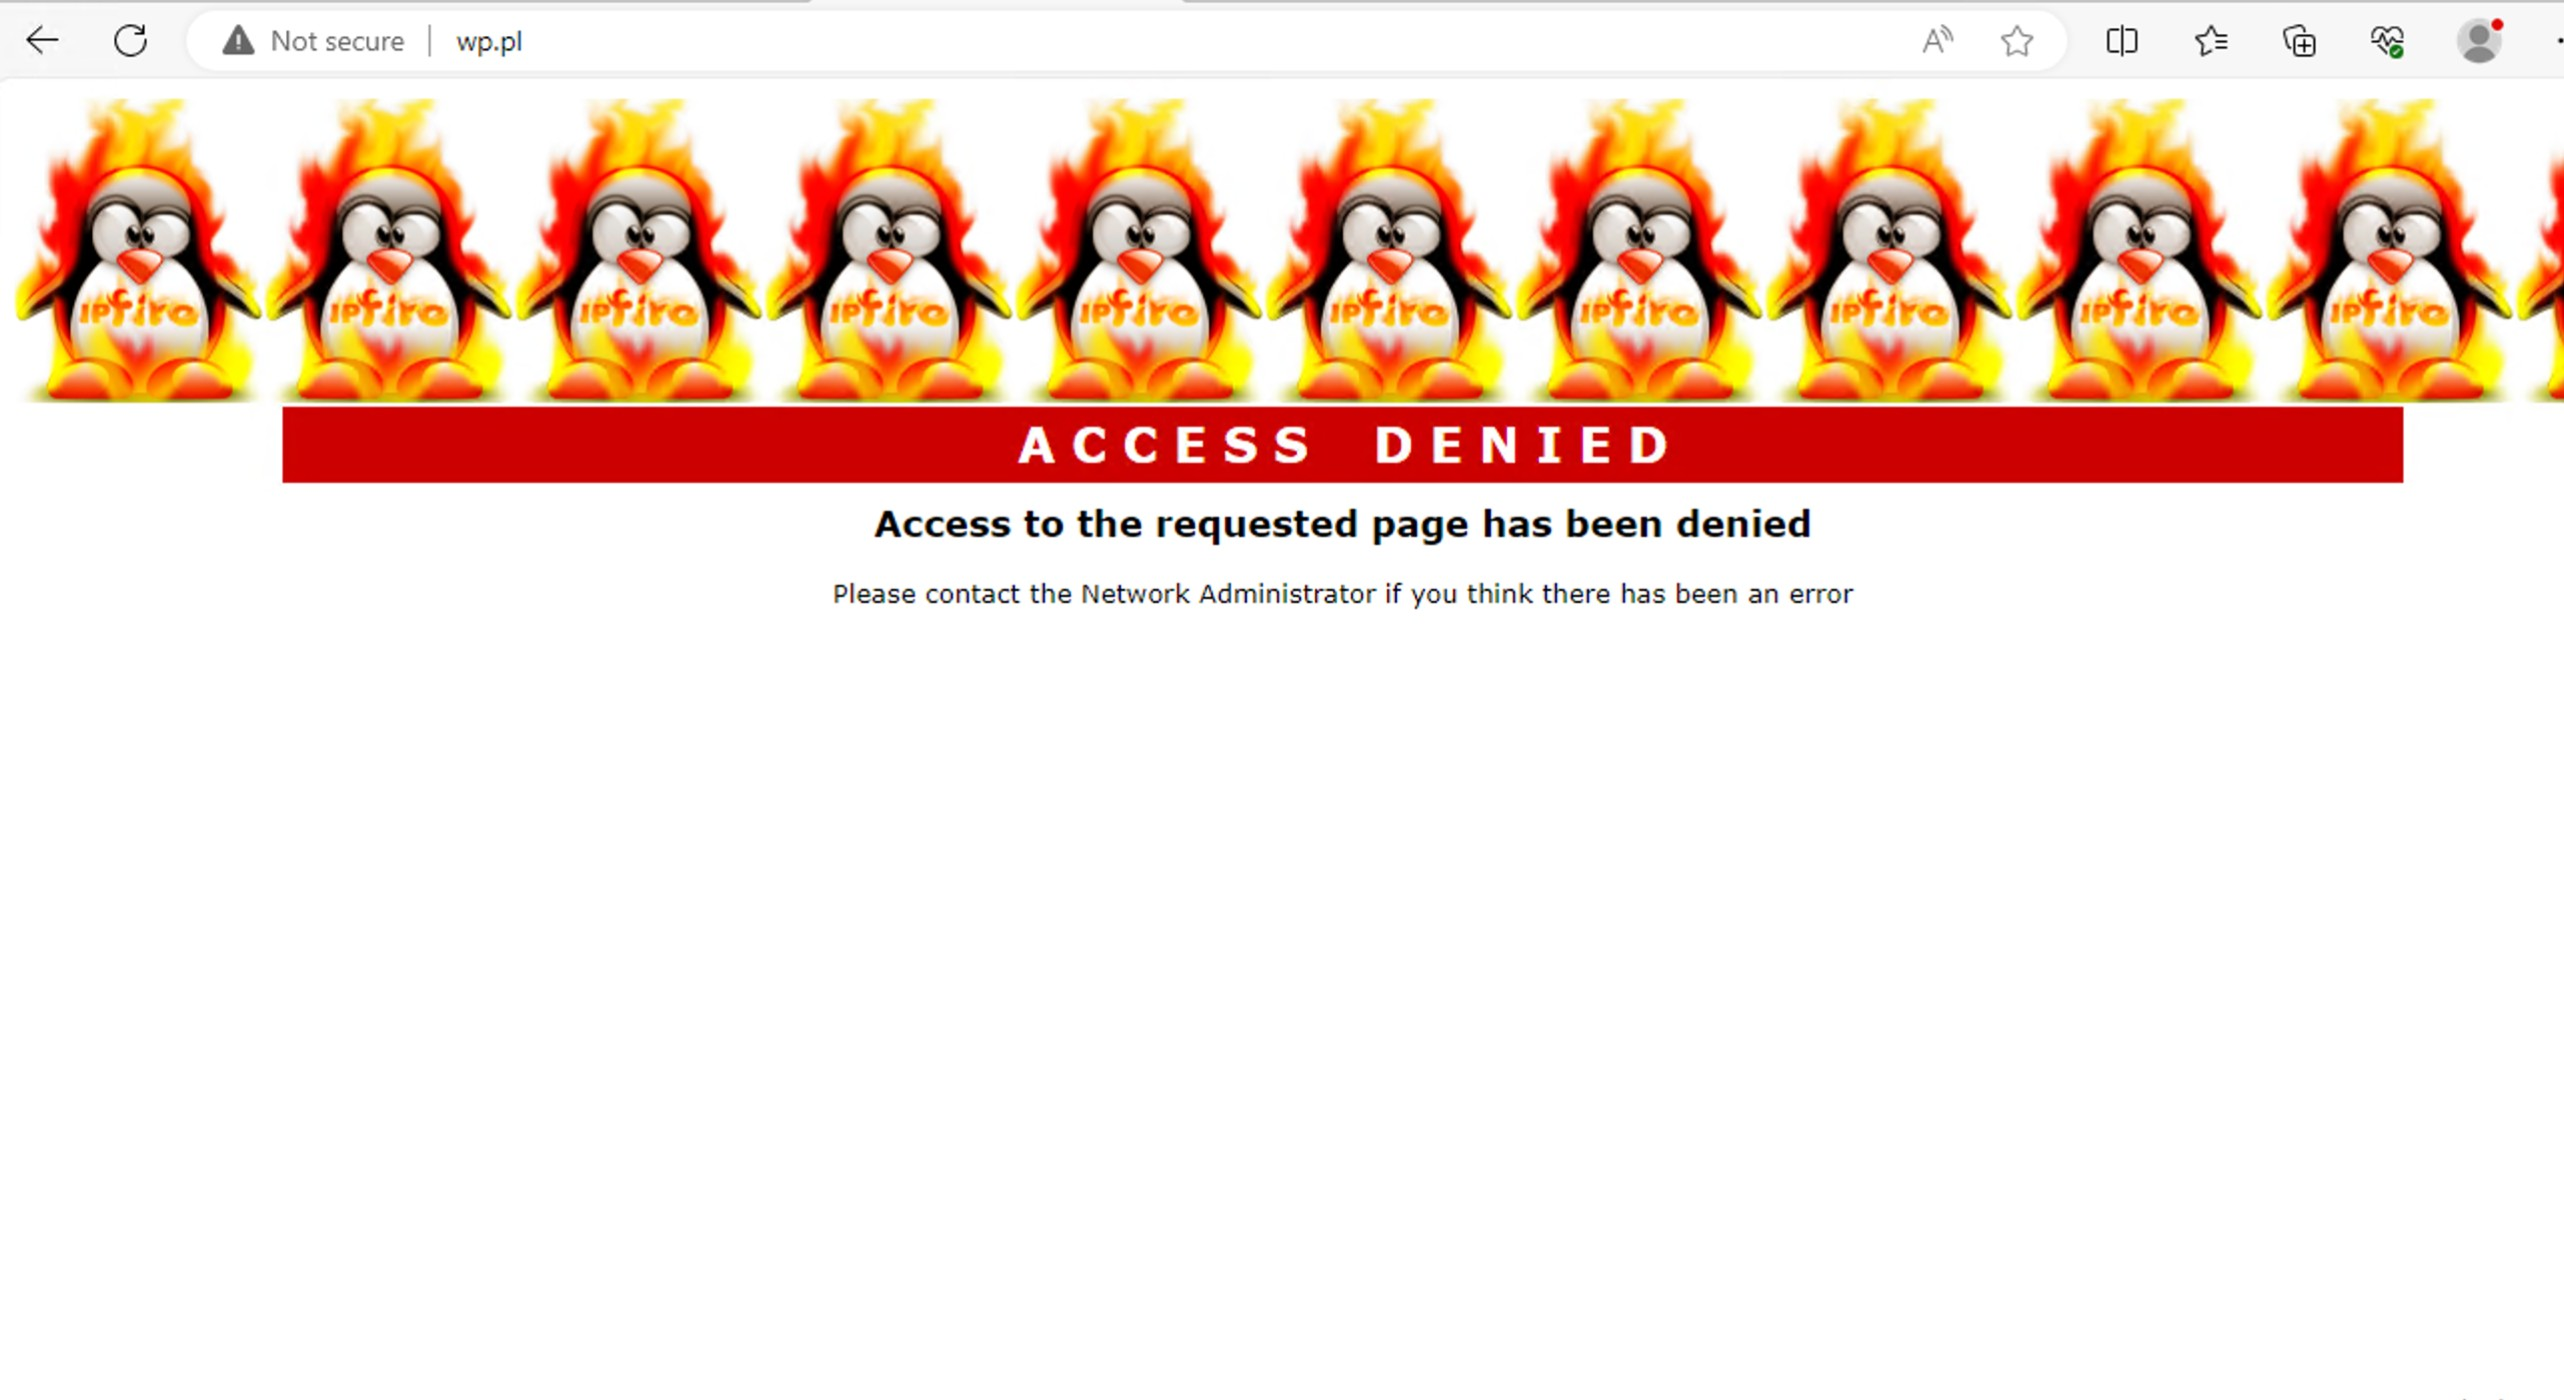
\includegraphics[width=0.9\textwidth]{media/ipfire/22.jpg}
	\caption{Blokowanie domeny zdefiniowanej ręcznie}
	\label{fig:ipf_22}
\end{figure}

Tak samo losowo wybrana strona z zaznaczonej w konfiguracji kategorii Malware z listy IPFire DBL [Rys. \ref{fig:ipf_23}]
\begin{figure}[!htbp]
	\centering
	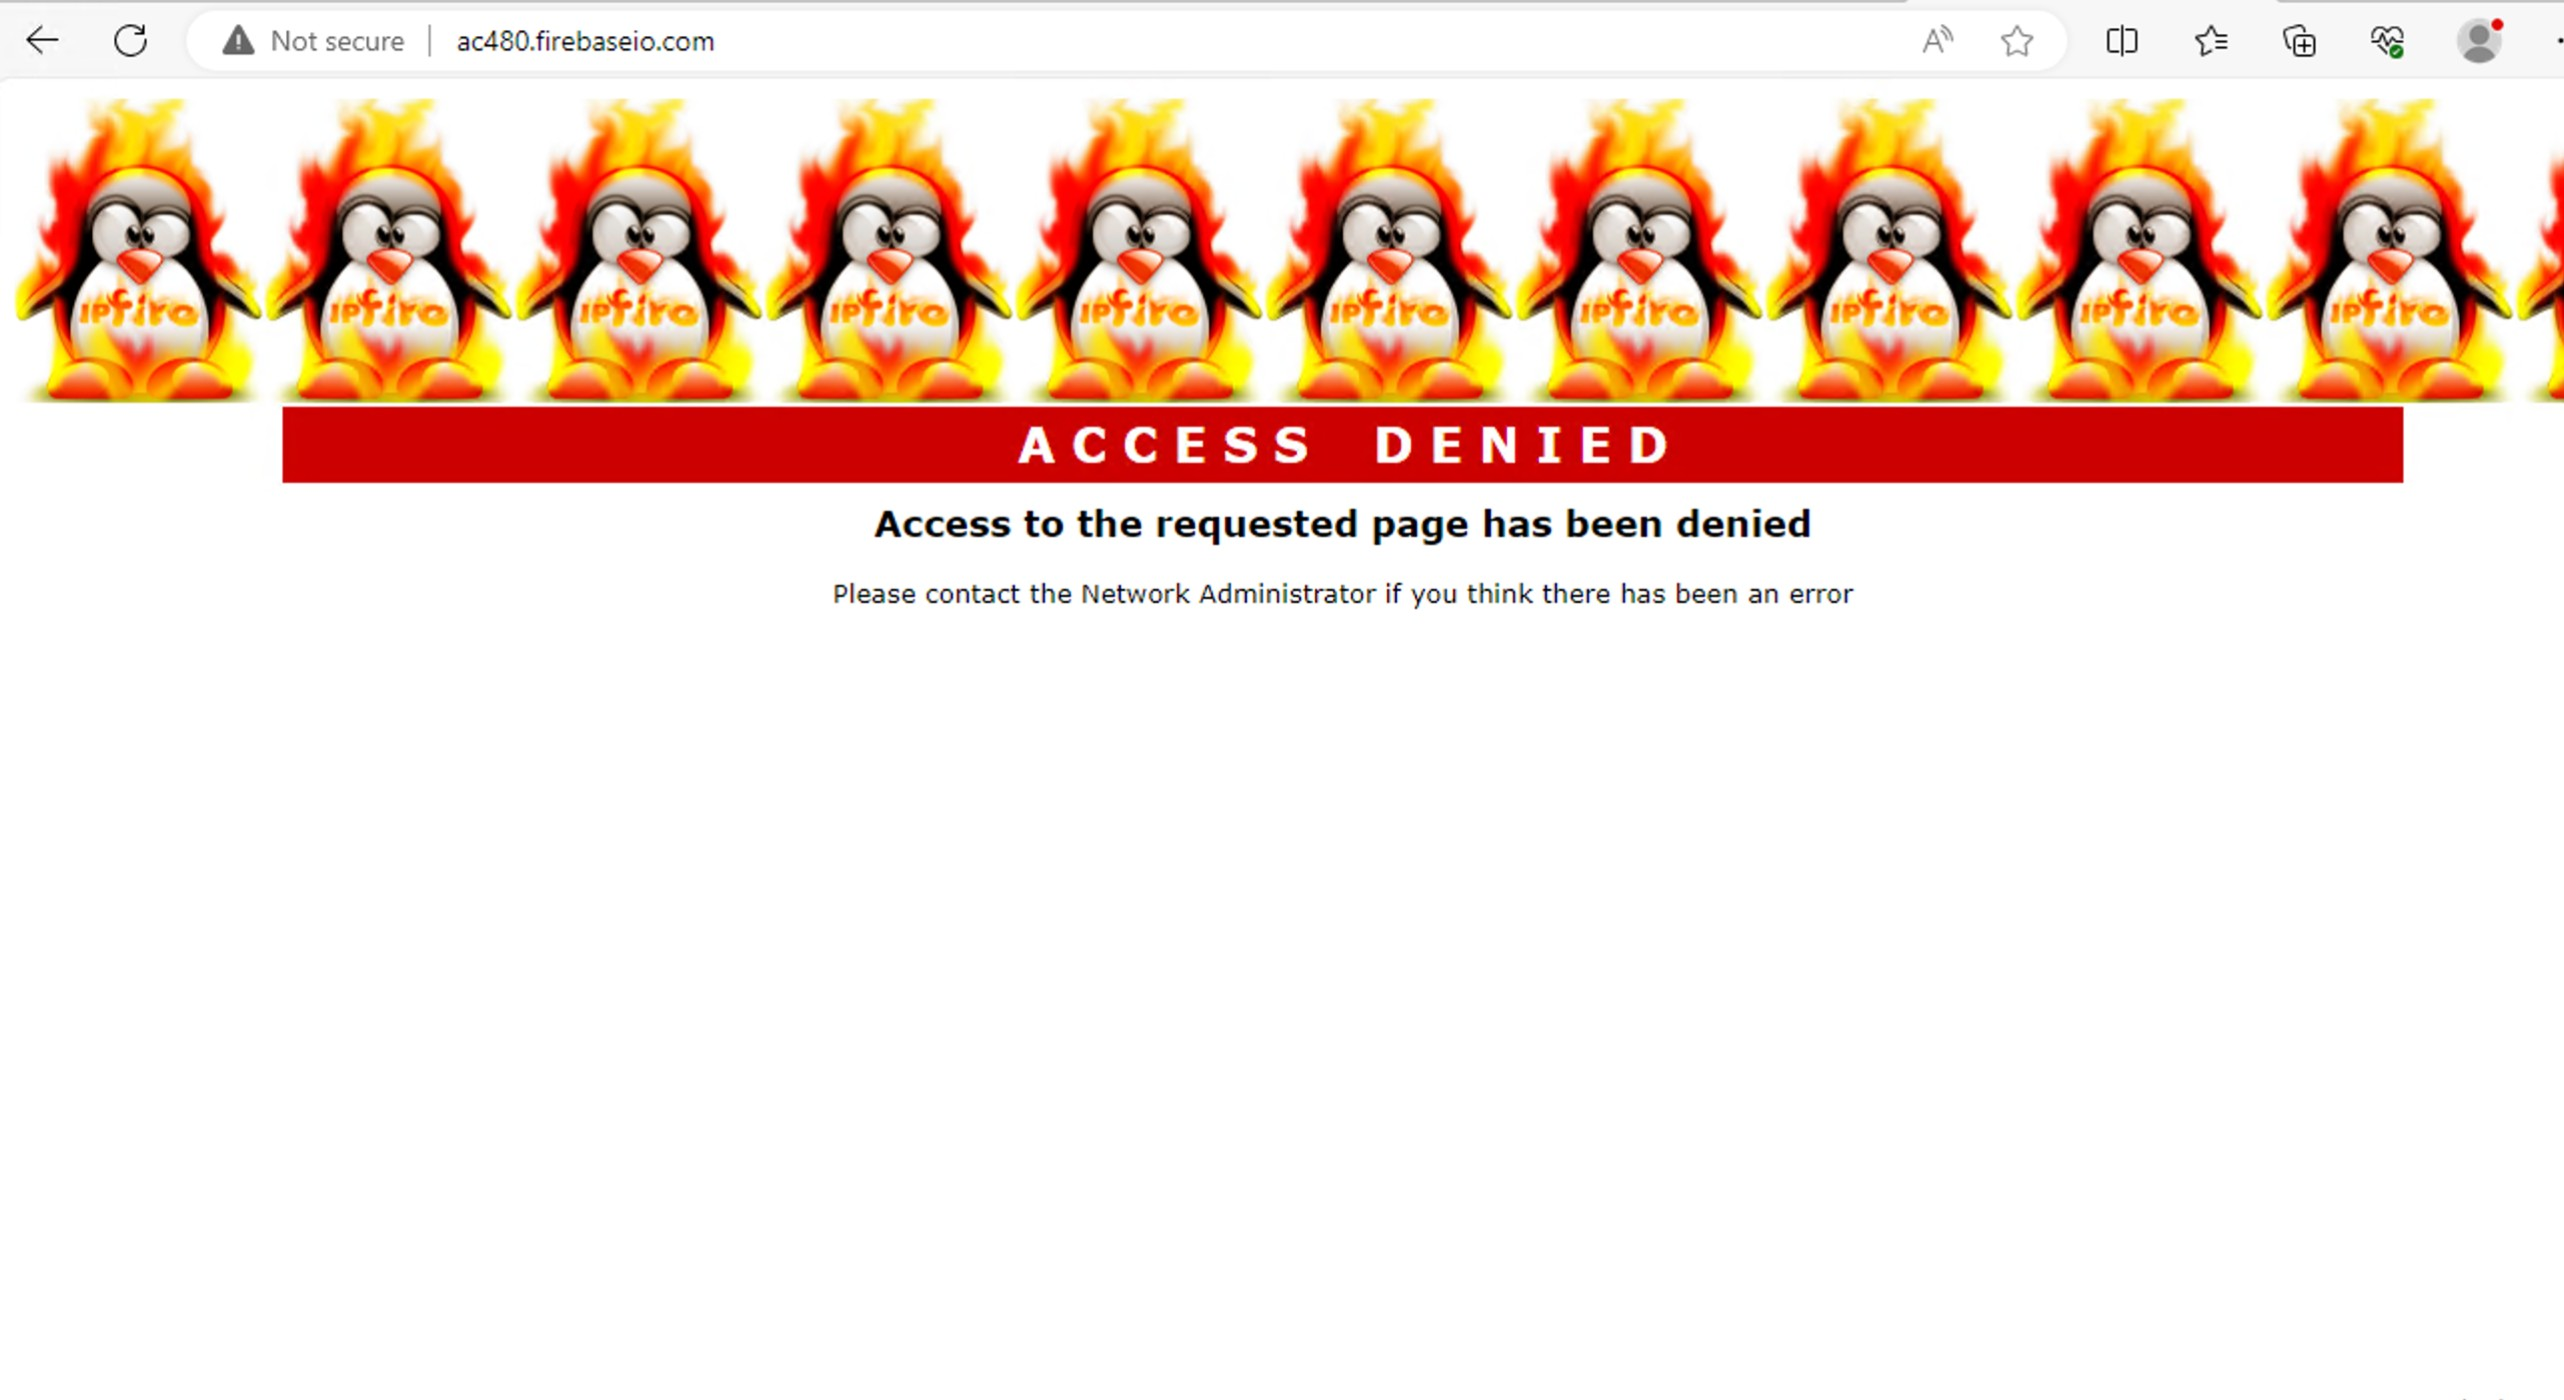
\includegraphics[width=0.9\textwidth]{media/ipfire/23.jpg}
	\caption{Blokowanie domeny z listy IPFire DBL}
	\label{fig:ipf_23}
\end{figure}

Pozostałe strony natomiast, jak np. YouTube, działają bez problemu, zgodnie z oczekiwaniami [Rys. \ref{fig:ipf_24}]
\begin{figure}[!htbp]
	\centering
	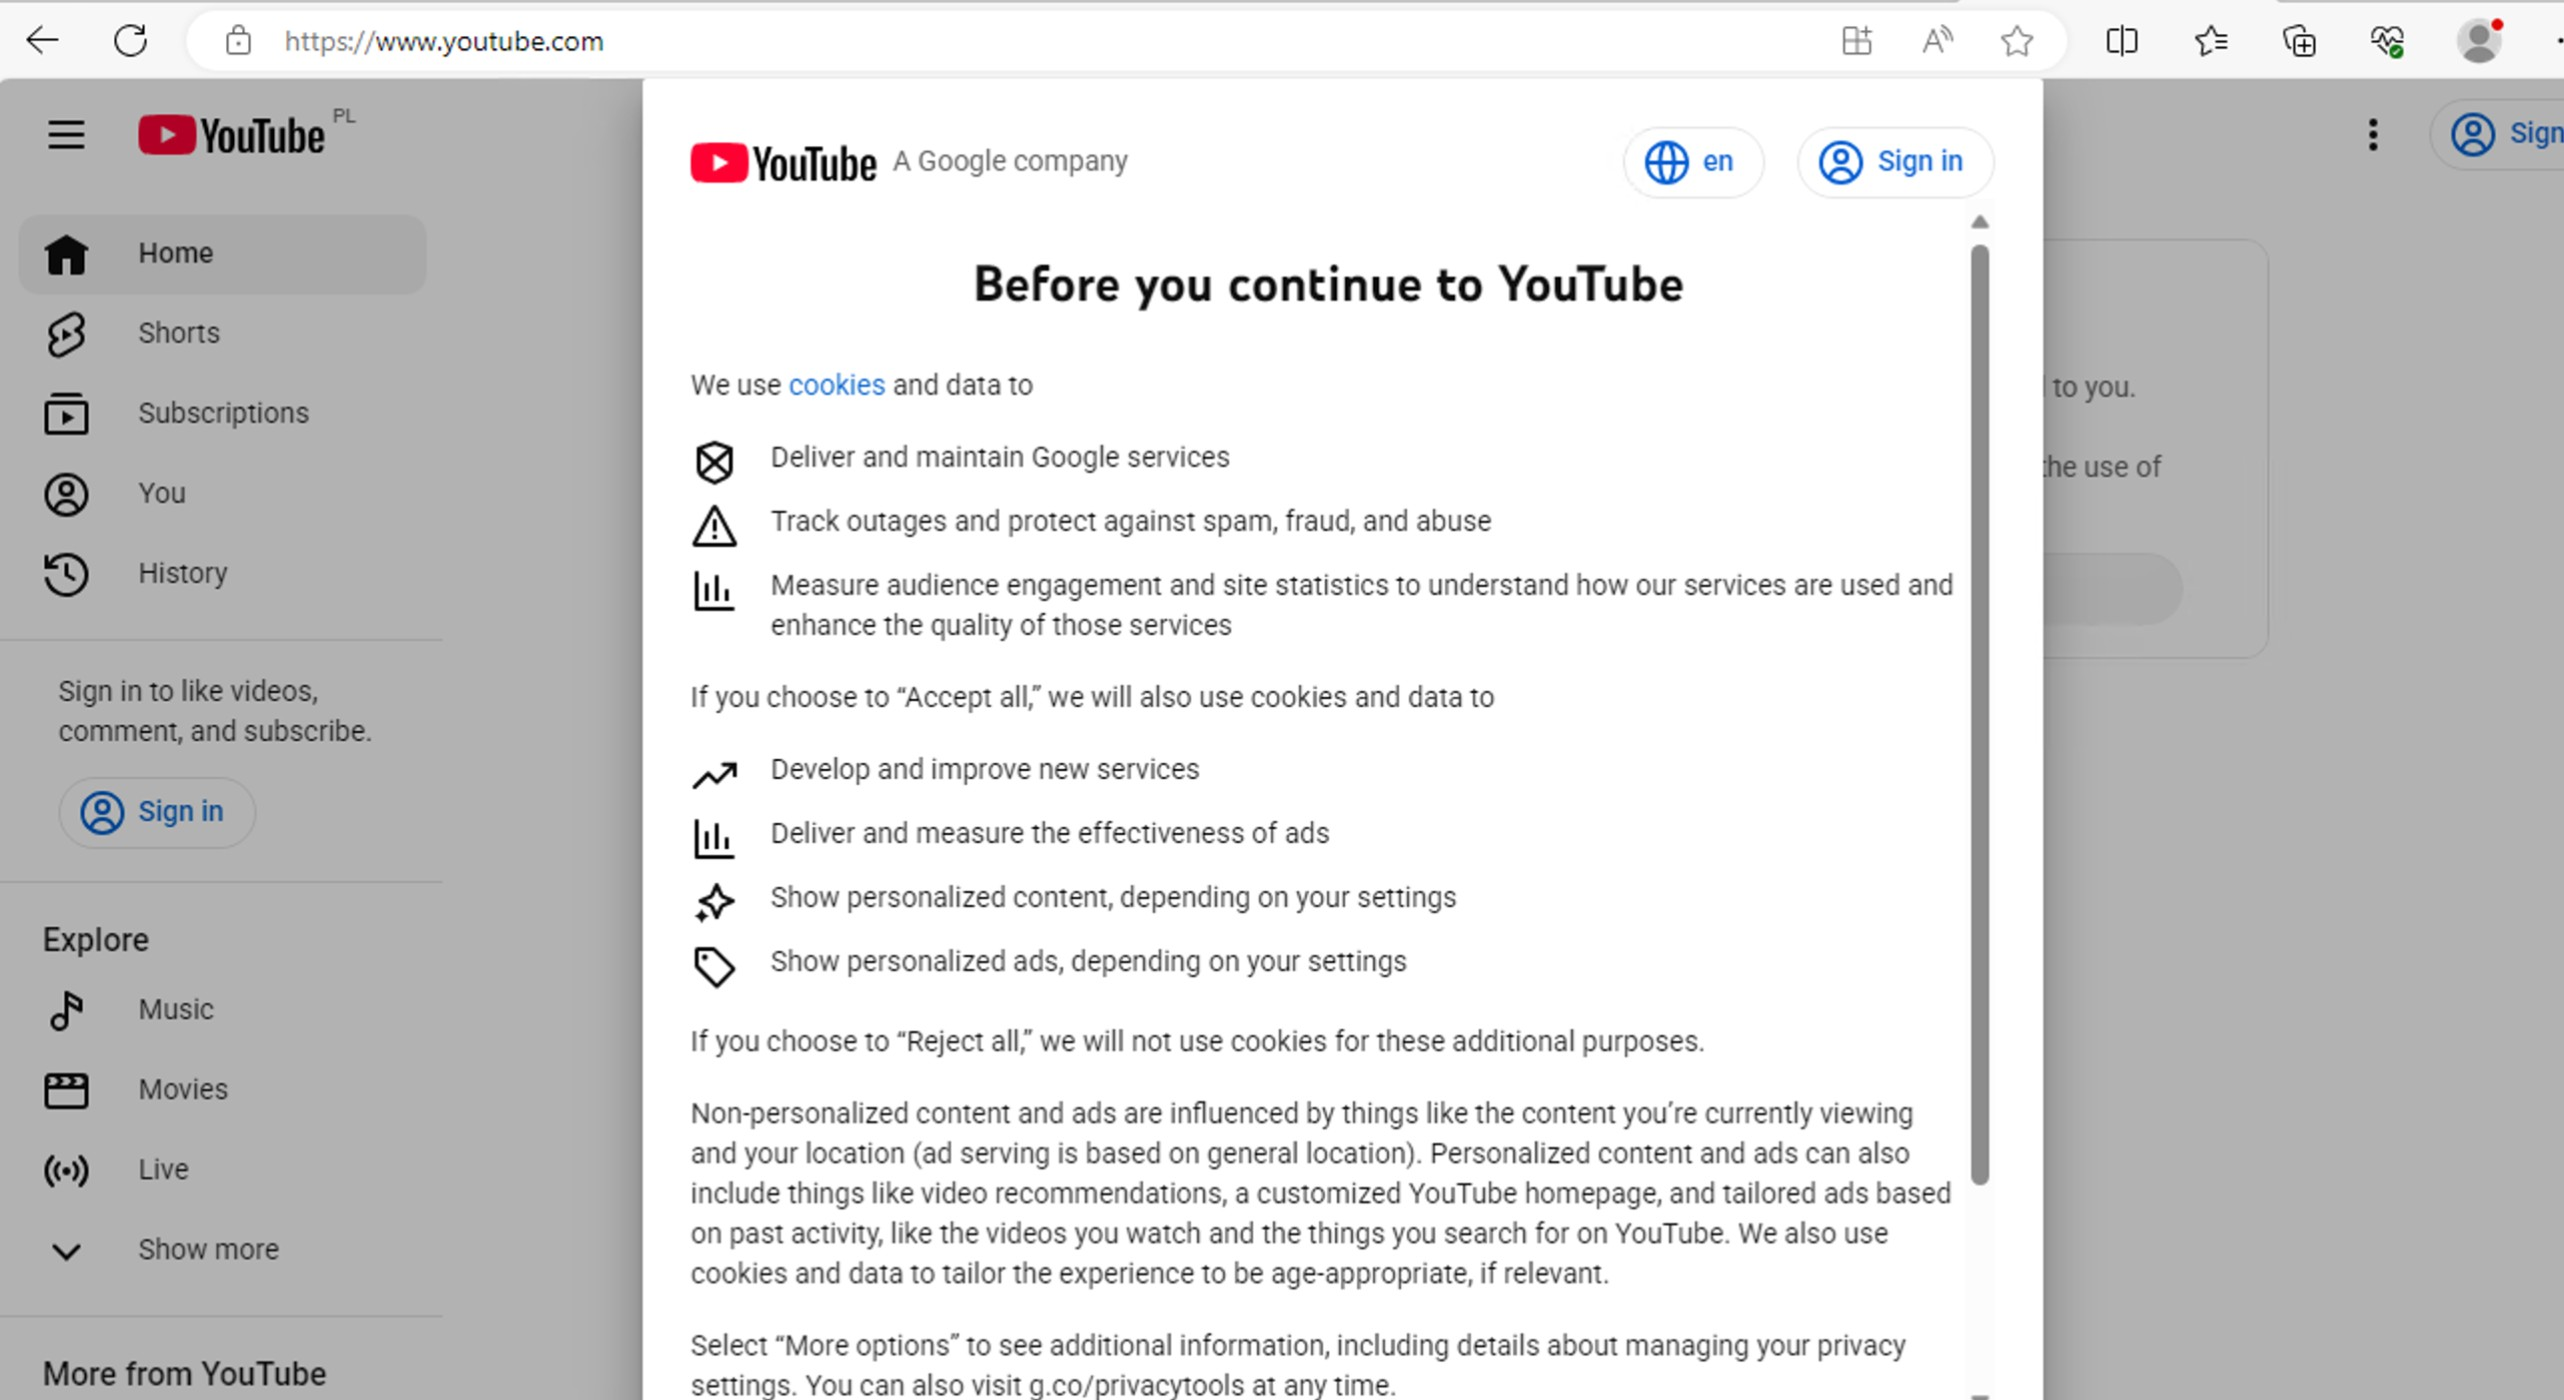
\includegraphics[width=0.9\textwidth]{media/ipfire/24.jpg}
	\caption{Bezpieczne treści nie są blokowane}
	\label{fig:ipf_24}
\end{figure}

\newpage











\section{Podsumowanie}
Podsumowując, wszystkie analizowane rozwiązania należą do grupy otwartoźródłowych systemów sieciowych, jednak różnią się podejściem do architektury, poziomem zaawansowania oraz docelowymi zastosowaniami.

pfSense i OPNsense stanowią najbardziej rozbudowane platformy firewall klasy enterprise wśród omawianych rozwiązań. Oba systemy bazują na FreeBSD i wykorzystują mechanizm filtrowania pakietów pf, oferując szeroki wachlarz funkcji, wysoką wydajność oraz zaawansowane możliwości konfiguracji. pfSense jest rozwiązaniem bardziej dojrzałym i szeroko rozpowszechnionym, jednak jego architektura pozostaje w dużej mierze monolityczna i mniej nowoczesna. OPNsense natomiast rozwija się w kierunku większej przejrzystości i bezpieczeństwa, oferując nowoczesną architekturę opartą na MVC, natywne API oraz bardziej uporządkowany cykl wydawniczy.

IPFire reprezentuje podejście pośrednie, jest systemem opartym na jądrze Linux, który kładzie silny nacisk na bezpieczeństwo, prostotę oraz stabilność. Dzięki modularnej architekturze i systemowi dodatków (Pakfire) oferuje elastyczność, jednak nie dorównuje pfSense i OPNsense pod względem liczby funkcji, nowoczesności czy rozbudowania ekosystemu. Jego zaletą jest natomiast łatwość konfiguracji oraz dobre wsparcie dla różnych platform sprzętowych, w tym architektury ARM.

OpenWRT wyróżnia się na tle pozostałych rozwiązań największą elastycznością i wsparciem sprzętowym, szczególnie w kontekście urządzeń embedded i routerów konsumenckich. Jest to w pełni modularna dystrybucja Linuxa, która może pełnić funkcję zarówno prostego routera, jak i zaawansowanej platformy sieciowej. O ile pełnienie funkcji zaawansowanej zapory sieciowej nie jest jego głównym założeniem, instalacja tego oprogramowania na sprzęcie niewspieranym już przez producenta może znacząco podnieść poziom bezpieczeństwa sieci. Jednocześnie wymaga ono większej wiedzy technicznej od użytkownika i nie oferuje tak rozbudowanych, gotowych mechanizmów bezpieczeństwa „out of the box” jak pozostałe systemy.

W rezultacie wybór odpowiedniego rozwiązania zależy od konkretnego zastosowania: pfSense i OPNsense najlepiej sprawdzają się w środowiskach wymagających zaawansowanej kontroli i funkcjonalności, IPFire stanowi kompromis pomiędzy bezpieczeństwem a prostotą, natomiast OpenWRT jest najbardziej elastycznym rozwiązaniem dla użytkowników potrzebujących pełnej kontroli nad systemem, szczególnie na niestandardowym sprzęcie.



\newpage
\section{Wnioski}
\begin{itemize}
    \item \textbf{Spostrzeżenia:} Rozwiązania otwartoźródłowe takie jak OPNsense, pfSense, IPFire oraz OpenWrt oferują zaawansowane możliwości, które nierzadko dorównują lub wręcz przewyższają funkcjonalności komercyjnych systemów firewall. Różnice w architekturze (FreeBSD vs Linux) oraz w podejściu do zarządzania sprawiają, że każdy z systemów znajduje swoje unikalne zastosowanie --- od domowych routerów po rozbudowane sieci korporacyjne.
    \item \textbf{Osiągnięcia:} W ramach projektu pomyślnie przeprowadzono analizę porównawczą wybranych systemów, identyfikując ich mocne i słabe strony. Ponadto, z powodzeniem wdrożono i skonfigurowano środowisko testowe oparte na systemie IPFire. Udowodniono w praktyce łatwość implementacji podstawowych polityk bezpieczeństwa, takich jak filtrowanie treści przy użyciu wbudowanego proxy i mechanizmu URL Filter.
    \item \textbf{Potencjał rozwoju:} Opracowane środowisko testowe może stanowić punkt wyjścia do dalszych badań. Naturalnym rozwinięciem projektu byłoby wdrożenie i porównanie wydajności badanych systemów (np. IPFire vs OPNsense) w warunkach dużego obciążenia sieciowego, a także przetestowanie bardziej zaawansowanych mechanizmów, takich jak systemy detekcji i prewencji włamań (IDS/IPS - np. Suricata, Zeek) czy zaawansowane tunele VPN (WireGuard, IPsec) działające w topologii site-to-site.
\end{itemize}





\newpage
\section{Bibliografia}
\begin{enumerate}
	\item Historia forka OPNsense: https://docs.opnsense.org/history/thefork.html
	\item pfSense 2023 XSS vulnerability: https://thehackernews.com/2023/12/new-security-vulnerabilities-uncovered.html
	\item Funkcje OPNsense: https://opnsense.org/wp-content/uploads/2025/11/OPNsense-Whitepaper-features-NIEUW.pdf
	\item Wymagania sprzętowe OPNsense: https://docs.opnsense.org/manual/hardware.html
	\item Minimalne wymagania sprzętowe pfSense: https://docs.netgate.com/pfsense/en/latest/hardware/minimum-requirements.html
	\item Ogólne informacje o projekcie IPFire: https://de.wikipedia.org/wiki/IPFire
	\item Informacje techniczne na temat projektu IPFire: https://www.ipfire.org/docs
	\item Oficjalna dokumentacja OpenWrt: https://openwrt.org/docs/start
	\item Historia projektu OpenWrt: https://openwrt.org/about/history
\end{enumerate}

\end{document}